\documentclass[]{article}
\usepackage{lmodern}
\usepackage{amssymb,amsmath}
\usepackage{ifxetex,ifluatex}
\usepackage{fixltx2e} % provides \textsubscript
\ifnum 0\ifxetex 1\fi\ifluatex 1\fi=0 % if pdftex
  \usepackage[T1]{fontenc}
  \usepackage[utf8]{inputenc}
\else % if luatex or xelatex
  \ifxetex
    \usepackage{mathspec}
  \else
    \usepackage{fontspec}
  \fi
  \defaultfontfeatures{Ligatures=TeX,Scale=MatchLowercase}
\fi
% use upquote if available, for straight quotes in verbatim environments
\IfFileExists{upquote.sty}{\usepackage{upquote}}{}
% use microtype if available
\IfFileExists{microtype.sty}{%
\usepackage{microtype}
\UseMicrotypeSet[protrusion]{basicmath} % disable protrusion for tt fonts
}{}
\usepackage[margin=1in]{geometry}
\usepackage{hyperref}
\hypersetup{unicode=true,
            pdftitle={Lobbying the U.S. Federal Energy Regulatory Commission (FERC)},
            pdfborder={0 0 0},
            breaklinks=true}
\urlstyle{same}  % don't use monospace font for urls
\usepackage{color}
\usepackage{fancyvrb}
\newcommand{\VerbBar}{|}
\newcommand{\VERB}{\Verb[commandchars=\\\{\}]}
\DefineVerbatimEnvironment{Highlighting}{Verbatim}{commandchars=\\\{\}}
% Add ',fontsize=\small' for more characters per line
\usepackage{framed}
\definecolor{shadecolor}{RGB}{248,248,248}
\newenvironment{Shaded}{\begin{snugshade}}{\end{snugshade}}
\newcommand{\KeywordTok}[1]{\textcolor[rgb]{0.13,0.29,0.53}{\textbf{#1}}}
\newcommand{\DataTypeTok}[1]{\textcolor[rgb]{0.13,0.29,0.53}{#1}}
\newcommand{\DecValTok}[1]{\textcolor[rgb]{0.00,0.00,0.81}{#1}}
\newcommand{\BaseNTok}[1]{\textcolor[rgb]{0.00,0.00,0.81}{#1}}
\newcommand{\FloatTok}[1]{\textcolor[rgb]{0.00,0.00,0.81}{#1}}
\newcommand{\ConstantTok}[1]{\textcolor[rgb]{0.00,0.00,0.00}{#1}}
\newcommand{\CharTok}[1]{\textcolor[rgb]{0.31,0.60,0.02}{#1}}
\newcommand{\SpecialCharTok}[1]{\textcolor[rgb]{0.00,0.00,0.00}{#1}}
\newcommand{\StringTok}[1]{\textcolor[rgb]{0.31,0.60,0.02}{#1}}
\newcommand{\VerbatimStringTok}[1]{\textcolor[rgb]{0.31,0.60,0.02}{#1}}
\newcommand{\SpecialStringTok}[1]{\textcolor[rgb]{0.31,0.60,0.02}{#1}}
\newcommand{\ImportTok}[1]{#1}
\newcommand{\CommentTok}[1]{\textcolor[rgb]{0.56,0.35,0.01}{\textit{#1}}}
\newcommand{\DocumentationTok}[1]{\textcolor[rgb]{0.56,0.35,0.01}{\textbf{\textit{#1}}}}
\newcommand{\AnnotationTok}[1]{\textcolor[rgb]{0.56,0.35,0.01}{\textbf{\textit{#1}}}}
\newcommand{\CommentVarTok}[1]{\textcolor[rgb]{0.56,0.35,0.01}{\textbf{\textit{#1}}}}
\newcommand{\OtherTok}[1]{\textcolor[rgb]{0.56,0.35,0.01}{#1}}
\newcommand{\FunctionTok}[1]{\textcolor[rgb]{0.00,0.00,0.00}{#1}}
\newcommand{\VariableTok}[1]{\textcolor[rgb]{0.00,0.00,0.00}{#1}}
\newcommand{\ControlFlowTok}[1]{\textcolor[rgb]{0.13,0.29,0.53}{\textbf{#1}}}
\newcommand{\OperatorTok}[1]{\textcolor[rgb]{0.81,0.36,0.00}{\textbf{#1}}}
\newcommand{\BuiltInTok}[1]{#1}
\newcommand{\ExtensionTok}[1]{#1}
\newcommand{\PreprocessorTok}[1]{\textcolor[rgb]{0.56,0.35,0.01}{\textit{#1}}}
\newcommand{\AttributeTok}[1]{\textcolor[rgb]{0.77,0.63,0.00}{#1}}
\newcommand{\RegionMarkerTok}[1]{#1}
\newcommand{\InformationTok}[1]{\textcolor[rgb]{0.56,0.35,0.01}{\textbf{\textit{#1}}}}
\newcommand{\WarningTok}[1]{\textcolor[rgb]{0.56,0.35,0.01}{\textbf{\textit{#1}}}}
\newcommand{\AlertTok}[1]{\textcolor[rgb]{0.94,0.16,0.16}{#1}}
\newcommand{\ErrorTok}[1]{\textcolor[rgb]{0.64,0.00,0.00}{\textbf{#1}}}
\newcommand{\NormalTok}[1]{#1}
\usepackage{longtable,booktabs}
\usepackage{graphicx,grffile}
\makeatletter
\def\maxwidth{\ifdim\Gin@nat@width>\linewidth\linewidth\else\Gin@nat@width\fi}
\def\maxheight{\ifdim\Gin@nat@height>\textheight\textheight\else\Gin@nat@height\fi}
\makeatother
% Scale images if necessary, so that they will not overflow the page
% margins by default, and it is still possible to overwrite the defaults
% using explicit options in \includegraphics[width, height, ...]{}
\setkeys{Gin}{width=\maxwidth,height=\maxheight,keepaspectratio}
\IfFileExists{parskip.sty}{%
\usepackage{parskip}
}{% else
\setlength{\parindent}{0pt}
\setlength{\parskip}{6pt plus 2pt minus 1pt}
}
\setlength{\emergencystretch}{3em}  % prevent overfull lines
\providecommand{\tightlist}{%
  \setlength{\itemsep}{0pt}\setlength{\parskip}{0pt}}
\setcounter{secnumdepth}{0}
% Redefines (sub)paragraphs to behave more like sections
\ifx\paragraph\undefined\else
\let\oldparagraph\paragraph
\renewcommand{\paragraph}[1]{\oldparagraph{#1}\mbox{}}
\fi
\ifx\subparagraph\undefined\else
\let\oldsubparagraph\subparagraph
\renewcommand{\subparagraph}[1]{\oldsubparagraph{#1}\mbox{}}
\fi

%%% Use protect on footnotes to avoid problems with footnotes in titles
\let\rmarkdownfootnote\footnote%
\def\footnote{\protect\rmarkdownfootnote}

%%% Change title format to be more compact
\usepackage{titling}

% Create subtitle command for use in maketitle
\newcommand{\subtitle}[1]{
  \posttitle{
    \begin{center}\large#1\end{center}
    }
}

\setlength{\droptitle}{-2em}

  \title{Lobbying the U.S. Federal Energy Regulatory Commission (FERC)}
    \pretitle{\vspace{\droptitle}\centering\huge}
  \posttitle{\par}
    \author{}
    \preauthor{}\postauthor{}
    \date{}
    \predate{}\postdate{}
  

\begin{document}
\maketitle

\section{Data}\label{data}

\begin{Shaded}
\begin{Highlighting}[]
\KeywordTok{load}\NormalTok{(}\KeywordTok{here}\NormalTok{(}\StringTok{"data/all_contacts.RData"}\NormalTok{))}
\CommentTok{# one obs per member per letter for all agencies}
\NormalTok{d <-}\StringTok{ }\NormalTok{all_contacts }\OperatorTok{%>%}\StringTok{ }
\StringTok{  }\KeywordTok{ungroup}\NormalTok{() }\OperatorTok{%>%}\StringTok{ }
\StringTok{  }\CommentTok{# define d as just FERC}
\StringTok{  }\KeywordTok{filter}\NormalTok{(agency}\OperatorTok{==}\StringTok{"DOE_FERC"}\NormalTok{) }\OperatorTok{%>%}\StringTok{ }
\StringTok{  }\KeywordTok{select}\NormalTok{(}\OperatorTok{-}\NormalTok{SUBJECT) }\OperatorTok{%>%}\StringTok{ }
\StringTok{  }\KeywordTok{mutate}\NormalTok{(}\DataTypeTok{majority =} \KeywordTok{ifelse}\NormalTok{(majority }\OperatorTok{==}\StringTok{ }\DecValTok{1}\NormalTok{, }\StringTok{"Majority"}\NormalTok{, }\StringTok{"Minority"}\NormalTok{)) }\OperatorTok{%>%}
\StringTok{  }\CommentTok{# }\AlertTok{FIXME}\CommentTok{ }
\StringTok{  }\CommentTok{# GOODE needs to be fixed in party switchers portion of merge.R}
\StringTok{  }\KeywordTok{filter}\NormalTok{(}\OperatorTok{!}\NormalTok{(last_name }\OperatorTok{==}\StringTok{ "GOODE"}\OperatorTok{&}\NormalTok{party }\OperatorTok{==}\StringTok{ "(I)"}\NormalTok{))}
  

\CommentTok{# one obs per member per letter per committee for all agencies}
\KeywordTok{load}\NormalTok{(}\KeywordTok{here}\NormalTok{(}\StringTok{"data/all_contacts_committees.RData"}\NormalTok{))}
\CommentTok{# define dcommittees as just FERC}
\NormalTok{dcommittees <-}\StringTok{ }\NormalTok{all_contacts_committees }\OperatorTok{%<>%}\StringTok{ }\KeywordTok{filter}\NormalTok{(agency }\OperatorTok{==}\StringTok{ "DOE_FERC"}\NormalTok{)}

\CommentTok{# Coded letters, one obs per member per letter }
\KeywordTok{load}\NormalTok{(}\KeywordTok{here}\NormalTok{(}\StringTok{"data/DOE_FERC-letters-coded.RData"}\NormalTok{)) }
\CommentTok{# TO DO: replace with DOE_FERC-letters-corps.Rdata when corps added}
\NormalTok{FERC_letters }\OperatorTok{%<>%}\StringTok{ }
\StringTok{  }\KeywordTok{select}\NormalTok{(ID, SUBJECT, }
\NormalTok{         Freelancer, Cosigned_House, Cosigned_Senate,}
\NormalTok{         text_clean, Constituent, year,}
\NormalTok{         Place_State, Place_District, Place_District, }
\NormalTok{         ProBusiness, AntiBusiness, ProProject, AntiProject) }\OperatorTok{%>%}\StringTok{ }
\StringTok{  }\KeywordTok{distinct}\NormalTok{()}

\CommentTok{# merge in coded letters}
\NormalTok{d }\OperatorTok{%<>%}\StringTok{ }\KeywordTok{left_join}\NormalTok{(FERC_letters) }\OperatorTok{%>%}\StringTok{ }\KeywordTok{filter}\NormalTok{(year }\OperatorTok{<}\DecValTok{2019}\NormalTok{)}

\CommentTok{# Add hand-coding to auto-coding of letter type }
\NormalTok{d }\OperatorTok{%<>%}\StringTok{  }
\StringTok{  }\KeywordTok{mutate}\NormalTok{(}\DataTypeTok{Type =} \KeywordTok{as.character}\NormalTok{(Type)) }\OperatorTok{%>%}\StringTok{ }
\StringTok{  }\KeywordTok{mutate}\NormalTok{(}\DataTypeTok{Type =} \KeywordTok{ifelse}\NormalTok{(}\KeywordTok{tolower}\NormalTok{(Constituent) }\OperatorTok{==}\StringTok{ "yes"}\NormalTok{, }\StringTok{"Indiv. Constituent"}\NormalTok{, Type)) }\OperatorTok{%>%}\StringTok{ }
\StringTok{  }\KeywordTok{mutate}\NormalTok{(}\DataTypeTok{Type =} \KeywordTok{ifelse}\NormalTok{(}\OperatorTok{!}\KeywordTok{is.na}\NormalTok{(ProBusiness)}\OperatorTok{|!}\KeywordTok{is.na}\NormalTok{(ProProject), }\StringTok{"Corp. Constituent"}\NormalTok{, Type))}\OperatorTok{%>%}
\StringTok{  }\CommentTok{# define Constituent as "Indiv. Constituent"}
\StringTok{  }\KeywordTok{mutate}\NormalTok{(}\DataTypeTok{Constituent =} \KeywordTok{ifelse}\NormalTok{(Type }\OperatorTok{==}\StringTok{ "Indiv. Constituent"}\NormalTok{, }\StringTok{"Indiv. Constituent"}\NormalTok{, }\StringTok{"Non_constituent"}\NormalTok{),}
         \DataTypeTok{Constituent =} \KeywordTok{replace_na}\NormalTok{(Constituent, }\StringTok{"Not coded"}\NormalTok{) ) }
  

\CommentTok{# For this analysis, treat corp policy letters as Policy}
\NormalTok{all_contacts}\OperatorTok{$}\NormalTok{Type }\OperatorTok{%<>%}\StringTok{ }\KeywordTok{fct_recode}\NormalTok{(}\DataTypeTok{Policy =} \StringTok{"Corp. Policy"}\NormalTok{)}
\NormalTok{d}\OperatorTok{$}\NormalTok{Type }\OperatorTok{%<>%}\StringTok{ }\KeywordTok{fct_recode}\NormalTok{(}\DataTypeTok{Policy =} \StringTok{"Corp. Policy"}\NormalTok{)}

\CommentTok{# make a variable for the pro or anti business position of each letter}
\NormalTok{d }\OperatorTok{%<>%}\StringTok{ }
\StringTok{  }\KeywordTok{mutate}\NormalTok{(}\DataTypeTok{letter_position =} \KeywordTok{ifelse}\NormalTok{(}\OperatorTok{!}\KeywordTok{is.na}\NormalTok{(ProBusiness)}\OperatorTok{|!}\KeywordTok{is.na}\NormalTok{(ProProject), }\StringTok{"ProBusiness"}\NormalTok{, }\StringTok{"Other"}\NormalTok{),}
         \DataTypeTok{letter_position =} \KeywordTok{ifelse}\NormalTok{(}\OperatorTok{!}\KeywordTok{is.na}\NormalTok{(AntiBusiness)}\OperatorTok{|!}\KeywordTok{is.na}\NormalTok{(AntiProject), }\StringTok{"AntiBusiness"}\NormalTok{, letter_position),}
         \DataTypeTok{letter_position =} \KeywordTok{ifelse}\NormalTok{(}\OperatorTok{!}\KeywordTok{is.na}\NormalTok{(AntiBusiness)}\OperatorTok{&!}\KeywordTok{is.na}\NormalTok{(ProBusiness), }\StringTok{"Both"}\NormalTok{, letter_position)) }

\NormalTok{d }\OperatorTok{%<>%}\StringTok{ }
\StringTok{  }\CommentTok{# }\AlertTok{FIXME}
\StringTok{  }\CommentTok{# rounding years up is approximate, rewrite to go Nov-Nov?}
\StringTok{  }\KeywordTok{mutate}\NormalTok{(}\DataTypeTok{cycle =}\NormalTok{ congress}\OperatorTok{*}\DecValTok{2}\OperatorTok{+}\DecValTok{1786}\NormalTok{ ) }\OperatorTok{%>%}\StringTok{ }
\StringTok{  }\KeywordTok{mutate}\NormalTok{(}\DataTypeTok{icpsryear =} \KeywordTok{str_c}\NormalTok{(icpsr, cycle)) }
\end{Highlighting}
\end{Shaded}

In all, we have 7600 letters received by FERC and marked
``congressional'' since 1990. Most, but not all of these are from
Members of the U.S. Congress. For this paper, we focus on 4308 letters
from 2000-2018.

Of the 4308 letters from 2000-2018, we identified Members of Congress in
3370. Because many are cosigned, this yeild 6988 instances of a member
writing to FERC.

\begin{center}\rule{0.5\linewidth}{\linethickness}\end{center}

\subsection{By party}\label{by-party}

\begin{Shaded}
\begin{Highlighting}[]
\NormalTok{d }\OperatorTok{%>%}\StringTok{ }
\StringTok{  }\KeywordTok{mutate}\NormalTok{(}\DataTypeTok{For =}\NormalTok{ Constituent,}
         \DataTypeTok{For =} \KeywordTok{ifelse}\NormalTok{(letter_position }\OperatorTok{==}\StringTok{ "ProBusiness"}\NormalTok{, }\StringTok{"Pro-Business"}\NormalTok{, For),}
         \DataTypeTok{For =} \KeywordTok{ifelse}\NormalTok{(For }\OperatorTok{==}\StringTok{ "Non_constituent"}\NormalTok{, }\StringTok{"Other"}\NormalTok{, For)) }\OperatorTok{%>%}\StringTok{ }
\StringTok{  }\KeywordTok{count}\NormalTok{(party_name, For, majority) }\OperatorTok{%>%}\StringTok{ }
\StringTok{  }\KeywordTok{filter}\NormalTok{(party_name }\OperatorTok{!=}\StringTok{ "Independent"}\NormalTok{,}
         \OperatorTok{!}\KeywordTok{is.na}\NormalTok{(For),}
\NormalTok{         For }\OperatorTok{!=}\StringTok{ "Not coded"}\NormalTok{,}
\NormalTok{         For }\OperatorTok{!=}\StringTok{ "Other"}\NormalTok{,}
         \OperatorTok{!}\KeywordTok{is.na}\NormalTok{(majority)) }\OperatorTok{%>%}\StringTok{ }
\StringTok{  }\KeywordTok{group_by}\NormalTok{(party_name, majority) }\OperatorTok{%>%}\StringTok{ }
\StringTok{  }\KeywordTok{mutate}\NormalTok{(}\DataTypeTok{percent =}\NormalTok{ n }\OperatorTok{/}\StringTok{ }\KeywordTok{sum}\NormalTok{(n) }\OperatorTok{*}\StringTok{ }\DecValTok{100}\NormalTok{ ) }\OperatorTok{%>%}\StringTok{ }
\StringTok{  }\KeywordTok{ggplot}\NormalTok{() }\OperatorTok{+}\StringTok{ }
\StringTok{  }\KeywordTok{aes}\NormalTok{(}\DataTypeTok{y =}\NormalTok{ percent, }\DataTypeTok{x =} \StringTok{""}\NormalTok{, }\DataTypeTok{fill =}\NormalTok{ For) }\OperatorTok{+}\StringTok{ }
\StringTok{  }\KeywordTok{geom_col}\NormalTok{(}\DataTypeTok{position =} \StringTok{"dodge"}\NormalTok{) }\OperatorTok{+}\StringTok{ }
\StringTok{  }\CommentTok{#geom_text(aes(label = n)) +}
\StringTok{  }\KeywordTok{facet_grid}\NormalTok{(majority }\OperatorTok{~}\StringTok{ }\NormalTok{party_name) }\OperatorTok{+}\StringTok{ }
\StringTok{  }\KeywordTok{scale_fill_viridis_d}\NormalTok{(}\DataTypeTok{option =} \StringTok{"C"}\NormalTok{, }\DataTypeTok{end =}\NormalTok{ .}\DecValTok{8}\NormalTok{) }\OperatorTok{+}\StringTok{ }
\StringTok{    }\KeywordTok{labs}\NormalTok{(}\DataTypeTok{x =} \StringTok{""}\NormalTok{,}
       \DataTypeTok{fill =} \StringTok{"Advocating for"}\NormalTok{,}
       \DataTypeTok{y =} \StringTok{"Percent"}\NormalTok{) }\OperatorTok{+}\StringTok{ }
\StringTok{  }\KeywordTok{theme_minimal}\NormalTok{() }\OperatorTok{+}\StringTok{ }
\StringTok{  }\KeywordTok{theme}\NormalTok{(}\DataTypeTok{panel.grid.major.x  =} \KeywordTok{element_blank}\NormalTok{())}
\end{Highlighting}
\end{Shaded}

\begin{center}
\includegraphics{Figs/part-constituent-1} \end{center}

Looking at letters that are explicitly pro- or anti- business, Democrats
write more Anti-business letters, whereas, for Republicans, it depends
on chamber control. Whe in the majority, Republicans write more
pro-business letters.

\begin{Shaded}
\begin{Highlighting}[]
\NormalTok{d }\OperatorTok{%>%}\StringTok{ }
\StringTok{  }\KeywordTok{count}\NormalTok{(party_name, letter_position, majority) }\OperatorTok{%>%}\StringTok{ }
\StringTok{    }\KeywordTok{filter}\NormalTok{(party_name }\OperatorTok{!=}\StringTok{ "Independent"}\NormalTok{,}
\NormalTok{           letter_position }\OperatorTok{!=}\StringTok{ "Other"}\NormalTok{,}
         \OperatorTok{!}\KeywordTok{is.na}\NormalTok{(letter_position),}
         \OperatorTok{!}\KeywordTok{is.na}\NormalTok{(majority)) }\OperatorTok{%>%}\StringTok{ }
\StringTok{  }\KeywordTok{group_by}\NormalTok{(party_name, majority) }\OperatorTok{%>%}\StringTok{ }
\StringTok{  }\KeywordTok{mutate}\NormalTok{(}\DataTypeTok{percent =}\NormalTok{ n }\OperatorTok{/}\StringTok{ }\KeywordTok{sum}\NormalTok{(n) }\OperatorTok{*}\StringTok{ }\DecValTok{100}\NormalTok{ ) }\OperatorTok{%>%}\StringTok{ }
\StringTok{  }\KeywordTok{ggplot}\NormalTok{() }\OperatorTok{+}\StringTok{ }
\StringTok{  }\KeywordTok{aes}\NormalTok{(}\DataTypeTok{y =}\NormalTok{ percent, }\DataTypeTok{x =} \StringTok{""}\NormalTok{, }\DataTypeTok{fill =}\NormalTok{ letter_position) }\OperatorTok{+}\StringTok{ }
\StringTok{  }\KeywordTok{geom_col}\NormalTok{(}\DataTypeTok{position =} \StringTok{"dodge"}\NormalTok{) }\OperatorTok{+}\StringTok{ }
\StringTok{  }\KeywordTok{facet_grid}\NormalTok{(majority }\OperatorTok{~}\StringTok{ }\NormalTok{party_name)}\OperatorTok{+}\StringTok{ }
\StringTok{  }\KeywordTok{scale_fill_viridis_d}\NormalTok{(}\DataTypeTok{option =} \StringTok{"C"}\NormalTok{, }\DataTypeTok{end =}\NormalTok{ .}\DecValTok{8}\NormalTok{) }\OperatorTok{+}\StringTok{ }
\StringTok{  }\KeywordTok{labs}\NormalTok{(}\DataTypeTok{x =} \StringTok{""}\NormalTok{,}
       \DataTypeTok{fill =} \StringTok{""}\NormalTok{,}
       \DataTypeTok{y =} \StringTok{"Percent"}\NormalTok{) }\OperatorTok{+}\StringTok{ }
\StringTok{  }\KeywordTok{theme_minimal}\NormalTok{() }\OperatorTok{+}\StringTok{ }
\StringTok{  }\KeywordTok{theme}\NormalTok{(}\DataTypeTok{panel.grid.major.x  =} \KeywordTok{element_blank}\NormalTok{())}
\end{Highlighting}
\end{Shaded}

\begin{center}
\includegraphics{Figs/part-business-1} \end{center}

\begin{center}\rule{0.5\linewidth}{\linethickness}\end{center}

\subsection{Coding of constituent
type}\label{coding-of-constituent-type}

Our coding of letter type is a mix of hand coding ``Pro-business'' and
``Constituent'' letters, as well as some coding rules applied to letters
that were not put in either group by human coders (click \texttt{CODE}
to see inductively-developed coding rules):

\begin{Shaded}
\begin{Highlighting}[]
\CommentTok{# TYPE 1: Indiv. constituent service }
\CommentTok{# TYPE 2: Corp. contituent service }
\CommentTok{# TYPE 3: 501c3 constituent service }
\CommentTok{# TYPE 4: Corp./Industry serving policy }
\CommentTok{# TYPE 5: General policy }
  \KeywordTok{mutate}\NormalTok{(}\DataTypeTok{TYPE =} \KeywordTok{ifelse}\NormalTok{ (}\OperatorTok{!}\KeywordTok{grepl}\NormalTok{(}\StringTok{"[0-9]"}\NormalTok{, TYPE) }\OperatorTok{&}\StringTok{ }\KeywordTok{grepl}\NormalTok{(}\StringTok{"CONSTITUENT"}\NormalTok{, SUBJECT, }\DataTypeTok{ignore.case =} \OtherTok{TRUE}\NormalTok{), }
                        \StringTok{"1"}\NormalTok{, TYPE)) }\OperatorTok{%>%}
\StringTok{  }\KeywordTok{mutate}\NormalTok{(}\DataTypeTok{CERTAINTY =} \KeywordTok{ifelse}\NormalTok{ (}\OperatorTok{!}\KeywordTok{grepl}\NormalTok{(}\StringTok{"[0-9]"}\NormalTok{, CERTAINTY) }\OperatorTok{&}\StringTok{ }\KeywordTok{grepl}\NormalTok{(}\StringTok{"CONSTITUENT"}\NormalTok{, SUBJECT, }\DataTypeTok{ignore.case =} \OtherTok{TRUE}\NormalTok{), }
                             \StringTok{"2"}\NormalTok{, CERTAINTY)) }\OperatorTok{%>%}
\StringTok{  }\NormalTok{## Corporate service?}
\StringTok{  }\KeywordTok{mutate}\NormalTok{(}\DataTypeTok{TYPE =} \KeywordTok{ifelse}\NormalTok{ (}\OperatorTok{!}\KeywordTok{grepl}\NormalTok{(}\StringTok{"[0-9]"}\NormalTok{, TYPE) }\OperatorTok{&}\StringTok{ }\KeywordTok{grepl}\NormalTok{(}\StringTok{"ROCKIES EXPRESS PIPELINE|ELECTRIC GENERATOR PROJECT"}\NormalTok{, SUBJECT, }\DataTypeTok{ignore.case =} \OtherTok{TRUE}\NormalTok{), }
                        \StringTok{"2"}\NormalTok{, TYPE)) }\OperatorTok{%>%}
\StringTok{  }\KeywordTok{mutate}\NormalTok{(}\DataTypeTok{CERTAINTY =} \KeywordTok{ifelse}\NormalTok{ (}\OperatorTok{!}\KeywordTok{grepl}\NormalTok{(}\StringTok{"[0-9]"}\NormalTok{, CERTAINTY) }\OperatorTok{&}\StringTok{ }\KeywordTok{grepl}\NormalTok{(}\StringTok{"ROCKIES EXPRESS PIPELINE|ELECTRIC GENERATOR PROJECT"}\NormalTok{, SUBJECT, }\DataTypeTok{ignore.case =} \OtherTok{TRUE}\NormalTok{), }
                             \StringTok{"3"}\NormalTok{, CERTAINTY)) }\OperatorTok{%>%}
\StringTok{  }\NormalTok{## or policy}
\StringTok{  }\KeywordTok{mutate}\NormalTok{(}\DataTypeTok{ALT_TYPE =} \KeywordTok{ifelse}\NormalTok{ (}\OperatorTok{!}\KeywordTok{grepl}\NormalTok{(}\StringTok{"[0-9]"}\NormalTok{, ALT_TYPE) }\OperatorTok{&}\StringTok{ }\KeywordTok{grepl}\NormalTok{(}\StringTok{"ROCKIES EXPRESS PIPELINE|ELECTRIC GENERATOR PROJECT"}\NormalTok{, SUBJECT, }\DataTypeTok{ignore.case =} \OtherTok{TRUE}\NormalTok{), }
                            \StringTok{"5"}\NormalTok{, ALT_TYPE)) }\OperatorTok{%>%}
\StringTok{  }\NormalTok{## Policy work}
\StringTok{  }\KeywordTok{mutate}\NormalTok{(}\DataTypeTok{TYPE =} \KeywordTok{ifelse}\NormalTok{ (}\OperatorTok{!}\KeywordTok{grepl}\NormalTok{(}\StringTok{"[0-9]"}\NormalTok{, TYPE) }\OperatorTok{&}\StringTok{ }\KeywordTok{grepl}\NormalTok{(}\StringTok{"COMMENTS OF US SENATOR|REQUEST INFORMATION|SENATOR.*COMMENTS|HEARING|MEETING|US SENATE SUBMITS|OVERSIGHT OF THE|EXPRESSING CONCERNS|SENATE SUBMITS COMMENTS"}\NormalTok{, SUBJECT, }\DataTypeTok{ignore.case =} \OtherTok{TRUE}\NormalTok{), }
                        \StringTok{"5"}\NormalTok{, TYPE)) }\OperatorTok{%>%}
\StringTok{  }\KeywordTok{mutate}\NormalTok{(}\DataTypeTok{CERTAINTY =} \KeywordTok{ifelse}\NormalTok{ (}\OperatorTok{!}\KeywordTok{grepl}\NormalTok{(}\StringTok{"[0-9]"}\NormalTok{, CERTAINTY) }\OperatorTok{&}\StringTok{ }\KeywordTok{grepl}\NormalTok{(}\StringTok{"COMMENTS OF US SENATOR|REQUEST INFORMATION|SENATOR.*COMMENTS|HEARING|MEETING|US SENATE SUBMITS|OVERSIGHT OF THE|EXPRESSING CONCERNS|SENATE SUBMITS COMMENTS"}\NormalTok{, SUBJECT, }\DataTypeTok{ignore.case =} \OtherTok{TRUE}\NormalTok{), }
                             \StringTok{"1"}\NormalTok{, CERTAINTY)) }\OperatorTok{%>%}
\StringTok{  }\NormalTok{## Local government}
\StringTok{  }\KeywordTok{mutate}\NormalTok{(}\DataTypeTok{TYPE =} \KeywordTok{ifelse}\NormalTok{ (}\OperatorTok{!}\KeywordTok{grepl}\NormalTok{(}\StringTok{"[0-9]"}\NormalTok{, TYPE) }\OperatorTok{&}\StringTok{ }\KeywordTok{grepl}\NormalTok{(}\StringTok{"CITY OF.*APPLICATION|APPLICATION.*CITY OF|ON BEHALF OF.*COUNTY"}\NormalTok{, SUBJECT, }\DataTypeTok{ignore.case =} \OtherTok{TRUE}\NormalTok{), }
                        \StringTok{"3"}\NormalTok{, TYPE)) }\OperatorTok{%>%}
\StringTok{  }\KeywordTok{mutate}\NormalTok{(}\DataTypeTok{CERTAINTY =} \KeywordTok{ifelse}\NormalTok{ (}\OperatorTok{!}\KeywordTok{grepl}\NormalTok{(}\StringTok{"[0-9]"}\NormalTok{, CERTAINTY) }\OperatorTok{&}\StringTok{ }\KeywordTok{grepl}\NormalTok{(}\StringTok{"CITY OF.*APPLICATION|APPLICATION.*CITY OF|ON BEHALF OF.*COUNTY"}\NormalTok{, SUBJECT, }\DataTypeTok{ignore.case =} \OtherTok{TRUE}\NormalTok{), }
                             \StringTok{"1"}\NormalTok{, CERTAINTY)) }\OperatorTok{%>%}
\StringTok{  }\NormalTok{## Corporate service}
\StringTok{  }\KeywordTok{mutate}\NormalTok{(}\DataTypeTok{TYPE =} \KeywordTok{ifelse}\NormalTok{ (}\OperatorTok{!}\KeywordTok{grepl}\NormalTok{(}\StringTok{"[0-9]"}\NormalTok{, TYPE) }\OperatorTok{&}\StringTok{ }\KeywordTok{grepl}\NormalTok{(}\StringTok{"NEW COAL"}\NormalTok{, SUBJECT, }\DataTypeTok{ignore.case =} \OtherTok{TRUE}\NormalTok{), }
                        \StringTok{"4"}\NormalTok{, TYPE)) }\OperatorTok{%>%}
\StringTok{  }\KeywordTok{mutate}\NormalTok{(}\DataTypeTok{CERTAINTY =} \KeywordTok{ifelse}\NormalTok{ (}\OperatorTok{!}\KeywordTok{grepl}\NormalTok{(}\StringTok{"[0-9]"}\NormalTok{, CERTAINTY) }\OperatorTok{&}\StringTok{ }\KeywordTok{grepl}\NormalTok{(}\StringTok{"NEW COAL"}\NormalTok{, SUBJECT, }\DataTypeTok{ignore.case =} \OtherTok{TRUE}\NormalTok{), }
                             \StringTok{"2"}\NormalTok{, CERTAINTY)) }\OperatorTok{%>%}
\StringTok{  }\KeywordTok{mutate}\NormalTok{(}\DataTypeTok{ALT_TYPE =} \KeywordTok{ifelse}\NormalTok{ (}\OperatorTok{!}\KeywordTok{grepl}\NormalTok{(}\StringTok{"[0-9]"}\NormalTok{, ALT_TYPE) }\OperatorTok{&}\StringTok{ }\KeywordTok{grepl}\NormalTok{(}\StringTok{"NEW COAL"}\NormalTok{, SUBJECT, }\DataTypeTok{ignore.case =} \OtherTok{TRUE}\NormalTok{), }
                            \StringTok{"5"}\NormalTok{, ALT_TYPE)) }\OperatorTok{%>%}
\StringTok{  }\NormalTok{## PUCs = nonprofits, right?}
\StringTok{  }\KeywordTok{mutate}\NormalTok{(}\DataTypeTok{TYPE =} \KeywordTok{ifelse}\NormalTok{ (}\OperatorTok{!}\KeywordTok{grepl}\NormalTok{(}\StringTok{"[0-9]"}\NormalTok{, TYPE) }\OperatorTok{&}\StringTok{ }\KeywordTok{grepl}\NormalTok{(}\StringTok{"PUBLIC UTILITIES COMMISSION"}\NormalTok{, SUBJECT, }\DataTypeTok{ignore.case =} \OtherTok{TRUE}\NormalTok{), }
                        \StringTok{"3"}\NormalTok{, TYPE)) }\OperatorTok{%>%}
\StringTok{  }\KeywordTok{mutate}\NormalTok{(}\DataTypeTok{CERTAINTY =} \KeywordTok{ifelse}\NormalTok{ (}\OperatorTok{!}\KeywordTok{grepl}\NormalTok{(}\StringTok{"[0-9]"}\NormalTok{, CERTAINTY) }\OperatorTok{&}\StringTok{ }\KeywordTok{grepl}\NormalTok{(}\StringTok{"PUBLIC UTILITIES COMMISSION"}\NormalTok{, SUBJECT, }\DataTypeTok{ignore.case =} \OtherTok{TRUE}\NormalTok{), }
                             \StringTok{"1"}\NormalTok{, CERTAINTY)) }
\end{Highlighting}
\end{Shaded}

FERC has an especially high ratio of letters written on behalf of
businesses compared other agencies that mostly recieve letters from
legislators on behalf of their constituents.

\begin{Shaded}
\begin{Highlighting}[]
\NormalTok{all_percent <-}\StringTok{ }\NormalTok{all_contacts }\OperatorTok{%>%}\StringTok{ }
\StringTok{  }\KeywordTok{filter}\NormalTok{(Type }\OperatorTok{!=}\StringTok{ "To be coded"}\NormalTok{) }\OperatorTok{%>%}\StringTok{  }
\StringTok{  }\KeywordTok{mutate}\NormalTok{(}\DataTypeTok{total =} \KeywordTok{n}\NormalTok{()) }\OperatorTok{%>%}\StringTok{ }
\StringTok{  }\KeywordTok{group_by}\NormalTok{(Type, total) }\OperatorTok{%>%}\StringTok{ }\KeywordTok{summarise}\NormalTok{(}\DataTypeTok{nT =} \KeywordTok{n}\NormalTok{()) }\OperatorTok{%>%}\StringTok{ }
\StringTok{  }\KeywordTok{mutate}\NormalTok{(}\DataTypeTok{percent =} \DecValTok{100}\OperatorTok{*}\KeywordTok{round}\NormalTok{(nT}\OperatorTok{/}\NormalTok{total, }\DecValTok{2}\NormalTok{) ) }\OperatorTok{%>%}\StringTok{ }
\StringTok{  }\KeywordTok{mutate}\NormalTok{(}\DataTypeTok{agency =} \StringTok{"Overall"}\NormalTok{) }\OperatorTok{%>%}\StringTok{ }
\StringTok{  }\KeywordTok{ungroup}\NormalTok{()}


\NormalTok{d_percent <-}\StringTok{ }\NormalTok{d}\OperatorTok{%>%}\StringTok{ }
\StringTok{  }\KeywordTok{filter}\NormalTok{(Type }\OperatorTok{!=}\StringTok{ "To be coded"}\NormalTok{) }\OperatorTok{%>%}\StringTok{  }
\StringTok{  }\KeywordTok{mutate}\NormalTok{(}\DataTypeTok{total =} \KeywordTok{n}\NormalTok{()) }\OperatorTok{%>%}\StringTok{ }
\StringTok{  }\KeywordTok{group_by}\NormalTok{(Type, total) }\OperatorTok{%>%}\StringTok{ }\KeywordTok{summarise}\NormalTok{(}\DataTypeTok{nT =} \KeywordTok{n}\NormalTok{()) }\OperatorTok{%>%}\StringTok{ }
\StringTok{  }\KeywordTok{mutate}\NormalTok{(}\DataTypeTok{percent =} \DecValTok{100}\OperatorTok{*}\KeywordTok{round}\NormalTok{(nT}\OperatorTok{/}\NormalTok{total, }\DecValTok{2}\NormalTok{) ) }\OperatorTok{%>%}\StringTok{ }
\StringTok{  }\KeywordTok{mutate}\NormalTok{(}\DataTypeTok{agency =} \StringTok{"DOE FERC"}\NormalTok{) }\OperatorTok{%>%}\StringTok{ }
\StringTok{  }\KeywordTok{ungroup}\NormalTok{()}

\KeywordTok{full_join}\NormalTok{( all_percent, d_percent)}\OperatorTok{%>%}\StringTok{ }
\StringTok{  }\KeywordTok{ggplot}\NormalTok{() }\OperatorTok{+}\StringTok{ }
\StringTok{  }\KeywordTok{aes}\NormalTok{(}\DataTypeTok{x =}\NormalTok{ Type, }\DataTypeTok{y =}\NormalTok{ percent, }\DataTypeTok{fill =}\NormalTok{ agency, }\DataTypeTok{color =}\NormalTok{ agency, }\DataTypeTok{label =}\NormalTok{ nT) }\OperatorTok{+}\StringTok{ }
\StringTok{  }\KeywordTok{geom_col}\NormalTok{(}\DataTypeTok{position =} \StringTok{"dodge"}\NormalTok{) }\OperatorTok{+}\StringTok{ }
\StringTok{  }\KeywordTok{geom_text}\NormalTok{(}\DataTypeTok{vjust =} \OperatorTok{-}\NormalTok{.}\DecValTok{1}\NormalTok{,}
            \KeywordTok{aes}\NormalTok{(}\DataTypeTok{hjust =} \KeywordTok{ifelse}\NormalTok{(agency }\OperatorTok{==}\StringTok{ "Overall"}\NormalTok{, }\DecValTok{0}\NormalTok{,}\DecValTok{1}\NormalTok{))) }\OperatorTok{+}
\StringTok{  }\KeywordTok{labs}\NormalTok{(}\DataTypeTok{x =} \StringTok{""}\NormalTok{,}
       \DataTypeTok{fill =} \StringTok{""}\NormalTok{,}
       \DataTypeTok{color =} \StringTok{""}\NormalTok{,}
       \DataTypeTok{y =} \StringTok{"Percent"}\NormalTok{, }\CommentTok{#paste("Number of Contacts, N =", sum(nrow(all_contacts))),}
       \DataTypeTok{title =} \StringTok{"Legislator Contacts with FERC"}\NormalTok{) }\OperatorTok{+}
\StringTok{  }\KeywordTok{theme}\NormalTok{(}\DataTypeTok{panel.background =} \KeywordTok{element_blank}\NormalTok{(),}
        \DataTypeTok{axis.ticks =} \KeywordTok{element_blank}\NormalTok{(),}
        \DataTypeTok{axis.text.x.top =} \KeywordTok{element_text}\NormalTok{()) }\OperatorTok{+}\StringTok{ }
\StringTok{  }\KeywordTok{scale_color_viridis_d}\NormalTok{(}\DataTypeTok{option =} \StringTok{"C"}\NormalTok{, }\DataTypeTok{end =}\NormalTok{ .}\DecValTok{8}\NormalTok{) }\OperatorTok{+}
\StringTok{  }\KeywordTok{scale_fill_viridis_d}\NormalTok{(}\DataTypeTok{option =} \StringTok{"C"}\NormalTok{, }\DataTypeTok{end =}\NormalTok{ .}\DecValTok{8}\NormalTok{) }\OperatorTok{+}\StringTok{ }
\StringTok{    }\KeywordTok{theme_minimal}\NormalTok{() }\OperatorTok{+}\StringTok{ }
\StringTok{  }\KeywordTok{theme}\NormalTok{(}\DataTypeTok{panel.grid.major.x  =} \KeywordTok{element_blank}\NormalTok{())}
\end{Highlighting}
\end{Shaded}

\begin{center}
\includegraphics{Figs/data-by-type-1} \end{center}

\begin{Shaded}
\begin{Highlighting}[]
\NormalTok{d  }\OperatorTok{%>%}\StringTok{ }
\StringTok{  }\KeywordTok{filter}\NormalTok{(Constituent }\OperatorTok{!=}\StringTok{ "Not coded"}\NormalTok{) }\OperatorTok{%>%}\StringTok{ }
\StringTok{  }\KeywordTok{ggplot}\NormalTok{() }\OperatorTok{+}\StringTok{ }
\StringTok{  }\KeywordTok{aes}\NormalTok{(}\DataTypeTok{x =}\NormalTok{ letter_position) }\OperatorTok{+}\StringTok{ }
\StringTok{  }\KeywordTok{geom_bar}\NormalTok{() }\OperatorTok{+}\StringTok{ }
\StringTok{  }\KeywordTok{facet_wrap}\NormalTok{(}\StringTok{"Constituent"}\NormalTok{) }\OperatorTok{+}
\StringTok{  }\KeywordTok{labs}\NormalTok{(}\DataTypeTok{x =} \StringTok{""}\NormalTok{,}
       \DataTypeTok{y =} \KeywordTok{paste}\NormalTok{(}\StringTok{"Letters 2000-2018, N ="}\NormalTok{, }\KeywordTok{as.character}\NormalTok{(d}\OperatorTok{%>%}\KeywordTok{drop_na}\NormalTok{(letter_position, Constituent) }\OperatorTok{%>%}\StringTok{ }\KeywordTok{nrow}\NormalTok{() }\OperatorTok{%>%}\StringTok{ }\KeywordTok{as.character}\NormalTok{() )))}
\end{Highlighting}
\end{Shaded}

\begin{center}
\includegraphics{Figs/constituent-non-constituent-1} \end{center}

\begin{Shaded}
\begin{Highlighting}[]
\NormalTok{d  }\OperatorTok{%>%}\StringTok{ }
\StringTok{  }\KeywordTok{ggplot}\NormalTok{() }\OperatorTok{+}\StringTok{ }
\StringTok{  }\KeywordTok{aes}\NormalTok{(}\DataTypeTok{x =}\NormalTok{ letter_position) }\OperatorTok{+}\StringTok{ }
\StringTok{  }\KeywordTok{geom_bar}\NormalTok{() }\OperatorTok{+}\StringTok{ }
\StringTok{  }\KeywordTok{facet_wrap}\NormalTok{(}\StringTok{"Constituent"}\NormalTok{) }\OperatorTok{+}
\StringTok{  }\KeywordTok{labs}\NormalTok{(}\DataTypeTok{title =} \StringTok{"Including letters without constituent coding"}\NormalTok{, }
       \DataTypeTok{x =} \StringTok{""}\NormalTok{,}
       \DataTypeTok{y =} \KeywordTok{paste}\NormalTok{(}\StringTok{"Letters 2000-2018, N ="}\NormalTok{, }\KeywordTok{as.character}\NormalTok{(d }\OperatorTok{%>%}\StringTok{ }\KeywordTok{nrow}\NormalTok{() }\OperatorTok{%>%}\StringTok{ }\KeywordTok{as.character}\NormalTok{() )))}
\end{Highlighting}
\end{Shaded}

\begin{center}
\includegraphics{Figs/constituent-non-constituent-2} \end{center}

\begin{center}\rule{0.5\linewidth}{\linethickness}\end{center}

\section{Members}\label{members}

Of the 4308 letters from 2000-2018, we identified Members of Congress in
3370. Because many are cosigned, this yeild 6988 instances of a member
writing to FERC.

\subsubsection{Senators vs.~state
population}\label{senators-vs.state-population}

\begin{Shaded}
\begin{Highlighting}[]
\NormalTok{d }\OperatorTok{%>%}\StringTok{ }
\StringTok{  }\KeywordTok{filter}\NormalTok{(chamber }\OperatorTok{==}\StringTok{ "Senate"}\NormalTok{) }\OperatorTok{%>%}\StringTok{ }
\StringTok{    }\KeywordTok{group_by}\NormalTok{(member_state, year, pop2010) }\OperatorTok{%>%}\StringTok{ }\KeywordTok{summarise}\NormalTok{(}\DataTypeTok{n =} \KeywordTok{n}\NormalTok{()) }\OperatorTok{%>%}
\StringTok{    }\KeywordTok{group_by}\NormalTok{(member_state, pop2010) }\OperatorTok{%>%}\StringTok{ }\KeywordTok{summarise}\NormalTok{(}\DataTypeTok{mean =} \KeywordTok{mean}\NormalTok{(n)) }\OperatorTok{%>%}\StringTok{ }\KeywordTok{ungroup}\NormalTok{() }\OperatorTok{%>%}\StringTok{ }
\StringTok{    }\KeywordTok{ggplot}\NormalTok{() }\OperatorTok{+}\StringTok{ }
\StringTok{    }\KeywordTok{geom_point}\NormalTok{(}\KeywordTok{aes}\NormalTok{(}\DataTypeTok{x =} \KeywordTok{log}\NormalTok{(pop2010), }\DataTypeTok{y =}\NormalTok{ mean), }\DataTypeTok{color =} \StringTok{"light blue"}\NormalTok{) }\OperatorTok{+}\StringTok{ }
\StringTok{    }\KeywordTok{geom_smooth}\NormalTok{(}\KeywordTok{aes}\NormalTok{(}\DataTypeTok{x =} \KeywordTok{log}\NormalTok{(pop2010), }\DataTypeTok{y =}\NormalTok{ mean)) }\OperatorTok{+}\StringTok{ }
\StringTok{  }\KeywordTok{geom_text}\NormalTok{(}\KeywordTok{aes}\NormalTok{(}\DataTypeTok{x =} \KeywordTok{log}\NormalTok{(pop2010), }\DataTypeTok{y =}\NormalTok{ mean, }\DataTypeTok{label =} \KeywordTok{ifelse}\NormalTok{(mean }\OperatorTok{>}\StringTok{ }\KeywordTok{mean}\NormalTok{(mean)}\OperatorTok{*}\FloatTok{1.75}\NormalTok{, member_state, }\StringTok{""}\NormalTok{)), }\DataTypeTok{check_overlap =}\NormalTok{ F, }\DataTypeTok{size =} \FloatTok{2.5}\NormalTok{, }\DataTypeTok{hjust =} \DecValTok{0}\NormalTok{) }\OperatorTok{+}\StringTok{ }\KeywordTok{theme_bw}\NormalTok{() }\OperatorTok{+}
\StringTok{  }\KeywordTok{labs}\NormalTok{(}\DataTypeTok{title =} \StringTok{"Senator Requests per Year by State Population"}\NormalTok{,}
       \DataTypeTok{x =} \StringTok{"Log State Population"}\NormalTok{,}
       \DataTypeTok{y =} \StringTok{"Average Number of Requests per Year"}\NormalTok{)}
\end{Highlighting}
\end{Shaded}

\begin{center}
\includegraphics{Figs/population-1} \end{center}

\begin{Shaded}
\begin{Highlighting}[]
\NormalTok{Chamber =}\StringTok{ "Senate"}

\NormalTok{d }\OperatorTok{%>%}\StringTok{ }
\StringTok{  }\KeywordTok{ungroup}\NormalTok{() }\OperatorTok{%>%}
\StringTok{  }\KeywordTok{filter}\NormalTok{(chamber }\OperatorTok{==}\StringTok{ }\NormalTok{Chamber) }\OperatorTok{%>%}\StringTok{ }
\StringTok{  }\KeywordTok{group_by}\NormalTok{(state) }\OperatorTok{%>%}\StringTok{ }\KeywordTok{summarise}\NormalTok{(}\DataTypeTok{n =} \KeywordTok{n}\NormalTok{()) }\OperatorTok{%>%}
\CommentTok{# map_id creates the aesthetic mapping to the state name column}
\KeywordTok{ggplot}\NormalTok{() }\OperatorTok{+}\StringTok{ }
\StringTok{  }\CommentTok{# map points to the fifty_states shape data}
\StringTok{  }\KeywordTok{geom_map}\NormalTok{(}\KeywordTok{aes}\NormalTok{(}\DataTypeTok{map_id =}\NormalTok{ state, }\DataTypeTok{fill =}\NormalTok{ n), }\DataTypeTok{map =}\NormalTok{ fifty_states) }\OperatorTok{+}\StringTok{ }
\StringTok{  }\KeywordTok{expand_limits}\NormalTok{(}\DataTypeTok{x =}\NormalTok{ fifty_states}\OperatorTok{$}\NormalTok{long, }\DataTypeTok{y =}\NormalTok{ fifty_states}\OperatorTok{$}\NormalTok{lat) }\OperatorTok{+}
\StringTok{  }\KeywordTok{coord_map}\NormalTok{() }\OperatorTok{+}
\StringTok{  }\KeywordTok{scale_x_continuous}\NormalTok{(}\DataTypeTok{breaks =} \OtherTok{NULL}\NormalTok{) }\OperatorTok{+}\StringTok{ }
\StringTok{  }\KeywordTok{scale_y_continuous}\NormalTok{(}\DataTypeTok{breaks =} \OtherTok{NULL}\NormalTok{) }\OperatorTok{+}
\StringTok{  }\KeywordTok{labs}\NormalTok{(}\DataTypeTok{x =} \StringTok{""}\NormalTok{, }\DataTypeTok{y =} \StringTok{""}\NormalTok{, }\DataTypeTok{title =} \KeywordTok{paste}\NormalTok{(}\StringTok{"Total Number of Contacts from members of the"}\NormalTok{, Chamber)) }\OperatorTok{+}
\StringTok{  }\KeywordTok{scale_fill_viridis_c}\NormalTok{(}\DataTypeTok{option =} \StringTok{"C"}\NormalTok{, }\DataTypeTok{end =}\NormalTok{ .}\DecValTok{8}\NormalTok{) }\OperatorTok{+}
\StringTok{  }\KeywordTok{theme}\NormalTok{(}\DataTypeTok{legend.position =} \StringTok{"bottom"}\NormalTok{, }\DataTypeTok{legend.title =} \KeywordTok{element_blank}\NormalTok{(),}
        \DataTypeTok{panel.background =} \KeywordTok{element_blank}\NormalTok{()) }\CommentTok{# + facet_grid(. ~ Constituent)}
\end{Highlighting}
\end{Shaded}

\begin{center}
\includegraphics{Figs/sentate_percapita_map-1} \end{center}

\begin{Shaded}
\begin{Highlighting}[]
\NormalTok{d }\OperatorTok{%>%}\StringTok{ }
\StringTok{  }\KeywordTok{ungroup}\NormalTok{() }\OperatorTok{%>%}\StringTok{ }
\StringTok{  }\KeywordTok{filter}\NormalTok{(chamber }\OperatorTok{==}\StringTok{ }\NormalTok{Chamber) }\OperatorTok{%>%}\StringTok{ }
\StringTok{  }\KeywordTok{group_by}\NormalTok{(state, pop2010) }\OperatorTok{%>%}\StringTok{ }\KeywordTok{summarise}\NormalTok{(}\DataTypeTok{n =} \KeywordTok{n}\NormalTok{()) }\OperatorTok{%>%}\StringTok{ }\KeywordTok{ungroup}\NormalTok{() }\OperatorTok{%>%}\StringTok{ }
\StringTok{  }\KeywordTok{mutate}\NormalTok{(}\DataTypeTok{Per_Capita =}\NormalTok{ n}\OperatorTok{/}\NormalTok{pop2010}\OperatorTok{*}\DecValTok{1000000}\NormalTok{) }\OperatorTok{%>%}\StringTok{ }
\StringTok{  }\CommentTok{# map_id creates the aesthetic mapping to the state name column in your data}
\StringTok{  }\KeywordTok{ggplot}\NormalTok{() }\OperatorTok{+}\StringTok{ }
\StringTok{  }\CommentTok{# map points to the fifty_states shape data}
\StringTok{  }\KeywordTok{geom_map}\NormalTok{(}\KeywordTok{aes}\NormalTok{(}\DataTypeTok{map_id =}\NormalTok{ state, }\DataTypeTok{fill =}\NormalTok{ Per_Capita), }\DataTypeTok{map =}\NormalTok{ fifty_states) }\OperatorTok{+}\StringTok{ }
\StringTok{  }\KeywordTok{expand_limits}\NormalTok{(}\DataTypeTok{x =}\NormalTok{ fifty_states}\OperatorTok{$}\NormalTok{long, }\DataTypeTok{y =}\NormalTok{ fifty_states}\OperatorTok{$}\NormalTok{lat) }\OperatorTok{+}
\StringTok{  }\KeywordTok{coord_map}\NormalTok{() }\OperatorTok{+}
\StringTok{  }\KeywordTok{scale_x_continuous}\NormalTok{(}\DataTypeTok{breaks =} \OtherTok{NULL}\NormalTok{) }\OperatorTok{+}
\StringTok{  }\KeywordTok{scale_y_continuous}\NormalTok{(}\DataTypeTok{breaks =} \OtherTok{NULL}\NormalTok{) }\OperatorTok{+}
\StringTok{  }\KeywordTok{labs}\NormalTok{(}\DataTypeTok{x =} \StringTok{""}\NormalTok{, }\DataTypeTok{y =} \StringTok{""}\NormalTok{, }\DataTypeTok{title =} \KeywordTok{paste}\NormalTok{(}\StringTok{"Contacts Per Million Residents from Members of the"}\NormalTok{, Chamber)) }\OperatorTok{+}
\StringTok{  }\KeywordTok{scale_fill_viridis_c}\NormalTok{(}\DataTypeTok{option =} \StringTok{"C"}\NormalTok{, }\DataTypeTok{end =}\NormalTok{ .}\DecValTok{8}\NormalTok{) }\OperatorTok{+}
\StringTok{  }\KeywordTok{theme}\NormalTok{(}\DataTypeTok{legend.position =} \StringTok{"bottom"}\NormalTok{, }
        \DataTypeTok{legend.title =} \KeywordTok{element_blank}\NormalTok{() )}\CommentTok{#+facet_grid(. ~ Constituent)}
\end{Highlighting}
\end{Shaded}

\begin{center}
\includegraphics{Figs/sentate_percapita_map-2} \end{center}

\begin{Shaded}
\begin{Highlighting}[]
\CommentTok{# By type2}
\NormalTok{d }\OperatorTok{%>%}\StringTok{ }
\StringTok{  }\KeywordTok{filter}\NormalTok{(chamber }\OperatorTok{==}\StringTok{ }\NormalTok{Chamber) }\OperatorTok{%>%}\StringTok{ }
\StringTok{  }\KeywordTok{filter}\NormalTok{(Constituent }\OperatorTok{!=}\StringTok{ "Not coded"}\NormalTok{) }\OperatorTok{%>%}\StringTok{ }
\StringTok{  }\KeywordTok{group_by}\NormalTok{(state, Constituent) }\OperatorTok{%>%}\StringTok{ }\KeywordTok{summarise}\NormalTok{(}\DataTypeTok{n =} \KeywordTok{n}\NormalTok{()) }\OperatorTok{%>%}
\CommentTok{# map_id creates the aesthetic mapping to the state name column}
\KeywordTok{ggplot}\NormalTok{() }\OperatorTok{+}\StringTok{ }
\StringTok{  }\CommentTok{# map points to the fifty_states shape data}
\StringTok{  }\KeywordTok{geom_map}\NormalTok{(}\KeywordTok{aes}\NormalTok{(}\DataTypeTok{map_id =}\NormalTok{ state, }\DataTypeTok{fill =}\NormalTok{ n), }\DataTypeTok{map =}\NormalTok{ fifty_states) }\OperatorTok{+}\StringTok{ }
\StringTok{  }\KeywordTok{expand_limits}\NormalTok{(}\DataTypeTok{x =}\NormalTok{ fifty_states}\OperatorTok{$}\NormalTok{long, }\DataTypeTok{y =}\NormalTok{ fifty_states}\OperatorTok{$}\NormalTok{lat) }\OperatorTok{+}
\StringTok{  }\KeywordTok{coord_map}\NormalTok{() }\OperatorTok{+}
\StringTok{  }\KeywordTok{scale_x_continuous}\NormalTok{(}\DataTypeTok{breaks =} \OtherTok{NULL}\NormalTok{) }\OperatorTok{+}\StringTok{ }
\StringTok{  }\KeywordTok{scale_y_continuous}\NormalTok{(}\DataTypeTok{breaks =} \OtherTok{NULL}\NormalTok{) }\OperatorTok{+}
\StringTok{  }\KeywordTok{labs}\NormalTok{(}\DataTypeTok{x =} \StringTok{""}\NormalTok{, }\DataTypeTok{y =} \StringTok{""}\NormalTok{, }\DataTypeTok{title =} \KeywordTok{paste}\NormalTok{(}\StringTok{"Total Number of Contacts from members of the"}\NormalTok{, Chamber)) }\OperatorTok{+}
\StringTok{  }\KeywordTok{scale_fill_viridis_c}\NormalTok{(}\DataTypeTok{option =} \StringTok{"C"}\NormalTok{, }\DataTypeTok{end =}\NormalTok{ .}\DecValTok{8}\NormalTok{) }\OperatorTok{+}
\StringTok{  }\KeywordTok{theme}\NormalTok{(}\DataTypeTok{legend.position =} \StringTok{"bottom"}\NormalTok{, }\DataTypeTok{legend.title =} \KeywordTok{element_blank}\NormalTok{(),}
        \DataTypeTok{panel.background =} \KeywordTok{element_blank}\NormalTok{()) }\OperatorTok{+}\StringTok{ }\KeywordTok{facet_grid}\NormalTok{(. }\OperatorTok{~}\StringTok{ }\NormalTok{Constituent)}
\end{Highlighting}
\end{Shaded}

\begin{center}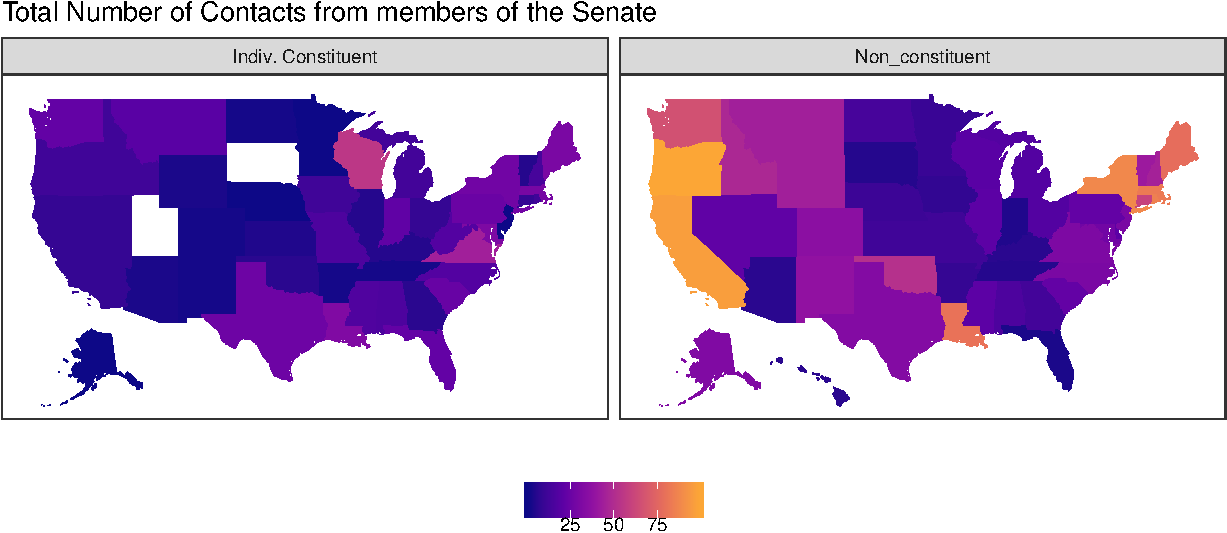
\includegraphics{Figs/sentate_percapita_map-3} \end{center}

\begin{Shaded}
\begin{Highlighting}[]
\NormalTok{d }\OperatorTok{%>%}\StringTok{ }
\StringTok{  }\KeywordTok{filter}\NormalTok{(chamber }\OperatorTok{==}\StringTok{ }\NormalTok{Chamber) }\OperatorTok{%>%}
\StringTok{  }\KeywordTok{filter}\NormalTok{(Constituent }\OperatorTok{!=}\StringTok{ "Not coded"}\NormalTok{) }\OperatorTok{%>%}\StringTok{ }
\StringTok{  }\KeywordTok{group_by}\NormalTok{(state, pop2010, Constituent) }\OperatorTok{%>%}\StringTok{ }\KeywordTok{summarise}\NormalTok{(}\DataTypeTok{n =} \KeywordTok{n}\NormalTok{()) }\OperatorTok{%>%}\StringTok{ }\KeywordTok{ungroup}\NormalTok{() }\OperatorTok{%>%}\StringTok{ }
\StringTok{  }\KeywordTok{mutate}\NormalTok{(}\DataTypeTok{Per_Capita =}\NormalTok{ n}\OperatorTok{/}\NormalTok{pop2010}\OperatorTok{*}\DecValTok{1000000}\NormalTok{) }\OperatorTok{%>%}\StringTok{ }
\StringTok{  }\CommentTok{# map_id creates the aesthetic mapping to the state name column in your data}
\StringTok{  }\KeywordTok{ggplot}\NormalTok{() }\OperatorTok{+}\StringTok{ }
\StringTok{  }\CommentTok{# map points to the fifty_states shape data}
\StringTok{  }\KeywordTok{geom_map}\NormalTok{(}\KeywordTok{aes}\NormalTok{(}\DataTypeTok{map_id =}\NormalTok{ state, }\DataTypeTok{fill =}\NormalTok{ Per_Capita), }\DataTypeTok{map =}\NormalTok{ fifty_states) }\OperatorTok{+}\StringTok{ }
\StringTok{  }\KeywordTok{expand_limits}\NormalTok{(}\DataTypeTok{x =}\NormalTok{ fifty_states}\OperatorTok{$}\NormalTok{long, }\DataTypeTok{y =}\NormalTok{ fifty_states}\OperatorTok{$}\NormalTok{lat) }\OperatorTok{+}
\StringTok{  }\KeywordTok{coord_map}\NormalTok{() }\OperatorTok{+}
\StringTok{  }\KeywordTok{scale_x_continuous}\NormalTok{(}\DataTypeTok{breaks =} \OtherTok{NULL}\NormalTok{) }\OperatorTok{+}
\StringTok{  }\KeywordTok{scale_y_continuous}\NormalTok{(}\DataTypeTok{breaks =} \OtherTok{NULL}\NormalTok{) }\OperatorTok{+}
\StringTok{  }\KeywordTok{labs}\NormalTok{(}\DataTypeTok{x =} \StringTok{""}\NormalTok{, }\DataTypeTok{y =} \StringTok{""}\NormalTok{, }\DataTypeTok{title =} \KeywordTok{paste}\NormalTok{(}\StringTok{"Contacts Per Million Residents from Members of the"}\NormalTok{, Chamber)) }\OperatorTok{+}
\StringTok{  }\KeywordTok{scale_fill_viridis_c}\NormalTok{(}\DataTypeTok{option =} \StringTok{"C"}\NormalTok{, }\DataTypeTok{end =}\NormalTok{ .}\DecValTok{8}\NormalTok{) }\OperatorTok{+}
\StringTok{  }\KeywordTok{theme}\NormalTok{(}\DataTypeTok{legend.position =} \StringTok{"bottom"}\NormalTok{, }
        \DataTypeTok{legend.title =} \KeywordTok{element_blank}\NormalTok{() )}\OperatorTok{+}
\StringTok{  }\KeywordTok{facet_grid}\NormalTok{(. }\OperatorTok{~}\StringTok{ }\NormalTok{Constituent)}
\end{Highlighting}
\end{Shaded}

\begin{center}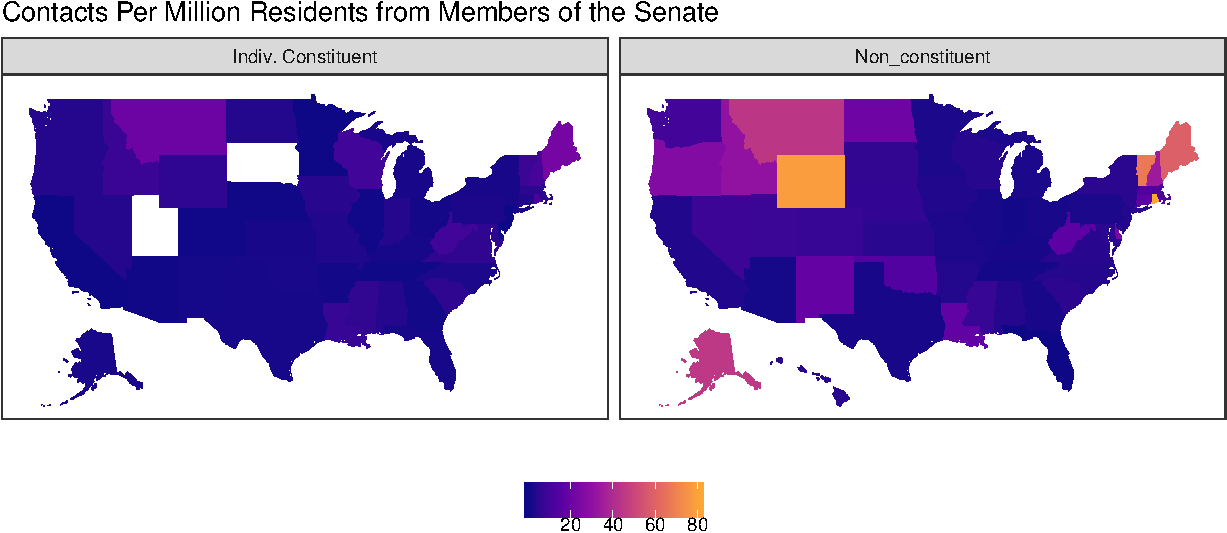
\includegraphics{Figs/sentate_percapita_map-4} \end{center}

\begin{center}\rule{0.5\linewidth}{\linethickness}\end{center}

\subsubsection{Members who contact FERC more than
average:}\label{members-who-contact-ferc-more-than-average}

\begin{Shaded}
\begin{Highlighting}[]
\CommentTok{# barcode plot of committee members }
 
\CommentTok{# member by year by agency }
\NormalTok{d }\OperatorTok{%>%}\StringTok{ }
\StringTok{  }\KeywordTok{filter}\NormalTok{(chamber }\OperatorTok{==}\StringTok{ }\NormalTok{Chamber) }\OperatorTok{%>%}\StringTok{ }
\StringTok{  }\KeywordTok{group_by}\NormalTok{(name_state) }\OperatorTok{%>%}\StringTok{ }\KeywordTok{mutate}\NormalTok{(}\DataTypeTok{n =} \KeywordTok{n}\NormalTok{()) }\OperatorTok{%>%}\StringTok{ }\KeywordTok{ungroup}\NormalTok{() }\OperatorTok{%>%}\StringTok{ }
\StringTok{  }\KeywordTok{filter}\NormalTok{(n }\OperatorTok{>}\StringTok{ }\KeywordTok{mean}\NormalTok{(n)) }\OperatorTok{%>%}
\StringTok{  }\KeywordTok{ggplot}\NormalTok{() }\OperatorTok{+}
\StringTok{  }\KeywordTok{geom_point}\NormalTok{(}
    \KeywordTok{aes}\NormalTok{(}\DataTypeTok{x =}\NormalTok{ DATE, }
        \DataTypeTok{y =} \KeywordTok{reorder}\NormalTok{(name_state, n) ), }
    \CommentTok{# alpha = .6,}
    \DataTypeTok{shape =} \DecValTok{73}\NormalTok{,}
    \DataTypeTok{size=}\DecValTok{2}
\NormalTok{  ) }\OperatorTok{+}\StringTok{  }
\StringTok{  }\KeywordTok{labs}\NormalTok{(}\DataTypeTok{title =} \KeywordTok{paste}\NormalTok{(Chamber),}
       \DataTypeTok{y =} \KeywordTok{paste}\NormalTok{(}\StringTok{"Members by"}\NormalTok{, }\StringTok{"Total Number of Letters"}\NormalTok{), }
       \DataTypeTok{x =} \StringTok{"Date of Correspondence"}\NormalTok{ ) }\OperatorTok{+}
\StringTok{  }\KeywordTok{theme}\NormalTok{(}
    \DataTypeTok{legend.title =} \KeywordTok{element_blank}\NormalTok{(),}
    \DataTypeTok{axis.text.y =} \KeywordTok{element_text}\NormalTok{(}\DataTypeTok{size=}\DecValTok{5}\NormalTok{)}
\NormalTok{  ) }\OperatorTok{+}\StringTok{ }
\StringTok{    }\KeywordTok{guides}\NormalTok{(}\DataTypeTok{fill=}\KeywordTok{guide_legend}\NormalTok{(}\DataTypeTok{ncol=}\DecValTok{1}\NormalTok{)) }
\end{Highlighting}
\end{Shaded}

\begin{center}
\includegraphics{Figs/members_barcoded-1} \end{center}

\begin{Shaded}
\begin{Highlighting}[]
\NormalTok{Chamber <-}\StringTok{ "House"} \CommentTok{# "House" #  }
 
\CommentTok{# member by year by agency }
\NormalTok{d }\OperatorTok{%>%}\StringTok{ }
\StringTok{  }\KeywordTok{filter}\NormalTok{(chamber }\OperatorTok{==}\StringTok{ }\NormalTok{Chamber) }\OperatorTok{%>%}\StringTok{ }
\StringTok{  }\KeywordTok{group_by}\NormalTok{(name_state) }\OperatorTok{%>%}\StringTok{ }\KeywordTok{mutate}\NormalTok{(}\DataTypeTok{n =} \KeywordTok{n}\NormalTok{()) }\OperatorTok{%>%}\StringTok{ }\KeywordTok{ungroup}\NormalTok{() }\OperatorTok{%>%}\StringTok{ }
\StringTok{  }\KeywordTok{filter}\NormalTok{(n }\OperatorTok{>}\StringTok{ }\KeywordTok{mean}\NormalTok{(n)) }\OperatorTok{%>%}
\StringTok{  }\KeywordTok{ggplot}\NormalTok{() }\OperatorTok{+}
\StringTok{  }\KeywordTok{geom_point}\NormalTok{(}
    \KeywordTok{aes}\NormalTok{(}\DataTypeTok{x =}\NormalTok{ DATE, }
        \DataTypeTok{y =} \KeywordTok{reorder}\NormalTok{(name_state, n) ), }
    \CommentTok{# alpha = .6,}
    \DataTypeTok{shape =} \DecValTok{73}\NormalTok{,}
    \DataTypeTok{size=}\DecValTok{2}
\NormalTok{  ) }\OperatorTok{+}\StringTok{  }
\StringTok{  }\KeywordTok{labs}\NormalTok{(}\DataTypeTok{title =} \KeywordTok{paste}\NormalTok{(Chamber),}
       \DataTypeTok{y =} \KeywordTok{paste}\NormalTok{(}\StringTok{"Members by"}\NormalTok{, }\StringTok{"Total Number of Letters"}\NormalTok{), }
       \DataTypeTok{x =} \StringTok{"Date of Correspondence"}\NormalTok{ ) }\OperatorTok{+}
\StringTok{  }\KeywordTok{theme}\NormalTok{(}
    \DataTypeTok{legend.title =} \KeywordTok{element_blank}\NormalTok{(),}
    \DataTypeTok{axis.text.y =} \KeywordTok{element_text}\NormalTok{(}\DataTypeTok{size=}\DecValTok{5}\NormalTok{)}
\NormalTok{  ) }\OperatorTok{+}\StringTok{ }
\StringTok{    }\KeywordTok{guides}\NormalTok{(}\DataTypeTok{fill=}\KeywordTok{guide_legend}\NormalTok{(}\DataTypeTok{ncol=}\DecValTok{1}\NormalTok{)) }
\end{Highlighting}
\end{Shaded}

\begin{center}
\includegraphics{Figs/members_barcoded-2} \end{center}

\subsubsection{Members who contact FERC more, relative to other
agencies:}\label{members-who-contact-ferc-more-relative-to-other-agencies}

\begin{Shaded}
\begin{Highlighting}[]
\NormalTok{all_contacts }\OperatorTok{%>%}
\StringTok{  }\KeywordTok{mutate}\NormalTok{(}\DataTypeTok{FERC =}\NormalTok{ agency }\OperatorTok{==}\StringTok{ "DOE_FERC"}\NormalTok{) }\OperatorTok{%>%}
\StringTok{  }\KeywordTok{group_by}\NormalTok{(chamber, FERC, name_state, state) }\OperatorTok{%>%}
\StringTok{  }\KeywordTok{summarise}\NormalTok{(}\DataTypeTok{n =} \KeywordTok{n}\NormalTok{() ) }\OperatorTok{%>%}
\StringTok{  }\KeywordTok{ungroup}\NormalTok{() }\OperatorTok{%>%}
\StringTok{  }\KeywordTok{spread}\NormalTok{(}\DataTypeTok{key =} \StringTok{"FERC"}\NormalTok{, }\DataTypeTok{value =} \StringTok{"n"}\NormalTok{) }\OperatorTok{%>%}\StringTok{ }
\StringTok{  }\KeywordTok{mutate}\NormalTok{(}\DataTypeTok{ShareToFERC =} \KeywordTok{round}\NormalTok{(}\StringTok{`}\DataTypeTok{TRUE}\StringTok{`}\OperatorTok{/}\NormalTok{(}\StringTok{`}\DataTypeTok{TRUE}\StringTok{`}\OperatorTok{+}\StringTok{`}\DataTypeTok{FALSE}\StringTok{`}\NormalTok{),}\DecValTok{2}\NormalTok{) )}\OperatorTok{%>%}\StringTok{ }
\StringTok{  }\KeywordTok{arrange}\NormalTok{(}\OperatorTok{-}\NormalTok{ShareToFERC) }\OperatorTok{%>%}\StringTok{ }
\StringTok{  }\KeywordTok{mutate}\NormalTok{(}\DataTypeTok{total =} \StringTok{`}\DataTypeTok{TRUE}\StringTok{`} \OperatorTok{+}\StringTok{ `}\DataTypeTok{FALSE}\StringTok{`}\NormalTok{) }\OperatorTok{%>%}\StringTok{ }
\StringTok{  }\KeywordTok{select}\NormalTok{(name_state, chamber, total, ShareToFERC) }\OperatorTok{%>%}\StringTok{ }
\StringTok{  }\KeywordTok{filter}\NormalTok{(ShareToFERC}\OperatorTok{>}\NormalTok{.}\DecValTok{3}\NormalTok{) }\OperatorTok{%>%}
\StringTok{  }\NormalTok{knitr}\OperatorTok{::}\KeywordTok{kable}\NormalTok{()}
\end{Highlighting}
\end{Shaded}

\begin{longtable}[]{@{}llrr@{}}
\toprule
name\_state & chamber & total & ShareToFERC\tabularnewline
\midrule
\endhead
MEEHAN, Martin Thomas (D) - MA & House & 8 & 0.75\tabularnewline
MOONEY, Alex X. (R) - WV & House & 46 & 0.70\tabularnewline
GOODE, Virgil H., Jr. (R) - VA & House & 239 & 0.67\tabularnewline
NORWOOD, Charles W., Jr. (R) - GA & House & 3 & 0.67\tabularnewline
JOHNSON, Mike (R) - LA & House & 22 & 0.64\tabularnewline
THOMAS, Craig Lyle (R) - WY & Senate & 15 & 0.60\tabularnewline
HIGGINS, Clay (R) - LA & House & 19 & 0.53\tabularnewline
KENNEDY, John Neely (R) - LA & Senate & 19 & 0.53\tabularnewline
PORTER, Jon C. (R) - NV & House & 19 & 0.47\tabularnewline
GARRETT, Thomas Alexander Jr. (R) - VA & House & 13 &
0.46\tabularnewline
WELLER, Gerald C. (Jerry) (R) - IL & House & 9 & 0.44\tabularnewline
NORMAN, Ralph (R) - SC & House & 7 & 0.43\tabularnewline
ALLEN, Thomas H. (D) - ME & House & 48 & 0.40\tabularnewline
McCRERY, James O., III (R) - LA & House & 47 & 0.34\tabularnewline
WU, David (D) - OR & House & 116 & 0.34\tabularnewline
ARRINGTON, Jodey Cook (R) - TX & House & 6 & 0.33\tabularnewline
DOOLITTLE, John Taylor (R) - CA & House & 18 & 0.33\tabularnewline
LEWIS, Jason Mark (R) - MN & House & 9 & 0.33\tabularnewline
SMUCKER, Lloyd K. (R) - PA & House & 18 & 0.33\tabularnewline
WICKER, Roger F. (R) - MS & House & 3 & 0.33\tabularnewline
BAIRD, Brian (D) - WA & House & 84 & 0.31\tabularnewline
KUSTER, Ann McLane (D) - NH & House & 65 & 0.31\tabularnewline
\bottomrule
\end{longtable}

\subsubsection{Members who contact FERC more in a Congress, relative to
other
agencies:}\label{members-who-contact-ferc-more-in-a-congress-relative-to-other-agencies}

\begin{Shaded}
\begin{Highlighting}[]
\NormalTok{all_contacts }\OperatorTok{%>%}
\StringTok{  }\KeywordTok{mutate}\NormalTok{(}\DataTypeTok{FERC =}\NormalTok{ agency }\OperatorTok{==}\StringTok{ "DOE_FERC"}\NormalTok{) }\OperatorTok{%>%}
\StringTok{  }\KeywordTok{group_by}\NormalTok{(congress, chamber, committees, FERC, name_state, state) }\OperatorTok{%>%}
\StringTok{  }\KeywordTok{summarise}\NormalTok{(}\DataTypeTok{n =} \KeywordTok{n}\NormalTok{() ) }\OperatorTok{%>%}
\StringTok{  }\KeywordTok{ungroup}\NormalTok{() }\OperatorTok{%>%}
\StringTok{  }\KeywordTok{spread}\NormalTok{(}\DataTypeTok{key =} \StringTok{"FERC"}\NormalTok{, }\DataTypeTok{value =} \StringTok{"n"}\NormalTok{) }\OperatorTok{%>%}\StringTok{ }
\StringTok{  }\KeywordTok{mutate}\NormalTok{(}\DataTypeTok{ShareToFERC =} \KeywordTok{round}\NormalTok{(}\StringTok{`}\DataTypeTok{TRUE}\StringTok{`}\OperatorTok{/}\NormalTok{(}\StringTok{`}\DataTypeTok{TRUE}\StringTok{`}\OperatorTok{+}\StringTok{`}\DataTypeTok{FALSE}\StringTok{`}\NormalTok{),}\DecValTok{2}\NormalTok{) )}\OperatorTok{%>%}\StringTok{ }
\StringTok{  }\KeywordTok{arrange}\NormalTok{(}\OperatorTok{-}\NormalTok{ShareToFERC) }\OperatorTok{%>%}\StringTok{ }
\StringTok{  }\KeywordTok{mutate}\NormalTok{(}\DataTypeTok{total =} \StringTok{`}\DataTypeTok{TRUE}\StringTok{`} \OperatorTok{+}\StringTok{ `}\DataTypeTok{FALSE}\StringTok{`}\NormalTok{) }\OperatorTok{%>%}\StringTok{ }
\StringTok{  }\KeywordTok{select}\NormalTok{(name_state, congress, chamber, committees, total, ShareToFERC) }\OperatorTok{%>%}\StringTok{ }
\StringTok{  }\KeywordTok{filter}\NormalTok{(ShareToFERC}\OperatorTok{>}\NormalTok{.}\DecValTok{5}\NormalTok{) }\OperatorTok{%>%}
\StringTok{  }\NormalTok{knitr}\OperatorTok{::}\KeywordTok{kable}\NormalTok{()}
\end{Highlighting}
\end{Shaded}

\begin{longtable}[]{@{}lrllrr@{}}
\toprule
name\_state & congress & chamber & committees & total &
ShareToFERC\tabularnewline
\midrule
\endhead
MOONEY, Alex X. (R) - WV & 115 & House & FINANCIAL SERVICES & 29 &
0.90\tabularnewline
GIBBS, Bob (R) - OH & 115 & House & AGRICULTURE\textbar{}TRANSPORTATION
& 9 & 0.78\tabularnewline
OLSON, Pete (R) - TX & 115 & House & ENERGY & 22 & 0.73\tabularnewline
KUSTER, Ann McLane (D) - NH & 115 & House &
AGRICULTURE\textbar{}VETERANS & 9 & 0.67\tabularnewline
JOHNSON, Mike (R) - LA & 115 & House & JUDICIARY\textbar{}NATURAL
RESOURCES & 22 & 0.64\tabularnewline
McKINLEY, David (R) - WV & 115 & House & ENERGY & 21 &
0.62\tabularnewline
CRAMER, Kevin (R) - ND & 115 & House & ENERGY & 15 & 0.60\tabularnewline
WHITEHOUSE, Sheldon (D) - RI & 115 & Senate &
BUDGET\textbar{}ENVIRONMENT\textbar{}JUDICIARY\textbar{}HEALTH\textbar{}AGING
& 30 & 0.60\tabularnewline
LYNCH, Stephen F. (D) - MA & 114 & House & FINANCIAL
SERVICES\textbar{}OVERSIGHT & 40 & 0.57\tabularnewline
WU, David (D) - OR & 110 & House &
EDUCATION\textbar{}FOREIGN\textbar{}SCIENCE & 54 & 0.56\tabularnewline
UPTON, Frederick Stephen (R) - MI & 115 & House & ENERGY & 17 &
0.53\tabularnewline
HIGGINS, Clay (R) - LA & 115 & House & HOMELAND
SECURITY\textbar{}SCIENCE\textbar{}VETERANS & 19 & 0.53\tabularnewline
KENNEDY, John Neely (R) - LA & 115 & Senate &
APPROPRIATIONS\textbar{}BANKING\textbar{}BUDGET\textbar{}JUDICIARY\textbar{}SMALL
BUSINESS & 19 & 0.53\tabularnewline
MARKEY, Edward John (D) - MA & 115 & Senate &
COMMERCE\textbar{}ENVIRONMENT\textbar{}FOREIGN RELATIONS\textbar{}SMALL
BUSINESS & 38 & 0.53\tabularnewline
\bottomrule
\end{longtable}

\subsection{Interesting cases}\label{interesting-cases}

In an article titled ``Republican congressmen's funding dwarfs
challengers''', the Charleston Gazee-Mail noted how energy companies
backed Representative Alex Mooney (R-WV). Indeed, Mooney wrote to FERC
more than any other agency, always on behalf of energy projects, mostly
pipelines. In 2017, he wrote on behalf of the Dominion Energy Supply
Header Project, National Fuel Gas Distribution Corporation's
\href{https://www.natfuel.com/supply/NorthernAccess2016/default.aspx}{Northern
Access Project}, Transcontinental Gas Pipe Line Company's
\href{https://blog.williams.com/projects-and-operations/atlantic-sunrise/atlantic-sunrise-project-placed-into-full-service/}{Atlantic
Sunrise Project}, Columbia Gas Transmission's proposed Eastern Panhandle
Expansion project, Columbia's WB Xpress Project to build new compressor
stations, In 2015 he wrote on behalf of the Columbia s Mountaineer
XPress Project, Atlantic Coast Pipeline ACP project. The parent
companies of these projects spend millions of dollars on lobbying
(Lobbyview). The WV Gazette reports funding from Dominion that is not
included in Lobbyview totals.

\begin{center}\rule{0.5\linewidth}{\linethickness}\end{center}

\subsection{Committee Leadership}\label{committee-leadership}

\begin{Shaded}
\begin{Highlighting}[]
\NormalTok{dcommittees }\OperatorTok{%>%}\StringTok{  }
\StringTok{  }\KeywordTok{mutate}\NormalTok{(}\DataTypeTok{chair =} \KeywordTok{str_remove}\NormalTok{(chair,}\StringTok{"[0-9]* |^NA "}\NormalTok{),}
         \DataTypeTok{committee =} \KeywordTok{paste}\NormalTok{(chamber, committee))}\OperatorTok{%>%}\StringTok{ }
\StringTok{  }\KeywordTok{select}\NormalTok{(committee, position, chair, chair_since_}\DecValTok{2007}\NormalTok{, DATE, assigneddate, terminationdate) }\OperatorTok{%>%}\StringTok{ }
\StringTok{  }\KeywordTok{distinct}\NormalTok{() }\OperatorTok{%>%}\StringTok{ }
\StringTok{  }\KeywordTok{filter}\NormalTok{(}\KeywordTok{str_detect}\NormalTok{(committee, }\StringTok{"ENERGY$|ENVIRONMENT|NATURAL"}\NormalTok{)) }\OperatorTok{%>%}\StringTok{ }
\StringTok{  }\KeywordTok{mutate}\NormalTok{(}\DataTypeTok{position =} \KeywordTok{ifelse}\NormalTok{(position }\OperatorTok{==}\StringTok{ "Other"}\NormalTok{, }\OtherTok{NA}\NormalTok{, position)) }\OperatorTok{%>%}
\StringTok{  }\KeywordTok{filter}\NormalTok{(}\CommentTok{# !is.na(position),}
\NormalTok{         chair_since_}\DecValTok{2007} \OperatorTok{==}\StringTok{ }\NormalTok{T) }\OperatorTok{%>%}
\StringTok{  }\KeywordTok{select}\NormalTok{(DATE, chair, position, assigneddate, terminationdate, committee) }\OperatorTok{%>%}\StringTok{ }
\StringTok{  }\KeywordTok{distinct}\NormalTok{() }\OperatorTok{%>%}\StringTok{ }
\StringTok{  }\KeywordTok{ggplot}\NormalTok{() }\OperatorTok{+}
\StringTok{  }\KeywordTok{geom_point}\NormalTok{(}
    \KeywordTok{aes}\NormalTok{(}\DataTypeTok{x =}\NormalTok{ DATE, }
        \DataTypeTok{y =}\NormalTok{ chair),}
    \DataTypeTok{shape =} \DecValTok{73}\NormalTok{,}
    \DataTypeTok{size=}\DecValTok{2} 
\NormalTok{  ) }\OperatorTok{+}
\StringTok{  }\KeywordTok{geom_segment}\NormalTok{(}\KeywordTok{aes}\NormalTok{(}\DataTypeTok{y =}\NormalTok{ chair, }\DataTypeTok{yend =}\NormalTok{ chair, }
                   \DataTypeTok{x =}\NormalTok{ assigneddate, }\DataTypeTok{xend =}\NormalTok{ terminationdate, }
                   \DataTypeTok{linetype =} \KeywordTok{factor}\NormalTok{(position)),}
               \DataTypeTok{position =} \KeywordTok{position_nudge}\NormalTok{(}\DataTypeTok{y =} \OperatorTok{-}\FloatTok{0.3}\NormalTok{)) }\OperatorTok{+}
\StringTok{  }\KeywordTok{labs}\NormalTok{(}\DataTypeTok{title =} \KeywordTok{paste}\NormalTok{(}\StringTok{"Letters to FERC from Committee Leadership"}\NormalTok{),}
       \DataTypeTok{y =} \StringTok{""}\NormalTok{, }
       \DataTypeTok{x =} \StringTok{""}\NormalTok{,}
       \DataTypeTok{linetype =} \StringTok{"Leadership position"}\NormalTok{) }\OperatorTok{+}
\StringTok{  }\KeywordTok{scale_y_discrete}\NormalTok{(}\DataTypeTok{position =} \StringTok{"right"}\NormalTok{) }\OperatorTok{+}
\StringTok{  }\KeywordTok{theme}\NormalTok{(}
    \DataTypeTok{strip.text.y =} \KeywordTok{element_text}\NormalTok{(}\DataTypeTok{angle =} \DecValTok{180}\NormalTok{, }\DataTypeTok{size =} \DecValTok{5}\NormalTok{),}
    \CommentTok{# legend.title = element_blank(),}
    \DataTypeTok{axis.text.y =} \KeywordTok{element_text}\NormalTok{(}\DataTypeTok{size=}\DecValTok{5}\NormalTok{),}
    \DataTypeTok{axis.text.x =} \KeywordTok{element_text}\NormalTok{(}\DataTypeTok{angle =} \DecValTok{0}\NormalTok{)}
\NormalTok{  ) }\OperatorTok{+}\StringTok{ }
\StringTok{  }\KeywordTok{facet_grid}\NormalTok{(committee }\OperatorTok{~}\StringTok{ }\NormalTok{., }\DataTypeTok{scales =} \StringTok{"free_y"}\NormalTok{, }\DataTypeTok{space =} \StringTok{"free_y"}\NormalTok{, }\DataTypeTok{switch =} \StringTok{"both"}\NormalTok{) }
\end{Highlighting}
\end{Shaded}

\begin{center}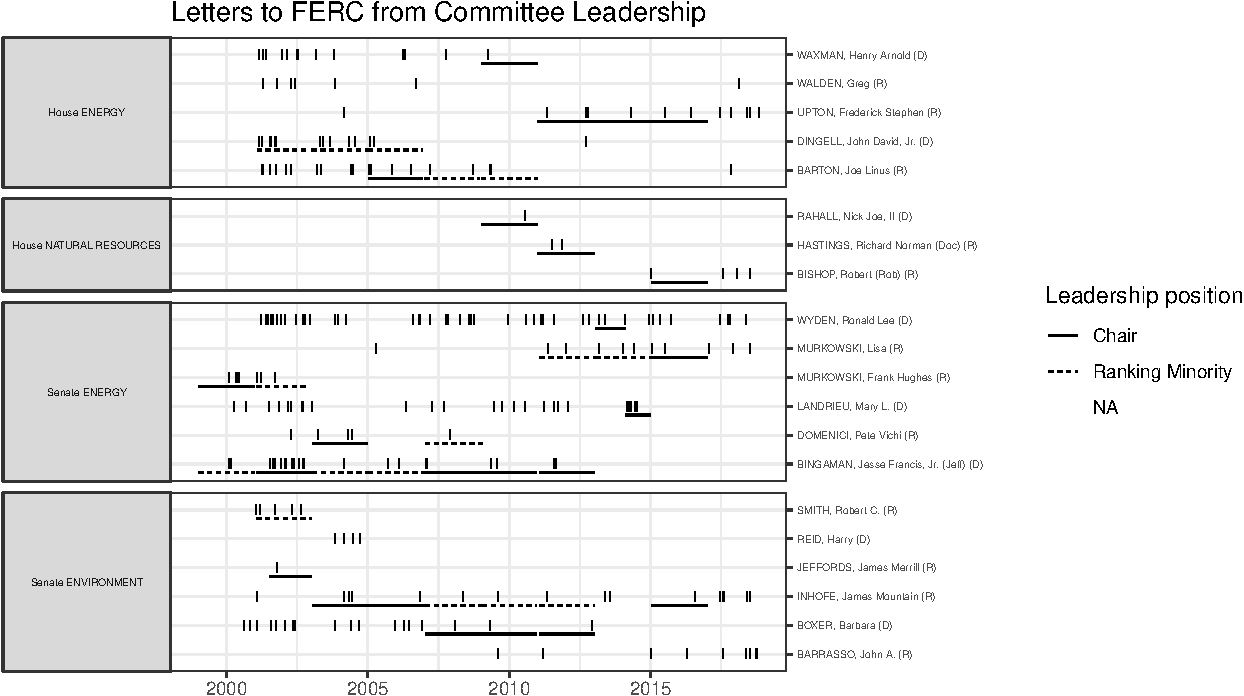
\includegraphics{Figs/committeechiars_barcode-1} \end{center}

\subsection{Many letters to FERC are
cosigned}\label{many-letters-to-ferc-are-cosigned}

\begin{Shaded}
\begin{Highlighting}[]
\CommentTok{#A rough under-estimate based on whether "et al" or "&" appears in the summary:}

\NormalTok{FERC_letters }\OperatorTok{%>%}\StringTok{ }
\StringTok{  }\KeywordTok{filter}\NormalTok{(year}\OperatorTok{>}\DecValTok{1999}\NormalTok{,}
\NormalTok{         year}\OperatorTok{<}\DecValTok{2019}\NormalTok{) }\OperatorTok{%>%}\StringTok{ }
\StringTok{  }\KeywordTok{group_by}\NormalTok{(ID) }\OperatorTok{%>%}\StringTok{ }
\StringTok{  }\KeywordTok{top_n}\NormalTok{(}\DecValTok{1}\NormalTok{) }\OperatorTok{%>%}\StringTok{ }
\StringTok{  }\KeywordTok{mutate}\NormalTok{(}\DataTypeTok{probably_cosigned =} \KeywordTok{ifelse}\NormalTok{(}\KeywordTok{str_detect}\NormalTok{(SUBJECT, }\StringTok{"et al"}\NormalTok{), }\StringTok{"et al"}\NormalTok{,}
                                 \KeywordTok{ifelse}\NormalTok{(}\KeywordTok{str_detect}\NormalTok{(SUBJECT, }\StringTok{"&"}\NormalTok{), }\StringTok{"&"}\NormalTok{, }\StringTok{" neither"}\NormalTok{))) }\OperatorTok{%>%}
\StringTok{  }\KeywordTok{group_by}\NormalTok{(year, probably_cosigned) }\OperatorTok{%>%}\StringTok{ }
\StringTok{  }\NormalTok{tally }\OperatorTok{%>%}\StringTok{ }
\StringTok{  }\KeywordTok{ggplot}\NormalTok{() }\OperatorTok{+}\StringTok{ }
\StringTok{  }\KeywordTok{aes}\NormalTok{(}\DataTypeTok{x =}\NormalTok{ year, }\DataTypeTok{y =}\NormalTok{ n, }\DataTypeTok{fill =}\NormalTok{ probably_cosigned) }\OperatorTok{+}
\StringTok{  }\KeywordTok{geom_col}\NormalTok{() }\OperatorTok{+}
\StringTok{  }\KeywordTok{scale_fill_viridis_d}\NormalTok{(}\DataTypeTok{option =} \StringTok{"C"}\NormalTok{, }\DataTypeTok{end =}\NormalTok{ .}\DecValTok{8}\NormalTok{)}
\end{Highlighting}
\end{Shaded}

Cosigned letters identified by coders

\begin{Shaded}
\begin{Highlighting}[]
\NormalTok{FERC_letters }\OperatorTok{%>%}\StringTok{ }
\StringTok{  }\KeywordTok{filter}\NormalTok{(}\OperatorTok{!}\KeywordTok{is.na}\NormalTok{(Freelancer),}
\NormalTok{         year}\OperatorTok{>}\DecValTok{1999}\NormalTok{,}
\NormalTok{         year}\OperatorTok{<}\DecValTok{2019}\NormalTok{) }\OperatorTok{%>%}\StringTok{ }
\StringTok{  }\KeywordTok{mutate}\NormalTok{(}\DataTypeTok{Cosigned =} \KeywordTok{ifelse}\NormalTok{(}\OperatorTok{!}\KeywordTok{is.na}\NormalTok{(Cosigned_House)}\OperatorTok{|!}\KeywordTok{is.na}\NormalTok{(Cosigned_Senate),}
\NormalTok{                                 T, F)) }\OperatorTok{%>%}
\StringTok{  }\KeywordTok{group_by}\NormalTok{(year, Cosigned) }\OperatorTok{%>%}\StringTok{ }
\StringTok{  }\NormalTok{tally }\OperatorTok{%>%}\StringTok{ }
\StringTok{  }\KeywordTok{ggplot}\NormalTok{() }\OperatorTok{+}\StringTok{ }
\StringTok{  }\KeywordTok{aes}\NormalTok{(}\DataTypeTok{x =}\NormalTok{ year, }\DataTypeTok{y =}\NormalTok{ n, }\DataTypeTok{fill =}\NormalTok{ Cosigned) }\OperatorTok{+}
\StringTok{  }\KeywordTok{geom_col}\NormalTok{() }\OperatorTok{+}
\StringTok{  }\KeywordTok{scale_fill_viridis_d}\NormalTok{(}\DataTypeTok{option =} \StringTok{"C"}\NormalTok{, }\DataTypeTok{end =}\NormalTok{ .}\DecValTok{8}\NormalTok{)}
\end{Highlighting}
\end{Shaded}

\begin{center}
\includegraphics{Figs/cosigned_coded-1} \end{center}

\begin{center}\rule{0.5\linewidth}{\linethickness}\end{center}

\section{Companies}\label{companies}

\subsection{Top companies in pro-business
letters}\label{top-companies-in-pro-business-letters}

\begin{Shaded}
\begin{Highlighting}[]
\CommentTok{# Split out to one obs per member per letter per business}
\NormalTok{dcorps <-}\StringTok{ }\NormalTok{d }\OperatorTok{%>%}
\StringTok{  }\KeywordTok{mutate}\NormalTok{(}\DataTypeTok{ProBusiness =}\NormalTok{ ProBusiness }\OperatorTok{%>%}\StringTok{ }\KeywordTok{str_split}\NormalTok{(}\StringTok{";"}\NormalTok{)) }\OperatorTok{%>%}
\StringTok{  }\KeywordTok{unnest}\NormalTok{(ProBusiness)}

\NormalTok{dcorps }\OperatorTok{%<>%}\StringTok{ }\KeywordTok{mutate}\NormalTok{(}\DataTypeTok{ProBusiness =}\NormalTok{ ProBusiness }\OperatorTok{%>%}
\StringTok{                     }\KeywordTok{str_replace}\NormalTok{(}\StringTok{"RTO"}\NormalTok{, }
                                 \StringTok{"Regional Transmission Organization"}\NormalTok{) }\OperatorTok{%>%}\StringTok{  }
\StringTok{         }\KeywordTok{str_remove_all}\NormalTok{(}\StringTok{" Company.*| }\CharTok{\textbackslash{}\textbackslash{}}\StringTok{(.*| Inc.*| LLC.*| Energy.*"}\NormalTok{) )}\OperatorTok{%>%}
\StringTok{  }\KeywordTok{mutate}\NormalTok{(}\DataTypeTok{AntiBusiness =}\NormalTok{ AntiBusiness }\OperatorTok{%>%}\StringTok{ }
\StringTok{           }\KeywordTok{str_replace}\NormalTok{(}\StringTok{"RTO"}\NormalTok{, }
                       \StringTok{"Regional Transmission Organization"}\NormalTok{) }\OperatorTok{%>%}\StringTok{  }
\StringTok{         }\KeywordTok{str_remove_all}\NormalTok{(}\StringTok{" Company.*| }\CharTok{\textbackslash{}\textbackslash{}}\StringTok{(.*| Inc.*| LLC.*| Energy.*"}\NormalTok{) )}

\NormalTok{dcorps }\OperatorTok{%>%}
\StringTok{  }\KeywordTok{filter}\NormalTok{(}\OperatorTok{!}\KeywordTok{is.na}\NormalTok{(ProBusiness),}
         \OperatorTok{!}\KeywordTok{str_detect}\NormalTok{(ProBusiness, }\StringTok{"Regional Transmission Organization"}\NormalTok{) ) }\OperatorTok{%>%}
\StringTok{  }\KeywordTok{group_by}\NormalTok{(ProBusiness) }\OperatorTok{%>%}
\StringTok{  }\KeywordTok{select}\NormalTok{(id, last_name, ProBusiness, ID) }\OperatorTok{%>%}
\StringTok{  }\KeywordTok{distinct}\NormalTok{() }\OperatorTok{%>%}
\StringTok{  }\KeywordTok{summarise}\NormalTok{( }\DataTypeTok{n =} \KeywordTok{n}\NormalTok{() , }
             \DataTypeTok{members =} \KeywordTok{str_c}\NormalTok{(}\KeywordTok{unique}\NormalTok{(last_name), }\DataTypeTok{collapse =} \StringTok{"; "}\NormalTok{),}
             \DataTypeTok{ID =} \KeywordTok{str_c}\NormalTok{(}\KeywordTok{unique}\NormalTok{(ID), }\DataTypeTok{collapse =} \StringTok{"; "}\NormalTok{)) }\OperatorTok{%>%}
\StringTok{  }\KeywordTok{filter}\NormalTok{(n}\OperatorTok{>}\KeywordTok{quantile}\NormalTok{(n,.}\DecValTok{9}\NormalTok{))}\OperatorTok{%>%}
\StringTok{  }\KeywordTok{arrange}\NormalTok{(}\OperatorTok{-}\NormalTok{n) }\OperatorTok{%>%}
\StringTok{  }\NormalTok{knitr}\OperatorTok{::}\KeywordTok{kable}\NormalTok{()}
\end{Highlighting}
\end{Shaded}

\begin{longtable}[]{@{}lrll@{}}
\toprule
ProBusiness & n & members & ID\tabularnewline
\midrule
\endhead
Jordan Cove & 25 & GRAVES; MORAN; YODER; BARRASSO; GARDNER; BENNET; LEE;
ENZI; HATCH; REID; SCHRADER; ROBERTS; LUMMIS; BUCK; COFFMAN; BISHOP;
CHAFFETZ; LOVE & 20160519-0010; 20160419-0011; 20160419-0010;
20160413-0017; 20160411-0008; 20150402-0007;
20150115-0026\tabularnewline
Duke & 24 & TILLIS; GRAHAM; CLYBURN; JONES; WILSON; FOXX; McHENRY;
MULVANEY; DUNCAN; ELLMERS; GOWDY; HOLDING; HUDSON; MEADOWS; PITTENGER;
RICE; ROUZER; WALKER; BURR; SCOTT; HELMS; BOUCHER; HOLLINGS &
20171208-0016; 20160523-0008; 20021008-0082; 20020617-0403;
20001229-0112\tabularnewline
Nevada Power & 21 & REID; BERKLEY; PORTER; HELLER; ENSIGN; GIBBONS;
CANTWELL; SMITH; WYDEN; BOXER; FEINSTEIN & 20080626-0022; 20040702-0082;
20031120-0152; 20031105-0382\tabularnewline
Cheniere & 14 & FARENTHOLD; GREEN; LANDRIEU; ALEXANDER; BOUSTANY;
MELANCON; CASSIDY; FLEMING; VITTER; CORNYN; INHOFE & 20140416-0025;
20100910-0040; 20050307-0011; 20050127-0022; 20050107-0022;
20050105-0146; 20040701-0068\tabularnewline
Grand River Dam Authority & 13 & INHOFE; MULLIN; BRIDENSTINE; LANKFORD &
20170809-0029; 20170807-0007; 20170802-0028; 20160826-0013;
20160803-0011; 20160729-0009; 20150804-0014\tabularnewline
PJM Interconnection & 13 & LAMB; GILLMOR; BOUCHER; GREENWOOD; PALLONE;
DAVIS; BROWN; EHRLICH; SAWYER; PITTS; WYNN; STRICKLAND; DOYLE &
20180511-0007; 20020102-0046\tabularnewline
Allegheny & 12 & CANTWELL; SMITH; REID; WYDEN; BOXER; FEINSTEIN &
20031120-0152; 20031105-0382\tabularnewline
BP & 12 & CANTWELL; SMITH; REID; WYDEN; BOXER; FEINSTEIN &
20031120-0152; 20031105-0382\tabularnewline
Enron Power Marketing, & 12 & CANTWELL; SMITH; REID; WYDEN; BOXER;
FEINSTEIN & 20031120-0152; 20031105-0382\tabularnewline
Morgan Stanley Capital Group & 12 & CANTWELL; SMITH; REID; WYDEN; BOXER;
FEINSTEIN & 20031120-0152; 20031105-0382\tabularnewline
Sierra Pacific power & 12 & CANTWELL; SMITH; REID; WYDEN; BOXER;
FEINSTEIN & 20031120-0152; 20031105-0382\tabularnewline
Union Electric & 11 & LUETKEMEYER; HARTZLER; CLEAVER; EMERSON; GRAVES;
AKIN; LONG; CLAY; SHIMKUS; SCHILLING; McCASKILL & 20110922-0009;
20110913-0012\tabularnewline
Denver Water & 10 & GARDNER; COFFMAN; PERLMUTTER; BENNET; DeGETTE &
20180622-0007; 20180411-0024; 20170404-0473\tabularnewline
Florida Gas Transmission & 9 & SHELBY; CALLAHAN; SESSIONS &
20020117-0096; 20020102-0239; 20020102-0086\tabularnewline
Wisconsin's business, & 9 & GREEN; OBEY; SENSENBRENNER; PETRI; KIND;
RYAN; BALDWIN; KOHL; FEINGOLD & 20040318-0001\tabularnewline
California Independent System Operator & 8 & OSE & 20020204-0160;
20011221-0264; 20011221-0259; 20011019-0074; 20011011-0121;
20011005-0027; 20011005-0019; 20011005-0005\tabularnewline
Columbia Gas Transmission & 8 & MOONEY; STIVERS; JENKINS; CAPITO;
McKINLEY & 20170615-0007; 20160506-0033; 20160315-0013; 20160119-0008;
20151103-0008; 20151103-0007\tabularnewline
ISO New England & 8 & REED; LEAHY; DODD; KERRY; LIEBERMAN; CHAFEE;
JEFFORDS; KENNEDY & 20011019-0270\tabularnewline
PacifiCorp & 7 & HUFFMAN; BAIRD; WU; BLUMENAUER; HOOLEY; SMITH &
20161018-0008; 20011019-0492; 20000301-0117\tabularnewline
Woodland Pulp & 7 & KING; POLIQUIN; COLLINS & 20180227-0006;
20180209-0006; 20170912-0089\tabularnewline
Hydro Renewable & 6 & SHAHEEN; KUSTER; SHEA-PORTER & 20170621-0008;
20170404-0472\tabularnewline
NRG McClain & 6 & NICKLES; INHOFE & 20040525-0113; 20040511-0052;
20040511-0051\tabularnewline
PPL Montana & 6 & BAUCUS; REHBERG; TESTER & 20071003-0168;
20071001-0199\tabularnewline
South Carolins Electric and Gas & 6 & HOLLINGS; BROWN; CLYBURN; GRAHAM;
SPENCE; SPRATT & 20010709-0250\tabularnewline
Spectra & 6 & LYNCH; ENGEL; GIBBS; JOHNSON; SIRES; GRIMM &
20160602-0013; 20151223-0021; 20150302-0021; 20131009-0016;
20120210-0001; 20120113-0002\tabularnewline
Cheyenne Plains Gas Pipeline & 5 & CUBIN; THOMAS; MUSGRAVE; ALLARD;
MORAN & 20031120-0105; 20031030-0046; 20031010-0098;
20031010-0079\tabularnewline
City of Hamilton & 5 & BROWN; VOINOVICH; SCHMIDT; BOEHNER &
20070507-0107; 20060810-0070; 20060802-0124; 20060725-0049;
20060714-0019\tabularnewline
Congressional Black Caucus & 5 & JOHNSON; RANGEL; TOWNS; OWENS; MEEKS &
20020102-0089\tabularnewline
Eastern Shore Natural Gas & 5 & CARPER; COONS; CARNEY & 20171004-0007;
20160621-0020\tabularnewline
Kinder Morgan & 5 & SHAHEEN; KUSTER; GUINTA; AYOTTE; COCHRAN &
20150204-0011; 20141229-0090\tabularnewline
Magnolia LNG & 5 & BOUSTANY; CASSIDY; VITTER & 20160222-0007;
20160209-0024; 20160129-0008; 20150320-0022;
20150311-0010\tabularnewline
Straight Creek Gathering, LP & 5 & ROGERS & 20061006-0193;
20061006-0191; 20060628-0147; 20060622-0084;
20060621-0127\tabularnewline
Tellurian & 5 & HIGGINS; SCALISE; CASSIDY; GREEN; GONZALEZ &
20181109-0007; 20181105-0012; 20181105-0011\tabularnewline
\bottomrule
\end{longtable}

\subsection{Letters citing companies registered with
FERC}\label{letters-citing-companies-registered-with-ferc}

Of the companies registered to interact with FERC, several appear in the
letter texts. Here \texttt{company\_short} is a shortened version a name
that refrences several affiliated companies, each of which are
registered separatly. \emph{TO DO:}

\begin{itemize}
\item
  \begin{enumerate}
  \def\labelenumi{(\arabic{enumi})}
  \tightlist
  \item
    Identify linked corporations for other top companies in the data
    using
    \href{https://docs.google.com/spreadsheets/d/1FjZIuz8T97nczCbYskjT7-Hl6we6hoa6VndOnFmKDGU/edit\#gid=0}{this
    sheet}
  \end{enumerate}
\item
  \begin{enumerate}
  \def\labelenumi{(\arabic{enumi})}
  \setcounter{enumi}{1}
  \tightlist
  \item
    extract company contact persons and information from the FERC
    website.
  \end{enumerate}
\end{itemize}

\begin{Shaded}
\begin{Highlighting}[]
\KeywordTok{load}\NormalTok{(}\KeywordTok{here}\NormalTok{(}\StringTok{"data"}\NormalTok{, }\StringTok{"DOE_FERC-corps.Rdata"}\NormalTok{))}
\NormalTok{FERC_corps }\OperatorTok{%<>%}\StringTok{ }\KeywordTok{ungroup}\NormalTok{() }\OperatorTok{%>%}\StringTok{ }\KeywordTok{group_by}\NormalTok{(company_short) }\OperatorTok{%>%}\StringTok{ }\KeywordTok{mutate}\NormalTok{(}\DataTypeTok{industry =} \KeywordTok{str_c}\NormalTok{(}\KeywordTok{unique}\NormalTok{(industry), }\DataTypeTok{collapse =} \StringTok{";"}\NormalTok{)) }\OperatorTok{%>%}\StringTok{ }\KeywordTok{select}\NormalTok{(}\OperatorTok{-}\NormalTok{company, }\OperatorTok{-}\NormalTok{Fortune500) }\OperatorTok{%>%}\StringTok{ }\KeywordTok{distinct}\NormalTok{() }

\NormalTok{## Make a single string of short corp names}
\NormalTok{ferc_short <-}\StringTok{ }\KeywordTok{unique}\NormalTok{(FERC_corps}\OperatorTok{$}\NormalTok{company_short) }\OperatorTok{%>%}\StringTok{ }
\StringTok{  }\KeywordTok{str_c}\NormalTok{(}\DataTypeTok{collapse =} \StringTok{"|"}\NormalTok{) }\OperatorTok{%>%}\StringTok{ }
\StringTok{  }\KeywordTok{str_remove_all}\NormalTok{(}\StringTok{"||"}\NormalTok{)}

\CommentTok{# bad string? }
\CommentTok{# str_detect("", ferc_short)}

\KeywordTok{save}\NormalTok{(ferc_short, }\DataTypeTok{file =} \KeywordTok{here}\NormalTok{(}\StringTok{"data/ferc_short.Rdata"}\NormalTok{))}
\end{Highlighting}
\end{Shaded}

\subsection{Pro-business letters}\label{pro-business-letters}

\begin{Shaded}
\begin{Highlighting}[]
\NormalTok{dcorps }\OperatorTok{%>%}
\StringTok{  }\KeywordTok{mutate}\NormalTok{(}\DataTypeTok{company_short =} \KeywordTok{str_extract}\NormalTok{(ProBusiness, ferc_short)) }\OperatorTok{%>%}
\StringTok{  }\KeywordTok{left_join}\NormalTok{(FERC_corps) }\OperatorTok{%>%}\StringTok{ }
\StringTok{  }\KeywordTok{distinct}\NormalTok{() }\OperatorTok{%>%}
\StringTok{  }\KeywordTok{group_by}\NormalTok{(company_short_refs) }\OperatorTok{%>%}
\StringTok{  }\KeywordTok{select}\NormalTok{(ID, last_name, company_short, company_short_refs) }\OperatorTok{%>%}
\StringTok{  }\KeywordTok{filter}\NormalTok{(company_short }\OperatorTok{!=}\StringTok{ ""}\NormalTok{)}\OperatorTok{%>%}
\StringTok{  }\KeywordTok{distinct}\NormalTok{() }\OperatorTok{%>%}
\StringTok{  }\KeywordTok{summarise}\NormalTok{( }\DataTypeTok{n =} \KeywordTok{n}\NormalTok{() , }
             \DataTypeTok{company_short =} \KeywordTok{str_c}\NormalTok{(}\KeywordTok{unique}\NormalTok{(company_short), }\DataTypeTok{collapse =} \StringTok{"; "}\NormalTok{),}
             \DataTypeTok{members =} \KeywordTok{str_c}\NormalTok{(}\KeywordTok{unique}\NormalTok{(last_name), }\DataTypeTok{collapse =} \StringTok{"; "}\NormalTok{),}
             \DataTypeTok{ID =} \KeywordTok{str_c}\NormalTok{(}\KeywordTok{unique}\NormalTok{(ID), }\DataTypeTok{collapse =} \StringTok{"; "}\NormalTok{)) }\OperatorTok{%>%}
\StringTok{  }\KeywordTok{filter}\NormalTok{(n}\OperatorTok{>}\KeywordTok{quantile}\NormalTok{(n,.}\DecValTok{9}\NormalTok{))}\OperatorTok{%>%}
\StringTok{  }\KeywordTok{select}\NormalTok{(company_short, n, }\KeywordTok{everything}\NormalTok{()) }\OperatorTok{%>%}
\StringTok{  }\KeywordTok{arrange}\NormalTok{(}\OperatorTok{-}\NormalTok{n) }\OperatorTok{%>%}
\StringTok{  }\NormalTok{knitr}\OperatorTok{::}\KeywordTok{kable}\NormalTok{()}
\end{Highlighting}
\end{Shaded}

\begin{longtable}[]{@{}lrlll@{}}
\toprule
company\_short & n & company\_short\_refs & members & ID\tabularnewline
\midrule
\endhead
Duke & 25 & Duke Energy Carolinas, LLC; Duke Energy Indiana, LLC.; Duke
Energy Progress, LLC.; Duke Energy Kentucky, Inc.; Duke Energy Ohio,
Inc.; Duke Energy Carolinas, LLC; Duke Energy Corporation; Duke Energy
Florida, Inc.; Duke Energy Indiana, Inc.; Duke Energy Kentucky, Inc.;
Duke Energy Ohio, Inc.; Duke Energy Progress, Inc.; Duke Energy Shared
Services LLC & TILLIS; GRAHAM; CLYBURN; JONES; WILSON; FOXX; McHENRY;
MULVANEY; DUNCAN; ELLMERS; GOWDY; HOLDING; HUDSON; MEADOWS; PITTENGER;
RICE; ROUZER; WALKER; BURR; SCOTT; HELMS; BOUCHER; HOLLINGS &
20171208-0016; 20160523-0008; 20060508-0029(partial); 20021008-0082;
20020617-0403; 20001229-0112\tabularnewline
Nevada Power & 22 & Nevada Power Company & REID; BERKLEY; PORTER;
HELLER; ENSIGN; GIBBONS; CANTWELL; SMITH; WYDEN; BOXER; FEINSTEIN &
20130725-0017; 20080626-0022; 20040702-0082; 20031120-0152;
20031105-0382\tabularnewline
PJM Interconnection & 13 & PJM Interconnection, L.L.C. & LAMB; GILLMOR;
BOUCHER; GREENWOOD; PALLONE; DAVIS; BROWN; EHRLICH; SAWYER; PITTS; WYNN;
STRICKLAND; DOYLE & 20180511-0007; 20020102-0046\tabularnewline
Allegheny & 12 & Allegheny Energy Service Corporation; Allegheny Energy
Supply Company, LLC; Allegheny Energy Supply Company, LLC; Allegheny
Energy Supply Units 3, 4, \& 5, LLC & CANTWELL; SMITH; REID; WYDEN;
BOXER; FEINSTEIN & 20031120-0152; 20031105-0382\tabularnewline
BP & 12 & BP Pipelines (Alaska) Inc.; BP Pipelines (North America) Inc.;
BP Energy Company; BP Energy Company & CANTWELL; SMITH; REID; WYDEN;
BOXER; FEINSTEIN & 20031120-0152; 20031105-0382\tabularnewline
Enron Power Marketing & 12 & Enron Power Marketing, Inc. & CANTWELL;
SMITH; REID; WYDEN; BOXER; FEINSTEIN & 20031120-0152;
20031105-0382\tabularnewline
ISO New England & 12 & ISO New England Inc. & REED; LEAHY; DODD; KERRY;
LIEBERMAN; CHAFEE; JEFFORDS; KENNEDY; SNOWE; BALDACCI; ALLEN; COLLINS &
20011019-0270; 20010111-0319\tabularnewline
Morgan Stanley Capital Group & 12 & Morgan Stanley Capital Group Inc. &
CANTWELL; SMITH; REID; WYDEN; BOXER; FEINSTEIN & 20031120-0152;
20031105-0382\tabularnewline
\bottomrule
\end{longtable}

\begin{Shaded}
\begin{Highlighting}[]
\NormalTok{## Longer list with company full names}
\CommentTok{# d %>%}
\CommentTok{#   mutate(company_short = str_extract(ProBusiness, ferc_short)) %>%}
\CommentTok{#   drop_na(company_short) %>%}
\CommentTok{#   mutate(members = paste(CongressPerson, Cosigned_House, Cosigned_Senate, sep = ";")) %>%}
\CommentTok{#   mutate(members = str_remove_all(members, ";NA")) %>%}
\CommentTok{#   group_by(company_short) %>%}
\CommentTok{#   mutate(members = str_c(unique(members), collapse = ";")) %>%}
\CommentTok{#   select(company_short, members) %>%  distinct() %>%}
\CommentTok{#   left_join(FERC_corps) %>% distinct() %>%}
\CommentTok{#   knitr::kable(caption = "Pro Businesses matching those registered with FERC")}
\end{Highlighting}
\end{Shaded}

\subsection{Anti-business letters}\label{anti-business-letters}

\begin{Shaded}
\begin{Highlighting}[]
\NormalTok{dcorps }\OperatorTok{%>%}
\StringTok{  }\KeywordTok{mutate}\NormalTok{(}\DataTypeTok{company_short =} \KeywordTok{str_extract}\NormalTok{(AntiBusiness, ferc_short)) }\OperatorTok{%>%}
\StringTok{  }\KeywordTok{left_join}\NormalTok{(FERC_corps) }\OperatorTok{%>%}\StringTok{ }
\StringTok{  }\KeywordTok{distinct}\NormalTok{() }\OperatorTok{%>%}
\StringTok{  }\KeywordTok{group_by}\NormalTok{(company_short_refs) }\OperatorTok{%>%}
\StringTok{  }\KeywordTok{select}\NormalTok{(ID, last_name, company_short, company_short_refs) }\OperatorTok{%>%}
\StringTok{  }\KeywordTok{filter}\NormalTok{(company_short }\OperatorTok{!=}\StringTok{ ""}\NormalTok{)}\OperatorTok{%>%}
\StringTok{  }\KeywordTok{distinct}\NormalTok{() }\OperatorTok{%>%}
\StringTok{  }\KeywordTok{summarise}\NormalTok{( }\DataTypeTok{n =} \KeywordTok{n}\NormalTok{() , }
             \DataTypeTok{company_short =} \KeywordTok{str_c}\NormalTok{(}\KeywordTok{unique}\NormalTok{(company_short), }\DataTypeTok{collapse =} \StringTok{"; "}\NormalTok{),}
             \DataTypeTok{members =} \KeywordTok{str_c}\NormalTok{(}\KeywordTok{unique}\NormalTok{(last_name), }\DataTypeTok{collapse =} \StringTok{"; "}\NormalTok{),}
             \DataTypeTok{ID =} \KeywordTok{str_c}\NormalTok{(}\KeywordTok{unique}\NormalTok{(ID), }\DataTypeTok{collapse =} \StringTok{"; "}\NormalTok{)) }\OperatorTok{%>%}
\StringTok{  }\KeywordTok{filter}\NormalTok{(n}\OperatorTok{>}\KeywordTok{quantile}\NormalTok{(n,.}\DecValTok{9}\NormalTok{))}\OperatorTok{%>%}
\StringTok{  }\KeywordTok{select}\NormalTok{(company_short, n, }\KeywordTok{everything}\NormalTok{()) }\OperatorTok{%>%}
\StringTok{  }\KeywordTok{arrange}\NormalTok{(}\OperatorTok{-}\NormalTok{n) }\OperatorTok{%>%}
\StringTok{  }\NormalTok{knitr}\OperatorTok{::}\KeywordTok{kable}\NormalTok{()}
\end{Highlighting}
\end{Shaded}

\begin{longtable}[]{@{}lrlll@{}}
\toprule
company\_short & n & company\_short\_refs & members & ID\tabularnewline
\midrule
\endhead
Dominion & 124 & Dominion Energy Cove Point LNG, LP; Dominion Energy
Questar Pipeline, LLC; Dominion Energy Overthrust Pipeline, LLC;
Dominion Energy Transmission, Inc; Dominion Energy Cove Point LNG, LP;
Dominion Energy Kewaunee, Inc.; Dominion Energy Manchester Street, Inc.;
Dominion Energy Marketing, Inc.; Dominion Energy Transmission, Inc & VAN
HOLLEN; GOODLATTE; KAINE; FORBES; GIBSON; HANNA; COCHRAN; MIKULSKI;
CARDIN; WYNN; WARNER; ROCKEFELLER; SARBANES; RAHALL; BYRD; ALLEN; GOODE;
CANTOR; BOUCHER & 20170918-0007; 20170802-0031; 20170609-0037;
20160406-0022; 20150826-0036; 20150826-0031; 20150311-0008;
20150311-0007; 20150303-0016; 20150130-0007; 20150126-0033;
20150115-0028; 20141229-0090; 20140311-0010; 20070716-0289;
20060622-0070; 20060508-0086(partial); 20060508-0085(partial);
20060215-0049; 20050415-0090; 20050401-0069; 20050127-0001;
20041118-0117; 20040907-0363; 20030423-0206; 20030305-0180;
20030123-0076; 20030123-0075; 20030123-0074; 20021023-0211;
20021001-0192; 20021001-0191; 20021001-0190; 20020930-0236;
20020930-0230; 20020930-0229; 20020930-0228; 20020930-0227;
20020930-0226; 20020930-0220; 20020926-0397; 20020924-0059;
20020919-0119; 20020910-0166; 20020910-0164; 20020909-0633;
20020909-0178; 20020823-0296; 20020815-0648; 20020815-0640;
20020813-0319; 20020813-0007; 20020716-0149; 20020716-0145;
20020716-0141; 20020716-0140; 20020702-0076; 20020702-0068;
20020702-0061; 20020625-0315; 20020625-0314; 20020625-0313;
20020625-0312; 20020625-0311; 20020625-0310; 20020625-0309;
20020621-0230; 20020617-0409; 20020610-0156; 20020610-0155;
20020610-0154; 20020610-0153; 20020610-0152; 20020610-0151;
20020610-0149; 20020610-0148; 20020610-0147; 20020610-0146;
20020610-0145; 20020610-0144; 20020610-0143; 20020610-0142;
20020610-0141; 20020524-0542; 20020521-0016; 20020521-0015;
20020521-0014; 20020521-0013; 20020521-0012; 20020521-0011;
20020521-0010; 20020509-0097; 20020423-0285; 20020423-0283;
20020423-0282; 20020423-0281; 20020423-0280; 20020423-0279;
20020423-0278; 20020423-0120; 20020423-0119; 20020423-0118;
20020423-0117; 20020423-0116; 20020423-0115; 20020423-0114;
20020423-0106; 20020403-0672; 20020403-0671; 20020403-0669;
20020403-0668; 20020403-0667; 20020403-0666; 20020403-0653;
20020403-0651; 20020403-0649; 20020318-0738; 20020315-0080;
20020311-0007; 20011010-0217; 20011005-0099; 20010806-0443;
20010709-0426\tabularnewline
Columbia Gas Transmission & 39 & Columbia Gas Transmission, LLC &
CARDIN; HOYER; CUMMINGS; SARBANES; MIKULSKI; RUPPERSBERGER; BROWN;
VOINOVICH; JORDAN; BYRD; LOWEY; GILMAN; KELLY; SCHUMER; CLINTON;
JOHNSON; RANGEL; TOWNS; OWENS; MEEKS & 20130124-0015; 20120712-0003;
20090908-0068; 20090812-0016; 20090527-0015; 20090508-0077;
20081222-0201; 20081113-0083; 20081001-0013; 20081001-0012;
20080731-0190; 20080619-0125; 20020807-3146; 20020204-0078;
20020129-0194; 20020117-0167; 20020117-0166; 20020117-0098;
20020102-0245; 20020102-0240; 20020102-0093; 20020102-0092;
20020102-0090; 20020102-0089; 20020102-0088; 20011108-0078;
20010815-0584\tabularnewline
Duke & 34 & Duke Energy Carolinas, LLC; Duke Energy Indiana, LLC.; Duke
Energy Progress, LLC.; Duke Energy Kentucky, Inc.; Duke Energy Ohio,
Inc.; Duke Energy Carolinas, LLC; Duke Energy Corporation; Duke Energy
Florida, Inc.; Duke Energy Indiana, Inc.; Duke Energy Kentucky, Inc.;
Duke Energy Ohio, Inc.; Duke Energy Progress, Inc.; Duke Energy Shared
Services LLC & McHENRY; DUNCAN; HAGAN; MYRICK; DOLE; PLATTS; DeMINT;
SPRATT; COCHRAN; GOODE; WARNER; FEINSTEIN; FRIST; LUCAS; ALLEN; BOUCHER
& 20170508-0011(partial); 20151201-0086(partial); 20110321-0050;
20110302-0023; 20101119-0024; 20100804-0015; 20100525-0030;
20100525-0021; 20080522-0130; 20080522-0129; 20071231-0079;
20061011-0271(partial); 20061010-0221; 20050520-0293; 20041018-0033;
20021206-0130; 20021206-0098; 20021018-0239; 20021008-0087;
20021008-0068; 20021008-0066; 20021008-0060; 20020923-0167;
20020813-0003; 20020730-0177; 20020520-1521; 20020503-0166;
20020423-0284; 20011004-0504; 20011004-0498; 20011002-0352;
20010709-0422; 20010709-0410; 20010703-0111\tabularnewline
ISO New England & 31 & ISO New England Inc. & MARKEY; COLLINS; GREGG;
REED; MOAKLEY; FRANK; DELAHUNT; McGOVERN; CAPUANO; MEEHAN; NEAL;
TIERNEY; KENNEDY; KERRY; SNOWE; ALLEN; BALDACCI & 20050810-0209;
20050719-0104; 20050719-0103; 20050711-0239; 20050711-0238;
20010329-0009; 20010329-0005; 20010329-0003;
20010329-0002\tabularnewline
Tennessee Gas Pipeline & 29 & Tennessee Gas Pipeline Company, L.L.C. &
MARKEY; WARREN; NEAL; COOPER; McCONNELL; KUSTER; AYOTTE; SCHUMER;
GILLIBRAND; TSONGAS; LARSON; TONKO; GIBSON; McGOVERN; CASEY; SUNUNU;
SMITH; SANTORUM & 20180111-0007; 20170428-0009; 20170421-0006;
20161014-0011; 20160926-0009; 20160624-0017; 20160510-0011;
20160510-0010; 20160405-0074; 20160309-0119; 20160212-0008;
20151020-0012; 20150908-0010; 20150908-0009; 20150902-0023;
20150715-0058; 20150518-0133; 20141107-0007; 20120712-0011;
20041123-0082; 20041115-0071; 20010709-0434; 20010709-0433;
20000828-0095\tabularnewline
Spectra & 26 & Spectra Energy Transmission, LLC & LYNCH; MARKEY; WARREN;
LOWEY; SCHUMER; GILLIBRAND; CHAMBLISS; SIRES; PLATTS; CASEY; SHUSTER;
KERRY & 20180223-0007; 20170405-0192; 20170201-0010; 20170109-0048;
20161216-0007; 20161004-0075; 20160805-0007; 20160729-0014;
20160614-0011; 20160601-0006; 20150625-0023; 20150408-0006;
20140424-0016; 20100318-0018; 20090908-0072(partial);
20080919-0123(partial); 20080731-0186(partial); 20080424-0053;
20071217-0183\tabularnewline
Transcontinental & 26 & Transcontinental Gas Pipeline Company, LLC &
PALLONE; BOOKER; MacARTHUR; HOLT; SPECTER; PITTS; GERLACH; CASEY; WEBB;
WOLF; SMITH; LAUTENBERG; CORZINE; HELMS; MYRICK; WATT & 20180516-0006;
20180326-0009; 20170829-0016; 20160926-0008; 20160301-0012;
20130625-0010; 20080929-0011; 20080919-0131; 20080820-0006;
20080310-0104; 20070402-0017; 20070312-0037; 20070308-0146;
20050329-0055; 20040528-0075; 20030813-0100; 20020117-0079;
20010806-0434; 20010806-0433; 20010627-0095; 20010622-0220;
20010329-0065; 20000911-0352\tabularnewline
Ameren & 19 & Ameren Corporation; Ameren Energy Medina Valley Cogen,
L.L.C. & BLUNT; LUETKEMEYER; McCASKILL; HULSHOF; CLAY; MOORE; BROWNBACK;
ROBERTS; SKELTON; BOND & 20180216-0016; 20110315-0013(partial);
20101006-0005(partial); 20080407-0122; 20070905-0024; 20060518-0038;
20060518-0005(partial); 20060517-0319(partial); 20060517-0317(partial);
20060517-0316; 20060508-0115(partial); 20060508-0106(partial);
20060424-0054(partial); 20060327-0069; 20060320-0113; 20060317-0013;
20060315-0165; 20060130-0019; 20051219-0393\tabularnewline
Appalachian Power & 15 & Appalachian Power Company & GARRETT; KAINE;
GRIFFITH; ROE; PERRIELLO; WARNER; GOODE & 20170613-4008(partial);
20170217-0007; 20110719-0003; 20110218-0028(partial); 20100910-0037;
20100910-0031(partial); 20100525-0023; 20091123-0150; 20091013-0008;
20080310-0107; 20040806-0024; 20030822-0325; 20030822-0160;
20030801-0191\tabularnewline
Rockies Express & 15 & Rockies Express Pipeline LLC & PENCE; TURNER;
BOEHNER; LUGAR; BAYH; HOBSON; VOINOVICH; HARE & 20090908-0069;
20090702-0125; 20090618-0095; 20080611-0154; 20080522-0154;
20080515-0182(partial); 20080512-0256; 20080411-0032;
20071107-0195(partial); 20070807-0083; 20070709-0238(partial);
20070709-0237; 20070508-0195; 20070507-0290;
20060725-0018\tabularnewline
Florida Gas Transmission & 13 & Florida Gas Transmission Company, LLC &
NELSON; CLINTON; KELLER; THURMAN & 20100910-0033(partial);
20100910-0029(partial); 20020813-0004; 20020716-0143; 20020716-0136;
20020521-0106; 20011221-0268; 20011019-0102; 20010830-0761;
20010806-0485; 20010806-0446; 20010726-0102;
20010726-0100\tabularnewline
\bottomrule
\end{longtable}

\begin{Shaded}
\begin{Highlighting}[]
\NormalTok{## Longer list with company full names}
\CommentTok{# d %>% }
\CommentTok{#   mutate(company_short = str_extract(AntiBusiness, ferc_short)) %>% }
\CommentTok{#   drop_na(company_short) %>% }
\CommentTok{#   mutate(members = paste(CongressPerson, Cosigned_House, Cosigned_Senate, sep = ";")) %>%}
\CommentTok{#   mutate(members = str_remove_all(members, ";NA")) %>% }
\CommentTok{#   group_by(company_short) %>% }
\CommentTok{#   mutate(members = str_c(unique(members), collapse = ";")) %>% }
\CommentTok{#   select(company_short, members) %>%  distinct() %>%}
\CommentTok{#   left_join(FERC_corps) %>% distinct() %>% }
\CommentTok{#   knitr::kable(caption = "Anti Businesses matching those registered with FERC")}
\end{Highlighting}
\end{Shaded}

\begin{center}\rule{0.5\linewidth}{\linethickness}\end{center}

\subsection{Company lookup table}\label{company-lookup-table}

Clean companies names extracted from letters and create shortened name
that is more likely to be found in other datasets (like done with
FERC-registerd companies above).

\begin{Shaded}
\begin{Highlighting}[]
\CommentTok{# Split out to one obs per member per letter per business}
\NormalTok{dcorps <-}\StringTok{ }\NormalTok{d }\OperatorTok{%>%}
\StringTok{  }\KeywordTok{select}\NormalTok{(ID, bioname, ProBusiness, AntiBusiness, ProProject, AntiProject) }\OperatorTok{%>%}\StringTok{ }
\StringTok{  }\KeywordTok{gather}\NormalTok{(}\DataTypeTok{value =} \StringTok{"company"}\NormalTok{, }\DataTypeTok{key =} \StringTok{"position"}\NormalTok{, }\OperatorTok{-}\NormalTok{ID, }\OperatorTok{-}\NormalTok{bioname) }\OperatorTok{%>%}
\StringTok{  }\KeywordTok{mutate}\NormalTok{(}\DataTypeTok{company =}\NormalTok{ company }\OperatorTok{%>%}\StringTok{ }\KeywordTok{str_split}\NormalTok{(}\StringTok{";"}\NormalTok{)) }\OperatorTok{%>%}
\StringTok{  }\KeywordTok{unnest}\NormalTok{(company) }\OperatorTok{%>%}\StringTok{ }\KeywordTok{distinct}\NormalTok{()}

\NormalTok{dcorps }\OperatorTok{%<>%}\StringTok{ }\KeywordTok{mutate}\NormalTok{(}\DataTypeTok{company =}\NormalTok{ company }\OperatorTok{%>%}
\StringTok{                     }\KeywordTok{str_replace}\NormalTok{(}\StringTok{"RTO"}\NormalTok{, }
                                 \StringTok{"Regional Transmission Organization"}\NormalTok{) }\OperatorTok{%>%}\StringTok{  }
\StringTok{         }\KeywordTok{str_remove_all}\NormalTok{(}\StringTok{" Company.*| }\CharTok{\textbackslash{}\textbackslash{}}\StringTok{(.*| Inc.*| LLC.*| Energy.*"}\NormalTok{) )}

\NormalTok{dcorps}\OperatorTok{$}\NormalTok{company }\OperatorTok{%<>%}
\StringTok{  }\KeywordTok{trimws}\NormalTok{()  }\CommentTok{# trim white space before and after company names}

\NormalTok{dcorps }\OperatorTok{%<>%}\StringTok{   }\KeywordTok{filter}\NormalTok{(}\KeywordTok{nchar}\NormalTok{(company)}\OperatorTok{>}\DecValTok{1}\NormalTok{) }\OperatorTok{%>%}\CommentTok{# drop names less than 1 character}
\StringTok{  }\KeywordTok{distinct}\NormalTok{() }\CommentTok{# drop duplicates}

\NormalTok{## For matching, remove endings like ", Inc." etc. }
\NormalTok{trim <-}\StringTok{ }\ControlFlowTok{function}\NormalTok{(d)\{}
\NormalTok{d }\OperatorTok{%>%}
\StringTok{  }\KeywordTok{str_remove_all}\NormalTok{(}\StringTok{"Village of |}\CharTok{\textbackslash{}\textbackslash{}}\StringTok{(.*|,.*| -.*|^Proposed | Pipe.*| pipe.*| project$| Proiects$| Company.*| Comnany| Corp.*| Co$| Co.$| Energy$| energy$| power$| Power marketing$| Holdings.*| Group$| Gas$| Project.*| LLC| L.L.C.|  L.P.|^The | Inc.| L.P.| Ltd.| LP| Limited Partnership| Limited Liability|  Facility| Transportation and Storage| Storage and Transportation"}\NormalTok{) }\OperatorTok{%>%}\StringTok{ }
\StringTok{  }\KeywordTok{str_remove_all}\NormalTok{(}\StringTok{"^, "}\NormalTok{) }\OperatorTok{%>%}
\StringTok{  }\KeywordTok{trimws}\NormalTok{()  }\CommentTok{# filter out names less than 2 characters }
\NormalTok{\}}



\NormalTok{dcorps}\OperatorTok{$}\NormalTok{company_short <-}\StringTok{ }\KeywordTok{trim}\NormalTok{(dcorps}\OperatorTok{$}\NormalTok{company) }\OperatorTok{%>%}\StringTok{ }\KeywordTok{trim}\NormalTok{()}
\end{Highlighting}
\end{Shaded}

Problem company names that may need to be fixed (e.g.~to remove special
characters or spell out abbreviated name)

\begin{Shaded}
\begin{Highlighting}[]
\CommentTok{# Problem Names}
\NormalTok{dcorps }\OperatorTok{%>%}\StringTok{ }\KeywordTok{filter}\NormalTok{(}\KeywordTok{nchar}\NormalTok{(company_short)}\OperatorTok{<}\DecValTok{2}\NormalTok{) }\OperatorTok{%>%}\StringTok{ }\NormalTok{knitr}\OperatorTok{::}\KeywordTok{kable}\NormalTok{()}
\end{Highlighting}
\end{Shaded}

\begin{longtable}[]{@{}lllll@{}}
\toprule
ID & bioname & position & company & company\_short\tabularnewline
\midrule
\endhead
\bottomrule
\end{longtable}

\begin{Shaded}
\begin{Highlighting}[]
\NormalTok{dcorps }\OperatorTok{%<>%}\StringTok{ }\KeywordTok{filter}\NormalTok{(}\KeywordTok{nchar}\NormalTok{(company_short)}\OperatorTok{>}\DecValTok{1}\NormalTok{)}
\end{Highlighting}
\end{Shaded}

Identify short names by hand:

\begin{Shaded}
\begin{Highlighting}[]
\NormalTok{## Correct over-trimmed names}
\NormalTok{dcorps }\OperatorTok{%<>%}\StringTok{ }
\StringTok{  }\KeywordTok{mutate}\NormalTok{(}\DataTypeTok{company_short =} \KeywordTok{ifelse}\NormalTok{(company }\OperatorTok{==}\StringTok{ "Columbia Energy Power Marketing Corporation"}\NormalTok{, }\StringTok{"Columbia Energy"}\NormalTok{, company_short))}\OperatorTok{%>%}
\StringTok{  }\KeywordTok{mutate}\NormalTok{(}\DataTypeTok{company_short =} \KeywordTok{ifelse}\NormalTok{(company }\OperatorTok{==}\StringTok{ "Michigan Energy Exchange, LLC"}\NormalTok{, }\StringTok{"Michigan Energy"}\NormalTok{, company_short))}\OperatorTok{%>%}
\StringTok{  }\KeywordTok{mutate}\NormalTok{(}\DataTypeTok{company_short =} \KeywordTok{ifelse}\NormalTok{(company }\OperatorTok{==}\StringTok{ "Midwest Energy, Inc."}\NormalTok{, }\StringTok{"Midwest Energy"}\NormalTok{, company_short))}\OperatorTok{%>%}
\StringTok{  }\KeywordTok{mutate}\NormalTok{(}\DataTypeTok{company_short =} \KeywordTok{ifelse}\NormalTok{(company }\OperatorTok{==}\StringTok{ "Northwest Pipeline LLC"}\NormalTok{, }\StringTok{"Northwest Pipeline"}\NormalTok{, company_short))}\OperatorTok{%>%}
\StringTok{  }\KeywordTok{mutate}\NormalTok{(}\DataTypeTok{company_short =} \KeywordTok{ifelse}\NormalTok{( }\KeywordTok{str_detect}\NormalTok{(company, }\StringTok{"^Dominion"}\NormalTok{), }
                                 \StringTok{"Dominion"}\NormalTok{, company_short))}\OperatorTok{%>%}
\StringTok{  }\KeywordTok{mutate}\NormalTok{(}\DataTypeTok{company_short =} \KeywordTok{ifelse}\NormalTok{(company }\OperatorTok{==}\StringTok{ "Peak Energy, Inc."}\NormalTok{, }\StringTok{"Peak Energy"}\NormalTok{, company_short))}\OperatorTok{%>%}
\StringTok{  }\KeywordTok{mutate}\NormalTok{(}\DataTypeTok{company_short =} \KeywordTok{ifelse}\NormalTok{(company }\OperatorTok{==}\StringTok{ "Public Service Company of New Mexico"}\NormalTok{, }\StringTok{"Public Service Company of New Mexico"}\NormalTok{, company_short))}\OperatorTok{%>%}
\StringTok{  }\KeywordTok{mutate}\NormalTok{(}\DataTypeTok{company_short =} \KeywordTok{ifelse}\NormalTok{(company }\OperatorTok{==}\StringTok{ "Salt Lake Energy Systems, LLC"}\NormalTok{, }\StringTok{"Salt Lake Energy"}\NormalTok{, company_short))}\OperatorTok{%>%}
\StringTok{  }\KeywordTok{mutate}\NormalTok{(}\DataTypeTok{company_short =} \KeywordTok{ifelse}\NormalTok{(company }\OperatorTok{==}\StringTok{ "Natural Gas Pipeline Company of America"}\NormalTok{, }\StringTok{"Natural Gas Pipeline Company of America"}\NormalTok{, company_short))}\OperatorTok{%>%}
\StringTok{  }\KeywordTok{mutate}\NormalTok{(}\DataTypeTok{company_short =} \KeywordTok{ifelse}\NormalTok{(company }\OperatorTok{==}\StringTok{ "Natural Gas Trading Corporation"}\NormalTok{, }\StringTok{"Natural Gas Trading Corporation"}\NormalTok{, company_short))}\OperatorTok{%>%}
\StringTok{  }\KeywordTok{mutate}\NormalTok{(}\DataTypeTok{company_short =} \KeywordTok{ifelse}\NormalTok{(company }\OperatorTok{==}\StringTok{ "Energy, USA-TPC Corp."}\NormalTok{, }\StringTok{"TPC"}\NormalTok{, company_short))}\OperatorTok{%>%}
\StringTok{  }\KeywordTok{mutate}\NormalTok{(}\DataTypeTok{company_short =} \KeywordTok{ifelse}\NormalTok{(company }\OperatorTok{==}\StringTok{ "New Energy Partners, L.L.C."}\NormalTok{, }\StringTok{"New Energy Partners"}\NormalTok{, company_short))}\OperatorTok{%>%}
\StringTok{  }\KeywordTok{mutate}\NormalTok{(}\DataTypeTok{company_short =} \KeywordTok{ifelse}\NormalTok{(company }\OperatorTok{==}\StringTok{ "New Energy Service, LLC"}\NormalTok{, }\StringTok{"New Energy Service"}\NormalTok{, company_short))}\OperatorTok{%>%}
\StringTok{  }\KeywordTok{mutate}\NormalTok{(}\DataTypeTok{company_short =} \KeywordTok{ifelse}\NormalTok{(company }\OperatorTok{==}\StringTok{ "North Energy Associates, A Limited Partnership"}\NormalTok{, }\StringTok{"North Energy Associates"}\NormalTok{, company_short))}\OperatorTok{%>%}
\StringTok{  }\KeywordTok{mutate}\NormalTok{(}\DataTypeTok{company_short =} \KeywordTok{ifelse}\NormalTok{(company }\OperatorTok{==}\StringTok{ "Pipeline Company LLC"}\NormalTok{, }\StringTok{"Pipeline Company LLC"}\NormalTok{, company_short))}\OperatorTok{%>%}
\StringTok{  }\KeywordTok{mutate}\NormalTok{(}\DataTypeTok{company_short =} \KeywordTok{ifelse}\NormalTok{(company }\OperatorTok{==}\StringTok{ "Express Pipeline LLC"}\NormalTok{, }\StringTok{"Express Pipeline LLC"}\NormalTok{, company_short))}\OperatorTok{%>%}
\StringTok{  }\KeywordTok{mutate}\NormalTok{(}\DataTypeTok{company_short =} \KeywordTok{ifelse}\NormalTok{(company }\OperatorTok{==}\StringTok{ "American Energy Savings, Inc."}\NormalTok{, }\StringTok{"American Energy Savings"}\NormalTok{, company_short))}\OperatorTok{%>%}
\StringTok{  }\KeywordTok{mutate}\NormalTok{(}\DataTypeTok{company_short =} \KeywordTok{ifelse}\NormalTok{(company }\OperatorTok{==}\StringTok{ "Electric Energy, Inc."}\NormalTok{, }\StringTok{"Electric Energy, Inc."}\NormalTok{, company_short))}\OperatorTok{%>%}
\StringTok{  }\KeywordTok{mutate}\NormalTok{(}\DataTypeTok{company_short =} \KeywordTok{ifelse}\NormalTok{(company }\OperatorTok{==}\StringTok{ "System Energy Resources, Inc., Llano Estacado Wind, LLC, System Energy Resources, Inc., Northern Iowa Windpower, LLC, and RS Cogen, L.L.C."}\NormalTok{, }\StringTok{"System Energy Resources"}\NormalTok{, company_short))}\OperatorTok{%>%}
\StringTok{  }\KeywordTok{mutate}\NormalTok{(}\DataTypeTok{company_short =} \KeywordTok{ifelse}\NormalTok{(company }\OperatorTok{==}\StringTok{ "Public Service Company of Colorado"}\NormalTok{, }\StringTok{"Public Service Company of Colorado"}\NormalTok{, company_short))}\OperatorTok{%>%}
\StringTok{  }\KeywordTok{mutate}\NormalTok{(}\DataTypeTok{company_short =} \KeywordTok{ifelse}\NormalTok{(company }\OperatorTok{==}\StringTok{ "Southern Company Services, Inc."}\NormalTok{, }\StringTok{"Southern Company"}\NormalTok{, company_short))}\OperatorTok{%>%}
\StringTok{  }\KeywordTok{mutate}\NormalTok{(}\DataTypeTok{company_short =} \KeywordTok{ifelse}\NormalTok{(company }\OperatorTok{==}\StringTok{ "International Energy Consultants"}\NormalTok{, }\StringTok{"International Energy Consultants"}\NormalTok{, company_short))}\OperatorTok{%>%}
\StringTok{  }\KeywordTok{mutate}\NormalTok{(}\DataTypeTok{company_short =} \KeywordTok{ifelse}\NormalTok{(company }\OperatorTok{==}\StringTok{ "Jackson Pipeline Company"}\NormalTok{, }\StringTok{"Jackson Pipeline"}\NormalTok{, company_short))}\OperatorTok{%>%}
\StringTok{  }\KeywordTok{mutate}\NormalTok{(}\DataTypeTok{company_short =} \KeywordTok{ifelse}\NormalTok{(company }\OperatorTok{==}\StringTok{ "Southern Energy California"}\NormalTok{, }\StringTok{"Southern Energy California"}\NormalTok{, company_short))}\OperatorTok{%>%}
\StringTok{  }\KeywordTok{mutate}\NormalTok{(}\DataTypeTok{company_short =} \KeywordTok{ifelse}\NormalTok{(company }\OperatorTok{==}\StringTok{ "Tennessee Gas Pipeline Company, L.L.C."}\NormalTok{, }\StringTok{"Tennessee Gas Pipeline"}\NormalTok{, company_short))}\OperatorTok{%>%}
\StringTok{  }\KeywordTok{mutate}\NormalTok{(}\DataTypeTok{company_short =} \KeywordTok{ifelse}\NormalTok{(company }\OperatorTok{==}\StringTok{ "Select Energy New York, Inc."}\NormalTok{, }\StringTok{"Select Energy New York"}\NormalTok{, company_short))}\OperatorTok{%>%}
\StringTok{  }\KeywordTok{mutate}\NormalTok{(}\DataTypeTok{company_short =} \KeywordTok{ifelse}\NormalTok{(company }\OperatorTok{==}\StringTok{ "Inland Corporation"}\NormalTok{, }\StringTok{"Inland Corporation"}\NormalTok{, company_short))}\OperatorTok{%>%}
\StringTok{  }\KeywordTok{mutate}\NormalTok{(}\DataTypeTok{company_short =} \KeywordTok{ifelse}\NormalTok{(company }\OperatorTok{==}\StringTok{ "Advanced Energy Systems, Inc."}\NormalTok{, }\StringTok{"Advanced Energy Systems"}\NormalTok{, company_short))}\OperatorTok{%>%}
\StringTok{  }\KeywordTok{mutate}\NormalTok{(}\DataTypeTok{company_short =} \KeywordTok{ifelse}\NormalTok{(company }\OperatorTok{==}\StringTok{ "Consumers Energy Company"}\NormalTok{, }\StringTok{"Consumers Energy Company"}\NormalTok{, company_short))}\OperatorTok{%>%}
\StringTok{  }\KeywordTok{mutate}\NormalTok{(}\DataTypeTok{company_short =} \KeywordTok{ifelse}\NormalTok{(company }\OperatorTok{==}\StringTok{ "Boston Energy Trading and Marketing LLC"}\NormalTok{, }\StringTok{"Boston Energy"}\NormalTok{, company_short))}\OperatorTok{%>%}
\StringTok{  }\KeywordTok{mutate}\NormalTok{(}\DataTypeTok{company_short =} \KeywordTok{ifelse}\NormalTok{(company }\OperatorTok{==}\StringTok{ "Complete Energy Services, Inc."}\NormalTok{, }\StringTok{"Complete Energy Services"}\NormalTok{, company_short))}\OperatorTok{%>%}
\StringTok{  }\KeywordTok{mutate}\NormalTok{(}\DataTypeTok{company_short =} \KeywordTok{ifelse}\NormalTok{(company }\OperatorTok{==}\StringTok{ "El Paso Energy Intrastate, L.P."}\NormalTok{, }\StringTok{"El Paso Energy"}\NormalTok{, company_short))}\OperatorTok{%>%}
\StringTok{  }\KeywordTok{mutate}\NormalTok{(}\DataTypeTok{company_short =} \KeywordTok{ifelse}\NormalTok{(company }\OperatorTok{==}\StringTok{ "Houston Pipe Line Company LP"}\NormalTok{, }\StringTok{"Houston Pipe Line"}\NormalTok{, company_short))}\OperatorTok{%>%}
\StringTok{  }\KeywordTok{mutate}\NormalTok{(}\DataTypeTok{company_short =} \KeywordTok{ifelse}\NormalTok{(company }\OperatorTok{==}\StringTok{ "North American Energy, Inc."}\NormalTok{, }\StringTok{"North American Energy"}\NormalTok{, company_short))}\OperatorTok{%>%}
\StringTok{  }\KeywordTok{mutate}\NormalTok{(}\DataTypeTok{company_short =} \KeywordTok{ifelse}\NormalTok{(company }\OperatorTok{==}\StringTok{ "Spokane Energy, LLC"}\NormalTok{, }\StringTok{"Spokane Energy"}\NormalTok{, company_short))}\OperatorTok{%>%}
\StringTok{  }\KeywordTok{mutate}\NormalTok{(}\DataTypeTok{company_short =} \KeywordTok{ifelse}\NormalTok{(company }\OperatorTok{==}\StringTok{ "Salem Energy Systems, LLC"}\NormalTok{, }\StringTok{"Salem Energy"}\NormalTok{, company_short))}\OperatorTok{%>%}
\StringTok{  }\KeywordTok{mutate}\NormalTok{(}\DataTypeTok{company_short =} \KeywordTok{ifelse}\NormalTok{(company_short }\OperatorTok{==}\StringTok{ "Direct"}\NormalTok{, }\StringTok{"Direct Energy"}\NormalTok{, company_short))}\OperatorTok{%>%}
\StringTok{  }\KeywordTok{mutate}\NormalTok{(}\DataTypeTok{company_short =} \KeywordTok{ifelse}\NormalTok{(company_short }\OperatorTok{==}\StringTok{ "DC"}\NormalTok{, }\StringTok{"DC Energy"}\NormalTok{, company_short))}\OperatorTok{%>%}
\StringTok{  }\KeywordTok{mutate}\NormalTok{(}\DataTypeTok{company_short =} \KeywordTok{ifelse}\NormalTok{(company_short }\OperatorTok{==}\StringTok{ "PS"}\NormalTok{, }\StringTok{"PS Energy Group"}\NormalTok{, company_short)) }\OperatorTok{%>%}
\StringTok{  }\KeywordTok{mutate}\NormalTok{(}\DataTypeTok{company_short =} \KeywordTok{ifelse}\NormalTok{(company_short }\OperatorTok{==}\StringTok{ "Coastal"}\NormalTok{, }\StringTok{"Coastal Pipeline"}\NormalTok{, company_short)) }\OperatorTok{%>%}
\StringTok{  }\KeywordTok{mutate}\NormalTok{(}\DataTypeTok{company_short =} \KeywordTok{ifelse}\NormalTok{(company_short }\OperatorTok{==}\StringTok{ "CT"}\NormalTok{, }\StringTok{"CT Corporation"}\NormalTok{, company_short)) }\OperatorTok{%>%}
\StringTok{  }\KeywordTok{mutate}\NormalTok{(}\DataTypeTok{company_short =} \KeywordTok{ifelse}\NormalTok{(company_short }\OperatorTok{==}\StringTok{ "Forest"}\NormalTok{, }\StringTok{"Forest Pipeline"}\NormalTok{, company_short)) }\OperatorTok{%>%}
\StringTok{  }\KeywordTok{mutate}\NormalTok{(}\DataTypeTok{company_short =} \KeywordTok{ifelse}\NormalTok{(company_short }\OperatorTok{==}\StringTok{ "Minnesota"}\NormalTok{, }\StringTok{"Minnesota Pipe Line"}\NormalTok{, company_short)) }\OperatorTok{%>%}
\StringTok{  }\KeywordTok{mutate}\NormalTok{(}\DataTypeTok{company_short =} \KeywordTok{ifelse}\NormalTok{(company_short }\OperatorTok{==}\StringTok{ "NW"}\NormalTok{, }\StringTok{"NW Pipeline"}\NormalTok{, company_short)) }\OperatorTok{%>%}
\StringTok{  }\KeywordTok{mutate}\NormalTok{(}\DataTypeTok{company_short =} \KeywordTok{ifelse}\NormalTok{(company_short }\OperatorTok{==}\StringTok{ "Ohio River"}\NormalTok{, }\StringTok{"Ohio River Pipe Line"}\NormalTok{, company_short)) }\OperatorTok{%>%}
\StringTok{  }\KeywordTok{mutate}\NormalTok{(}\DataTypeTok{company_short =} \KeywordTok{ifelse}\NormalTok{(company_short }\OperatorTok{==}\StringTok{ "Rio Grande"}\NormalTok{, }\StringTok{"Rio Grande Pipeline"}\NormalTok{, company_short)) }\OperatorTok{%>%}
\StringTok{  }\KeywordTok{mutate}\NormalTok{(}\DataTypeTok{company_short =} \KeywordTok{ifelse}\NormalTok{(company_short }\OperatorTok{==}\StringTok{ "Plains"}\NormalTok{, }\StringTok{"Plains Pipeline"}\NormalTok{, company_short)) }\OperatorTok{%>%}
\StringTok{  }\KeywordTok{mutate}\NormalTok{(}\DataTypeTok{company_short =} \KeywordTok{ifelse}\NormalTok{(company_short }\OperatorTok{==}\StringTok{ "Portland"}\NormalTok{, }\StringTok{"Portland Pipe Line"}\NormalTok{, company_short)) }\OperatorTok{%>%}
\StringTok{  }\KeywordTok{mutate}\NormalTok{(}\DataTypeTok{company_short =} \KeywordTok{ifelse}\NormalTok{(company_short }\OperatorTok{==}\StringTok{ "AP"}\NormalTok{, }\StringTok{"AP Holdings"}\NormalTok{, company_short)) }\OperatorTok{%>%}
\StringTok{  }\KeywordTok{mutate}\NormalTok{(}\DataTypeTok{company_short =} \KeywordTok{ifelse}\NormalTok{(company_short }\OperatorTok{==}\StringTok{ "Ohio River"}\NormalTok{, }\StringTok{"Ohio River Pipe Line"}\NormalTok{, company_short)) }\OperatorTok{%>%}
\StringTok{  }\KeywordTok{mutate}\NormalTok{(}\DataTypeTok{company_short =} \KeywordTok{ifelse}\NormalTok{(company_short }\OperatorTok{==}\StringTok{ "Boundary"}\NormalTok{, }\StringTok{"Boundary Gas"}\NormalTok{, company_short)) }\OperatorTok{%>%}
\StringTok{  }\KeywordTok{mutate}\NormalTok{(}\DataTypeTok{company_short =} \KeywordTok{ifelse}\NormalTok{(company_short }\OperatorTok{==}\StringTok{ "Columbia"}\NormalTok{, }\StringTok{"Columbia Energy"}\NormalTok{, company_short)) }\OperatorTok{%>%}
\StringTok{  }\KeywordTok{mutate}\NormalTok{(}\DataTypeTok{company_short =} \KeywordTok{ifelse}\NormalTok{(company_short }\OperatorTok{==}\StringTok{ "Independence"}\NormalTok{, }\StringTok{"Independence Energy Group"}\NormalTok{, company_short)) }\OperatorTok{%>%}
\StringTok{  }\KeywordTok{mutate}\NormalTok{(}\DataTypeTok{company_short =} \KeywordTok{ifelse}\NormalTok{(company_short }\OperatorTok{==}\StringTok{ "Lakeside"}\NormalTok{, }\StringTok{"Lakeside Energy"}\NormalTok{, company_short)) }\OperatorTok{%>%}
\StringTok{  }\KeywordTok{mutate}\NormalTok{(}\DataTypeTok{company_short =} \KeywordTok{ifelse}\NormalTok{(company_short }\OperatorTok{==}\StringTok{ "Mitchell"}\NormalTok{, }\StringTok{"Mitchell Energy"}\NormalTok{, company_short)) }\OperatorTok{%>%}
\StringTok{  }\KeywordTok{mutate}\NormalTok{(}\DataTypeTok{company_short =} \KeywordTok{ifelse}\NormalTok{(company_short }\OperatorTok{==}\StringTok{ "Stream"}\NormalTok{, }\StringTok{"Stream Energy"}\NormalTok{, company_short))}\OperatorTok{%>%}
\StringTok{  }\KeywordTok{mutate}\NormalTok{(}\DataTypeTok{company_short =} \KeywordTok{ifelse}\NormalTok{(}\KeywordTok{str_detect}\NormalTok{(company, }\StringTok{"^Northwest Pipeline"}\NormalTok{), }\StringTok{"Northwest Pipeline"}\NormalTok{, company_short))}\OperatorTok{%>%}
\StringTok{  }\KeywordTok{mutate}\NormalTok{(}\DataTypeTok{company_short =} \KeywordTok{ifelse}\NormalTok{(}\KeywordTok{str_detect}\NormalTok{(company, }\StringTok{"^Tennessee Gas"}\NormalTok{), }\StringTok{"Tennessee Gas"}\NormalTok{, company_short))}\OperatorTok{%>%}
\StringTok{  }\KeywordTok{mutate}\NormalTok{(}\DataTypeTok{company_short =} \KeywordTok{ifelse}\NormalTok{(}\KeywordTok{str_detect}\NormalTok{(company, }\StringTok{"Juniper Hills Country Club"}\NormalTok{), }\StringTok{"Juniper Hills Country Club"}\NormalTok{, company_short))}\OperatorTok{%>%}
\StringTok{    }\KeywordTok{mutate}\NormalTok{(}\DataTypeTok{company_short =} \KeywordTok{ifelse}\NormalTok{(}\KeywordTok{str_detect}\NormalTok{(company, }\KeywordTok{regex}\NormalTok{(}\StringTok{"Columbia Gas"}\NormalTok{, }\DataTypeTok{ignore_case =}\NormalTok{ T)), }\StringTok{"Columbia Gas"}\NormalTok{, company_short))}\OperatorTok{%>%}
\StringTok{  }\KeywordTok{mutate}\NormalTok{(}\DataTypeTok{company_short =} \KeywordTok{ifelse}\NormalTok{(}\KeywordTok{str_detect}\NormalTok{(company, }\KeywordTok{regex}\NormalTok{(}\StringTok{"Algonquin"}\NormalTok{, }\DataTypeTok{ignore_case =}\NormalTok{ T)), }\StringTok{"Algonquin"}\NormalTok{, company_short))}\OperatorTok{%>%}
\StringTok{    }\KeywordTok{mutate}\NormalTok{(}\DataTypeTok{company_short =} \KeywordTok{ifelse}\NormalTok{(}\KeywordTok{str_detect}\NormalTok{(company, }\KeywordTok{regex}\NormalTok{(}\StringTok{"Spectra"}\NormalTok{, }\DataTypeTok{ignore_case =}\NormalTok{ T)), }\StringTok{"Spectra"}\NormalTok{, company_short))}\OperatorTok{%>%}
\StringTok{  }\KeywordTok{mutate}\NormalTok{(}\DataTypeTok{company_short =} \KeywordTok{ifelse}\NormalTok{(}\KeywordTok{str_detect}\NormalTok{(company, }\KeywordTok{regex}\NormalTok{(}\StringTok{"Jordan Cove"}\NormalTok{, }\DataTypeTok{ignore_case =}\NormalTok{ T)), }\StringTok{"Jordan Cove"}\NormalTok{, company_short))}\OperatorTok{%>%}
\StringTok{    }\KeywordTok{mutate}\NormalTok{(}\DataTypeTok{company_short =} \KeywordTok{ifelse}\NormalTok{(}\KeywordTok{str_detect}\NormalTok{(company, }\KeywordTok{regex}\NormalTok{(}\StringTok{"Enron"}\NormalTok{, }\DataTypeTok{ignore_case =}\NormalTok{ T)), }\StringTok{"Enron"}\NormalTok{, company_short))}\OperatorTok{%>%}
\StringTok{     }\KeywordTok{mutate}\NormalTok{(}\DataTypeTok{company_short =} \KeywordTok{ifelse}\NormalTok{(}\KeywordTok{str_detect}\NormalTok{(company, }\KeywordTok{regex}\NormalTok{(}\StringTok{"Nexus"}\NormalTok{, }\DataTypeTok{ignore_case =}\NormalTok{ T)), }\StringTok{"Nexus"}\NormalTok{, company_short))}\OperatorTok{%>%}

\StringTok{  }\KeywordTok{mutate}\NormalTok{(}\DataTypeTok{company_short =} \KeywordTok{ifelse}\NormalTok{(company }\OperatorTok{==}\StringTok{ "Express Pipeline"}\NormalTok{, }\StringTok{"Express Pipeline"}\NormalTok{, company_short))}\OperatorTok{%>%}
\StringTok{  }\KeywordTok{mutate}\NormalTok{(}\DataTypeTok{company_short =} \KeywordTok{ifelse}\NormalTok{(company }\OperatorTok{%in%}\StringTok{ }\KeywordTok{c}\NormalTok{(}\StringTok{"American Energy"}\NormalTok{, }\StringTok{"American energy"}\NormalTok{), }\StringTok{"American Energy"}\NormalTok{, company_short))}\OperatorTok{%>%}
\StringTok{  }\KeywordTok{mutate}\NormalTok{(}\DataTypeTok{company_short =} \KeywordTok{ifelse}\NormalTok{(}\KeywordTok{str_detect}\NormalTok{(company, }\StringTok{"PG&E|Pacific Gas & Electric|Pacific Gas and Electric"}\NormalTok{), }\StringTok{"PG&E"}\NormalTok{, company_short)) }\OperatorTok{%>%}\StringTok{ }
\StringTok{  }\KeywordTok{mutate}\NormalTok{(}\DataTypeTok{company_short =} \KeywordTok{ifelse}\NormalTok{(company }\OperatorTok{%in%}\StringTok{ }\KeywordTok{c}\NormalTok{(}\StringTok{"Pacific Corp."}\NormalTok{, }\StringTok{"Pacific Corps"}\NormalTok{), }\StringTok{"PacifiCorp"}\NormalTok{, company_short)) }\OperatorTok{%>%}\StringTok{ }
\StringTok{  }\KeywordTok{mutate}\NormalTok{(}\DataTypeTok{company_short =} \KeywordTok{ifelse}\NormalTok{(company_short }\OperatorTok{==}\StringTok{ "AI"}\NormalTok{, }\StringTok{"AI Energy"}\NormalTok{, company_short)) }\OperatorTok{%>%}\StringTok{ }
\StringTok{  }\KeywordTok{mutate}\NormalTok{(}\DataTypeTok{company_short =} \KeywordTok{ifelse}\NormalTok{(company_short }\OperatorTok{%in%}\StringTok{ }\KeywordTok{c}\NormalTok{(}\StringTok{"N/A"}\NormalTok{,}\StringTok{"Na"}\NormalTok{,}\StringTok{"NO"}\NormalTok{,}
                                                     \StringTok{"Clean Water Act"}\NormalTok{,}\StringTok{"Na"}\NormalTok{,}
                                                     \StringTok{"Energy"}\NormalTok{, }\StringTok{"West"}\NormalTok{, }\StringTok{"NA"}\NormalTok{,}
                                                     \StringTok{"Central"}\NormalTok{, }\StringTok{"Power"}\NormalTok{, }\StringTok{"Natural"}\NormalTok{,}
                                                     \StringTok{"Consumers"}\NormalTok{, }\StringTok{"LNG"}\NormalTok{),}
         \StringTok{"NOT A COMPANY?"}\NormalTok{,  company_short))}
\end{Highlighting}
\end{Shaded}

Short company names, e.g. ``Duke'' may refer to many affiliated
companies. The variable \texttt{company\_short\_refs} lists these
affiliated companies.

\begin{Shaded}
\begin{Highlighting}[]
\CommentTok{#FIXME}
\CommentTok{# ADD company_short_refs }
\NormalTok{dcorps }\OperatorTok{%<>%}\StringTok{ }
\StringTok{  }\KeywordTok{group_by}\NormalTok{(company_short) }\OperatorTok{%>%}\StringTok{ }
\StringTok{  }\KeywordTok{mutate}\NormalTok{(}\DataTypeTok{company_short_refs =} \KeywordTok{str_c}\NormalTok{(}\KeywordTok{unique}\NormalTok{(company), }\DataTypeTok{collapse =} \StringTok{"; "}\NormalTok{)) }\OperatorTok{%>%}\StringTok{ }\KeywordTok{ungroup}\NormalTok{()}
\end{Highlighting}
\end{Shaded}

Look for problematic company names. For example what should we do with
companies that are just state, region, or city names? (e.g.~El Paso
Corporation, Tennessee Gas, American Energy, Southern, etc.)

\begin{Shaded}
\begin{Highlighting}[]
\NormalTok{## Inspect over-trimmed company names}
\NormalTok{dcorps }\OperatorTok{%>%}\StringTok{ }\KeywordTok{filter}\NormalTok{(company_short }\OperatorTok{%in%}\StringTok{ }\KeywordTok{c}\NormalTok{(}\StringTok{""}\NormalTok{, }\StringTok{"NA"}\NormalTok{, }\StringTok{"na"}\NormalTok{, }\StringTok{"Na"}\NormalTok{, }\StringTok{"LLC"}\NormalTok{, }\StringTok{"Energy"}\NormalTok{, }\StringTok{"Pipeline"}\NormalTok{, }\StringTok{"Natural"}\NormalTok{, }\StringTok{"North"}\NormalTok{, }\StringTok{"New"}\NormalTok{, }\StringTok{"Express"}\NormalTok{, }\StringTok{"gas"}\NormalTok{, }\StringTok{"American"}\NormalTok{, }\StringTok{"Electric"}\NormalTok{, }\StringTok{"System"}\NormalTok{, }\StringTok{"Direct"}\NormalTok{, }\StringTok{"DC"}\NormalTok{, }\StringTok{"PS"}\NormalTok{, }\StringTok{"CT"}\NormalTok{, }\StringTok{"Forest"}\NormalTok{, }\StringTok{"International"}\NormalTok{, }\StringTok{"Tennessee"}\NormalTok{, }\StringTok{"Salt Lake"}\NormalTok{, }\StringTok{"Lakeside"}\NormalTok{, }\StringTok{"NW"}\NormalTok{, }\StringTok{"Jackson"}\NormalTok{, }\StringTok{"Public Service"}\NormalTok{, }\StringTok{"Peak"}\NormalTok{, }\StringTok{"Independence"}\NormalTok{, }\StringTok{"Select"}\NormalTok{, }\StringTok{"Portland"}\NormalTok{, }\StringTok{"Michigan"}\NormalTok{, }\StringTok{"Boundary"}\NormalTok{, }\StringTok{"Coastal"}\NormalTok{, }\StringTok{"Minnesota"}\NormalTok{, }\StringTok{"Midwest"}\NormalTok{, }\StringTok{"Northeast"}\NormalTok{, }\StringTok{"Columbia"}\NormalTok{, }\StringTok{"Plains"}\NormalTok{, }\StringTok{"Stream"}\NormalTok{, }\StringTok{"Mitchell"}\NormalTok{, }\StringTok{"AP"}\NormalTok{, }\StringTok{"Southern"}\NormalTok{, }\StringTok{"Ohio River"}\NormalTok{, }\StringTok{"Northwest"}\NormalTok{, }\StringTok{"Rio Grande"}\NormalTok{, }\StringTok{"AI"}\NormalTok{, }\StringTok{"Transportation"}\NormalTok{, }\StringTok{"12/20/2018"}\NormalTok{, }\StringTok{"Salem"}\NormalTok{, }\StringTok{"Boston"}\NormalTok{, }\StringTok{"Spokane"}\NormalTok{, }\StringTok{"El Paso"}\NormalTok{, }\StringTok{"Houston"}\NormalTok{, }\StringTok{"North American"}\NormalTok{, }\StringTok{"Consumers"}\NormalTok{, }\StringTok{"Advanced"}\NormalTok{, }\StringTok{"Complete"}\NormalTok{, }\StringTok{"Inland"}\NormalTok{, }\StringTok{"Limited Partnership"}\NormalTok{, }\StringTok{"Sun"}\NormalTok{, }\StringTok{"RTO"}\NormalTok{, }\StringTok{"Pacific"}\NormalTok{, }\StringTok{"LNG"}\NormalTok{)) }\OperatorTok{%>%}\StringTok{ }\KeywordTok{select}\NormalTok{(company_short, company_short_refs, ID) }\OperatorTok{%>%}\StringTok{ }
\StringTok{  }\KeywordTok{group_by}\NormalTok{(company_short) }\OperatorTok{%>%}
\StringTok{  }\KeywordTok{summarise}\NormalTok{(}\DataTypeTok{company_short_refs =} \KeywordTok{str_c}\NormalTok{(}\KeywordTok{unique}\NormalTok{(company_short_refs), }\DataTypeTok{collapse =} \StringTok{"; "}\NormalTok{),}
            \DataTypeTok{IDs =} \KeywordTok{str_c}\NormalTok{(}\KeywordTok{unique}\NormalTok{(ID), }\DataTypeTok{collapse =} \StringTok{"; "}\NormalTok{)) }\OperatorTok{%>%}
\StringTok{  }\KeywordTok{distinct}\NormalTok{() }\OperatorTok{%>%}\StringTok{ }\NormalTok{knitr}\OperatorTok{::}\KeywordTok{kable}\NormalTok{()}
\end{Highlighting}
\end{Shaded}

\begin{longtable}[]{@{}lll@{}}
\toprule
company\_short & company\_short\_refs & IDs\tabularnewline
\midrule
\endhead
El Paso & El Paso Corporation; El Paso Pipeline & 20040728-0251;
20040723-0183; 20031010-0098; 20040513-0093; 20040511-0203;
20020509-0108\tabularnewline
New & New pipeline and storage wells in Rankin County &
20050531-0064\tabularnewline
Northeast & Northeast & 20150402-0009; 20160105-0021; 20150518-0133;
20150430-0038; 20150204-0011; 20160510-0011; 20160510-0010;
20160428-0006; 20160405-0074; 20160401-0060; 20160329-0033;
20160325-0007; 20160309-0119; 20160226-0015; 20160212-0013;
20151216-0008; 20151103-0009; 20151022-0040; 20151020-0012;
20151019-0007; 20150914-0025; 20150914-0007; 20150908-0011;
20150812-0015; 20150804-0057; 20150730-0012; 20150728-0017;
20150715-0058; 20150505-0193; 20150311-0006;
20141107-0007\tabularnewline
Southern & Southern & 20060530-0194; 20060406-0079; 20060406-0078;
20010712-0179; 20010709-0593; 20010709-0265; 20010622-0315;
20010621-0392; 20010402-0103\tabularnewline
Sun & Sun Pipe Line Co; Sun Pipe Line Co.right-of-way line project &
20020930-0231\tabularnewline
\bottomrule
\end{longtable}

\begin{Shaded}
\begin{Highlighting}[]
\NormalTok{##  did I acidentally delete everything before a comma? }
\CommentTok{# dcorps %>% filter(str_detect(company_short, ","))}
\end{Highlighting}
\end{Shaded}

\subsection{Top 10 cited parent companies pro or
con}\label{top-10-cited-parent-companies-pro-or-con}

\begin{Shaded}
\begin{Highlighting}[]
\CommentTok{# top corps}
\NormalTok{topcorps <-}\StringTok{ }\NormalTok{dcorps }\OperatorTok{%>%}\StringTok{ }\KeywordTok{group_by}\NormalTok{(company_short) }\OperatorTok{%>%}\StringTok{ }\KeywordTok{tally}\NormalTok{() }\OperatorTok{%>%}\StringTok{ }\KeywordTok{arrange}\NormalTok{(}\OperatorTok{-}\NormalTok{n) }\OperatorTok{%>%}\StringTok{ }\KeywordTok{top_n}\NormalTok{(}\DecValTok{10}\NormalTok{)}

\KeywordTok{filter}\NormalTok{(dcorps, company_short }\OperatorTok{%in%}\StringTok{ }\NormalTok{topcorps}\OperatorTok{$}\NormalTok{company_short) }\OperatorTok{%>%}\StringTok{   }
\StringTok{  }\KeywordTok{group_by}\NormalTok{(company_short) }\OperatorTok{%>%}
\StringTok{  }\KeywordTok{summarise}\NormalTok{(}\CommentTok{#IDs = str_c(unique(ID), collapse = "; ")}
    \DataTypeTok{company_short_refs =} \KeywordTok{str_c}\NormalTok{(}\KeywordTok{unique}\NormalTok{(company_short_refs), }\DataTypeTok{collapse =} \StringTok{"; "}\NormalTok{) ) }\OperatorTok{%>%}
\StringTok{  }\KeywordTok{distinct}\NormalTok{() }\OperatorTok{%>%}\StringTok{ }\NormalTok{knitr}\OperatorTok{::}\KeywordTok{kable}\NormalTok{() }
\end{Highlighting}
\end{Shaded}

\begin{longtable}[]{@{}ll@{}}
\toprule
company\_short & company\_short\_refs\tabularnewline
\midrule
\endhead
Algonquin & Algonquin Gas Transmission; Algonquin Construction;
Algonquin; Maritimes \& Northeast Pipeline, L.L.C. and Algonquin Gas
Transmission; Maritimes and Northeast Pipeline, L.L.C./Algonquin Gas
Transmission; Algonquin and Texas Eastern Authority; Algonquin
Transmission,; Algonquin Gas Transmission,; Algonquin Hubline Phase II
Project; Algonquin Gas Transmission Pipeline.; Algonquin
Atlantic\tabularnewline
Bridge Project; Algonquin Gas Transmission & Proposed
Project\tabularnewline
Atlantic Coast & Atlantic Coast Pipeline,; Atlantic Coast Pipeline;
Atlantic Coast Pipeline Project; Atlantic Coast Pipeline project;
Proposed Atlantic Coast Pipeline\tabularnewline
Columbia Gas & Columbia Gas Transmission,; Columbia Gas Transmission;
Columbia Gas; Columbia Gas Transmission Corporation; NiSource \&
Columbia Gas Transmission; Columbia Gas Transmission Corp; Columbia Gas
service; Columbia Gas Transmission's East Side Expansion Project;
Columbia Gas pipeline upgrading; Millenium Pipeline/Columbia Gas
Project; Columbia Gas Transmission Pipeline\tabularnewline
Dominion & Dominion; Dominion Virginia Power; Dominion Transmission,;
Dominion Resources; Dominion Power; Dominion, Duke\tabularnewline
Piedmont NEnural Qas, and AGL Resources.; & Dominion Atlantic Coast
Pipeline; Dominion's New Market project; Dominion Cove Point LNG;
Dominion Cove Point; Dominion Corporation; Dominion Gas Co.;
Dominion/Hope; Dominion Cove; Dominion Transmission; Dominion Greenbrier
Pipeline; Dominion Gas; Dominion Corp; Dominion Pipeline Corp; Dominion
Cove Point Project; Dominion Cove Point LNG Project; Dominion New Market
Project; Dominion Cove point Liquefaction project; Dominion Cove Point
Liquefaction Project; Dominion Greenbrier Pipeline Project; Dominion Gas
Pipeline project; Dominion's Greenbrier Pipeline Project\tabularnewline
Duke & Duke; Duke, Dynergy, Mirant, Reliant, AES and
Williams\tabularnewline
Enron & Enron Power Marketing,; Enron; Enron Power Marketing; Enron
Corporation; Enron energy; Enron Power marketing; Enron Power
Marketing.; ENRON; Enron's West Coast Trading; Enron Co.; Enron Corp;
Enron/Exxon/Chevron Florida Gas; Parent companies Enron Corp.;
Settlement between Enron and the FERC Trial Staff; Settlement proposal
by Enron and the Federal; letter from Dee Stryker, resident concerning
Enron overcharging the State of California\tabularnewline
Greenbrier & Greenbrier Pipeline Corporation; Greenbrier Pipeline;
Greenbrier Pipeline Co.; Greenbrier Pipeline Project; Greenbrier
Pipeline Project.\tabularnewline
NOT A COMPANY? & Energy,; N/A; Natural Gas; Consumers; Na; NO; Clean
Water Act; Natural Gas Pipeline Project; Central Pipeline North; Natural
Gas Pipeline; LNG pipeline extension at Cove Point; Energy Projects;
Power Project; West, Midwest, Northeast and Southeast Regional
Transmission Organizations\tabularnewline
Pacific Connector & Pacific Connector Gas Pipeline project; Pacific
Connector Gas Pipeline Project; Pacific Connector Pipeline project;
Pacific Connector Project; Pacific Connector Gas Pipeline; Pacific
Connector Pipeline Projects\tabularnewline
Regional Transmission Organization West & Regional Transmission
Organization West\tabularnewline
\bottomrule
\end{longtable}

\begin{Shaded}
\begin{Highlighting}[]
\CommentTok{# corps with short names }
\NormalTok{shortcorps <-}\StringTok{ }\NormalTok{dcorps }\OperatorTok{%>%}\StringTok{ }
\StringTok{  }\KeywordTok{ungroup}\NormalTok{() }\OperatorTok{%>%}\StringTok{ }
\StringTok{  }\KeywordTok{group_by}\NormalTok{(company_short) }\OperatorTok{%>%}\StringTok{ }
\StringTok{  }\KeywordTok{tally}\NormalTok{() }\OperatorTok{%>%}\StringTok{ }
\StringTok{  }\KeywordTok{arrange}\NormalTok{(}\KeywordTok{nchar}\NormalTok{(company_short)) }\OperatorTok{%>%}\StringTok{ }
\StringTok{  }\KeywordTok{mutate}\NormalTok{(}\DataTypeTok{nchar =} \KeywordTok{nchar}\NormalTok{(company_short))}\OperatorTok{%>%}
\StringTok{  }\KeywordTok{top_n}\NormalTok{(}\DecValTok{10}\NormalTok{, }\OperatorTok{-}\NormalTok{nchar) }\OperatorTok{%>%}\StringTok{ }\KeywordTok{distinct}\NormalTok{()}

\KeywordTok{filter}\NormalTok{(dcorps, company_short }\OperatorTok{%in%}\StringTok{ }\NormalTok{shortcorps}\OperatorTok{$}\NormalTok{company_short) }\OperatorTok{%>%}\StringTok{ }
\StringTok{  }\KeywordTok{group_by}\NormalTok{(company_short) }\OperatorTok{%>%}
\StringTok{  }\KeywordTok{summarise}\NormalTok{(}\DataTypeTok{company_short_refs =} \KeywordTok{str_c}\NormalTok{(}\KeywordTok{unique}\NormalTok{(company_short_refs), }\DataTypeTok{collapse =} \StringTok{"; "}\NormalTok{),}
            \DataTypeTok{IDs =} \KeywordTok{str_c}\NormalTok{(}\KeywordTok{unique}\NormalTok{(ID), }\DataTypeTok{collapse =} \StringTok{"; "}\NormalTok{)) }\OperatorTok{%>%}
\StringTok{  }\KeywordTok{distinct}\NormalTok{() }\OperatorTok{%>%}\StringTok{ }\NormalTok{knitr}\OperatorTok{::}\KeywordTok{kable}\NormalTok{()}
\end{Highlighting}
\end{Shaded}

\begin{longtable}[]{@{}lll@{}}
\toprule
company\_short & company\_short\_refs & IDs\tabularnewline
\midrule
\endhead
AEP & AEP & 20080215-0204\tabularnewline
AES & AES; AES Corporation & 20090128-0141; 20060310-0063;
20060301-0499\tabularnewline
AIM & AIM Project & 20150625-0019; 20180926-0012\tabularnewline
ANR & ANR Pipeline & 20020215-0113; 20010801-0265; 20010709-0365;
20010627-0096\tabularnewline
BG & BG Group & 20140425-0014\tabularnewline
BP & BP & 20031120-0152; 20031105-0382\tabularnewline
CMS & CMS & 20010328-0460\tabularnewline
DTE & DTE & 20171020-0015; 20160908-0008\tabularnewline
DWR & DWR & 20180424-0007\tabularnewline
EQT & EQT & 20150729-0052\tabularnewline
FGT & FGT & 20010726-0102; 20010726-0100\tabularnewline
FPL & FPL & 20100308-0001; 20080522-0128\tabularnewline
GB & GB & 20160115-0006; 20160111-0039; 20140619-0006\tabularnewline
GE & GE & 20151230-0012\tabularnewline
JDJ & JDJ & 20020509-0176; 20020403-0704\tabularnewline
JW & JW Holdings & 20030801-0191\tabularnewline
M\&J & M\&J Holdings, & 20031030-0017\tabularnewline
MVP & MVP & 20160921-0011\tabularnewline
NED & NED & 20150311-0006\tabularnewline
New & New pipeline and storage wells in Rankin County &
20050531-0064\tabularnewline
NV & NV & 20130725-0017\tabularnewline
PJM & PJM & 20180622-0008; 20150928-0009\tabularnewline
PNM & PNM & 20011018-0299\tabularnewline
PPL & PPL Corporation; PPL; PPL, Montana & 20040206-0074; 20040202-0154;
20091218-4021; 20091209-0036\tabularnewline
REX & REX; REX Pipeline & 20080813-0285; 20080616-0014;
20080611-0084(partial); 20080522-0150; 20080522-0149; 20080207-0113;
20080102-0300; 20090918-0094; 20080602-0021\tabularnewline
SCG & SCG Pipeline & 20020506-0070; 20020509-0112\tabularnewline
SMP & SMP project & 20000828-0115\tabularnewline
Sun & Sun Pipe Line Co; Sun Pipe Line Co.right-of-way line project &
20020930-0231\tabularnewline
VLP & VLP Project & 20000331-0104\tabularnewline
\bottomrule
\end{longtable}

\begin{Shaded}
\begin{Highlighting}[]
\CommentTok{#dcorps %>% filter(!position %in% c("ProProject", "AntiProject")) %>%  group_by(company_short) %>% tally() %>% arrange(-nchar(company_short))  %>% top_n(20) %>% knitr::kable()}
\end{Highlighting}
\end{Shaded}

\href{https://docs.google.com/spreadsheets/d/1-QNgeiMnH97jN_0vCqFKEGEB5Ztpito3iRsqK8jN3Cs/edit\#gid=0}{This
sheet} tracks non-companies in our data.

\begin{Shaded}
\begin{Highlighting}[]
\KeywordTok{library}\NormalTok{(googlesheets)}
\KeywordTok{library}\NormalTok{(httpuv)}

\CommentTok{# log in to google drive}
\KeywordTok{gs_auth}\NormalTok{() }

\NormalTok{notcorps <-}\StringTok{ }\KeywordTok{gs_title}\NormalTok{(}\StringTok{"not_companies"}\NormalTok{) }\OperatorTok{%>%}\StringTok{ }\KeywordTok{gs_read}\NormalTok{() }


\NormalTok{dcorps }\OperatorTok{%<>%}\StringTok{ }\KeywordTok{ungroup}\NormalTok{() }\OperatorTok{%>%}\StringTok{ }
\StringTok{  }\KeywordTok{mutate}\NormalTok{(}\DataTypeTok{company_short =} \KeywordTok{ifelse}\NormalTok{(company_short }\OperatorTok{%in%}\StringTok{ }\NormalTok{notcorps}\OperatorTok{$}\NormalTok{not_companies,}
                                \StringTok{"NOT A COMPANY?"}\NormalTok{, company_short) )}
         
\CommentTok{#FIXME}
\CommentTok{# ADD company_short_refs again after corrections}
\NormalTok{dcorps }\OperatorTok{%<>%}\StringTok{ }
\StringTok{  }\KeywordTok{group_by}\NormalTok{(company_short) }\OperatorTok{%>%}\StringTok{ }
\StringTok{  }\KeywordTok{mutate}\NormalTok{(}\DataTypeTok{company_short_refs =} \KeywordTok{str_c}\NormalTok{(}\KeywordTok{unique}\NormalTok{(company), }\DataTypeTok{collapse =} \StringTok{"; "}\NormalTok{)) }\OperatorTok{%>%}\StringTok{ }\KeywordTok{ungroup}\NormalTok{()}

\NormalTok{dcorps }\OperatorTok{%>%}\StringTok{ }
\StringTok{  }\KeywordTok{filter}\NormalTok{(position }\OperatorTok{%in%}\StringTok{ }\KeywordTok{c}\NormalTok{(}\StringTok{"ProProject"}\NormalTok{, }\StringTok{"ProBusiness"}\NormalTok{)) }\OperatorTok{%>%}\StringTok{ }
\StringTok{  }\KeywordTok{select}\NormalTok{(ID, company_short, company)}\OperatorTok{%>%}\StringTok{ }
\StringTok{  }\KeywordTok{group_by}\NormalTok{(company_short) }\OperatorTok{%>%}\StringTok{ }
\StringTok{  }\KeywordTok{distinct}\NormalTok{() }\OperatorTok{%>%}
\StringTok{  }\KeywordTok{add_count}\NormalTok{() }\OperatorTok{%>%}\StringTok{ }
\StringTok{  }\KeywordTok{arrange}\NormalTok{(}\OperatorTok{-}\NormalTok{n) }\OperatorTok{%>%}\StringTok{ }
\StringTok{  }\CommentTok{#write_csv(path = here("FERC/ProBusinesses.csv"))}
\StringTok{  }\KeywordTok{head}\NormalTok{()}
\end{Highlighting}
\end{Shaded}

\begin{verbatim}
## # A tibble: 6 x 4
## # Groups:   company_short [1]
##   ID            company_short  company                                    n
##   <chr>         <chr>          <chr>                                  <int>
## 1 20041018-0032 NOT A COMPANY? Army Corps of Engineer                    37
## 2 20041018-0032 NOT A COMPANY? Environmental Protection Agency           37
## 3 20041018-0032 NOT A COMPANY? Department of Interior                    37
## 4 20040813-0003 NOT A COMPANY? Energy,                                   37
## 5 20040702-0083 NOT A COMPANY? N/A                                       37
## 6 20020509-0028 NOT A COMPANY? Regional Transmission Organization We~    37
\end{verbatim}

\begin{Shaded}
\begin{Highlighting}[]
\CommentTok{# sum(is.na(unique(dcorps$company_short)))}

\NormalTok{## Make a single string of short corp names}
\NormalTok{dcorp_short <-}\StringTok{ }\KeywordTok{unique}\NormalTok{(dcorps}\OperatorTok{$}\NormalTok{company_short) }\OperatorTok{%>%}\StringTok{ }
\StringTok{  }\KeywordTok{str_c}\NormalTok{(}\DataTypeTok{collapse =} \StringTok{"|"}\NormalTok{) }\OperatorTok{%>%}\StringTok{ }
\StringTok{  }\KeywordTok{str_remove_all}\NormalTok{(}\StringTok{"||"}\NormalTok{)}

\CommentTok{# bad string? }
\CommentTok{# str_detect("", dcorp_short)}


\KeywordTok{save}\NormalTok{(dcorp_short, }\DataTypeTok{file =} \KeywordTok{here}\NormalTok{(}\StringTok{"data/dcorp_short.Rdata"}\NormalTok{))}
\KeywordTok{save}\NormalTok{(dcorps, }\DataTypeTok{file =} \KeywordTok{here}\NormalTok{(}\StringTok{"data/dcorps.Rdata"}\NormalTok{))}

\NormalTok{notcorps <-}\StringTok{ }\KeywordTok{filter}\NormalTok{(dcorps, company_short }\OperatorTok{==}\StringTok{ "NOT A COMPANY?"}\NormalTok{)}
\CommentTok{# notcorps$company}
\end{Highlighting}
\end{Shaded}

Drop non-company observations

\begin{Shaded}
\begin{Highlighting}[]
\KeywordTok{sum}\NormalTok{(}\OperatorTok{!}\KeywordTok{is.na}\NormalTok{(d}\OperatorTok{$}\NormalTok{ProBusiness))}
\end{Highlighting}
\end{Shaded}

\begin{verbatim}
## [1] 1153
\end{verbatim}

\begin{Shaded}
\begin{Highlighting}[]
\NormalTok{d }\OperatorTok{%<>%}\StringTok{ }
\StringTok{  }\KeywordTok{mutate}\NormalTok{(}\DataTypeTok{ProBusiness =} \KeywordTok{ifelse}\NormalTok{(ProBusiness }\OperatorTok{%in%}\StringTok{ }\NormalTok{notcorps}\OperatorTok{$}\NormalTok{company, }\OtherTok{NA}\NormalTok{, ProBusiness)) }\OperatorTok{%>%}\StringTok{ }
\StringTok{  }\KeywordTok{mutate}\NormalTok{(}\DataTypeTok{ProProject =} \KeywordTok{ifelse}\NormalTok{(ProProject }\OperatorTok{%in%}\StringTok{ }\NormalTok{notcorps}\OperatorTok{$}\NormalTok{company, }\OtherTok{NA}\NormalTok{, ProProject))}
  
\KeywordTok{sum}\NormalTok{(}\OperatorTok{!}\KeywordTok{is.na}\NormalTok{(d}\OperatorTok{$}\NormalTok{ProBusiness))}
\end{Highlighting}
\end{Shaded}

\begin{verbatim}
## [1] 1143
\end{verbatim}

\begin{center}\rule{0.5\linewidth}{\linethickness}\end{center}

\section{PAC Contributions from the Energy
Sector}\label{pac-contributions-from-the-energy-sector}

Using CRP industry codes for PACs and DIME contribution matrix, sum up
sector-level contributions by memeber per cycle, matching a congress
with the cycle when it was elected (e.g.~116th congress = 2018 cycle).

\begin{Shaded}
\begin{Highlighting}[]
\KeywordTok{load}\NormalTok{(}\KeywordTok{here}\NormalTok{(}\StringTok{"data/contrib_total.rds"}\NormalTok{))}
\NormalTok{contrib_total }\OperatorTok{%<>%}\StringTok{ }
\StringTok{  }\KeywordTok{rename}\NormalTok{(}\DataTypeTok{icpsryear =}\NormalTok{ ICPSR,}
         \DataTypeTok{PAC_contributions =}\NormalTok{ value) }\OperatorTok{%>%}\StringTok{ }
\StringTok{  }\KeywordTok{mutate}\NormalTok{(}\DataTypeTok{cycle =} \KeywordTok{str_sub}\NormalTok{(icpsryear, }\OperatorTok{-}\DecValTok{4}\NormalTok{),}
         \DataTypeTok{icpsr =} \KeywordTok{as.numeric}\NormalTok{(}\KeywordTok{str_remove}\NormalTok{(icpsryear, cycle)),}
         \DataTypeTok{cycle =} \KeywordTok{as.numeric}\NormalTok{(cycle)) }\OperatorTok{%>%}\StringTok{ }
\StringTok{  }\KeywordTok{filter}\NormalTok{(cycle }\OperatorTok{>}\StringTok{ }\DecValTok{1990}\NormalTok{) }\OperatorTok{%>%}\StringTok{ }
\StringTok{  }\KeywordTok{left_join}\NormalTok{(d }\OperatorTok{%>%}\StringTok{ }\KeywordTok{select}\NormalTok{(icpsr, name_state, party) }\OperatorTok{%>%}\StringTok{ }\KeywordTok{distinct}\NormalTok{())}



\NormalTok{letters_money <-}\StringTok{ }\NormalTok{d }\OperatorTok{%>%}\StringTok{ }
\StringTok{  }\CommentTok{#FIXME}
\StringTok{  }\KeywordTok{filter}\NormalTok{(cycle }\OperatorTok{<}\DecValTok{2016}\NormalTok{) }\OperatorTok{%>%}\StringTok{ }
\StringTok{  }\KeywordTok{filter}\NormalTok{(}\OperatorTok{!}\KeywordTok{is.na}\NormalTok{(ProBusiness)}\OperatorTok{|!}\KeywordTok{is.na}\NormalTok{(ProProject))}\OperatorTok{%>%}\StringTok{ }
\StringTok{  }\CommentTok{#filter(Type %in% c("Corp. Constituent", "Policy")) %>% }
\StringTok{  }\KeywordTok{group_by}\NormalTok{(icpsryear, cycle, name_state, party, congress, icpsr) }\OperatorTok{%>%}
\StringTok{  }\KeywordTok{summarise}\NormalTok{(}\DataTypeTok{ProBusiness_Letters =} \KeywordTok{n}\NormalTok{()) }\OperatorTok{%>%}\StringTok{ }
\StringTok{  }\KeywordTok{distinct}\NormalTok{()}

\CommentTok{# join letters and DIME data by ICPSR, adding a sum of sector PAC contributions per member}
\NormalTok{letters_money }\OperatorTok{%<>%}\StringTok{ }
\StringTok{  }\KeywordTok{ungroup}\NormalTok{() }\OperatorTok{%>%}\StringTok{ }
\StringTok{  }\KeywordTok{full_join}\NormalTok{(contrib_total) }\OperatorTok{%>%}\StringTok{ }
\StringTok{  }\KeywordTok{group_by}\NormalTok{(icpsr) }\OperatorTok{%>%}\StringTok{ }
\StringTok{  }\CommentTok{# }\AlertTok{FIXME}
\StringTok{  }\CommentTok{# one party per member, need to deal with party switchers}
\StringTok{  }\KeywordTok{mutate}\NormalTok{(}\DataTypeTok{party =} \KeywordTok{paste}\NormalTok{(}\KeywordTok{unique}\NormalTok{(party), }\DataTypeTok{collapse =} \StringTok{";"}\NormalTok{)) }\OperatorTok{%>%}\StringTok{ }
\StringTok{  }\KeywordTok{mutate}\NormalTok{(}\DataTypeTok{party =} \KeywordTok{str_remove}\NormalTok{(party, }\StringTok{";.*"}\NormalTok{)) }\OperatorTok{%>%}\StringTok{ }
\StringTok{  }\KeywordTok{ungroup}\NormalTok{()}

\CommentTok{# top 10 by contributions in a cycle }
\NormalTok{letters_money }\OperatorTok{%>%}\StringTok{ }
\StringTok{  }\KeywordTok{filter}\NormalTok{(}\OperatorTok{!}\KeywordTok{is.na}\NormalTok{(ProBusiness_Letters)) }\OperatorTok{%>%}\StringTok{ }
\StringTok{  }\KeywordTok{select}\NormalTok{(}\OperatorTok{-}\NormalTok{icpsryear, }\OperatorTok{-}\NormalTok{icpsr, }\OperatorTok{-}\NormalTok{congress) }\OperatorTok{%>%}\StringTok{ }
\StringTok{  }\KeywordTok{top_n}\NormalTok{(}\DecValTok{10}\NormalTok{, PAC_contributions) }\OperatorTok{%>%}\StringTok{ }\NormalTok{knitr}\OperatorTok{::}\KeywordTok{kable}\NormalTok{()}
\end{Highlighting}
\end{Shaded}

\begin{longtable}[]{@{}rllrr@{}}
\toprule
cycle & name\_state & party & ProBusiness\_Letters &
PAC\_contributions\tabularnewline
\midrule
\endhead
2002 & DOMENICI, Pete Vichi (R) - NM & (R) & 1 & 190958\tabularnewline
2008 & BAUCUS, Max Sieben (D) - MT & (D) & 2 & 207400\tabularnewline
1998 & MURKOWSKI, Frank Hughes (R) - AK & (R) & 2 &
225612\tabularnewline
2000 & BINGAMAN, Jesse Francis, Jr. (Jeff) (D) - NM & (D) & 1 &
213557\tabularnewline
2002 & INHOFE, James Mountain (R) - OK & (R) & 6 & 209794\tabularnewline
2010 & UPTON, Frederick Stephen (R) - MI & (R) & 1 &
241200\tabularnewline
2000 & BURNS, Conrad (R) - MT & (R) & 3 & 197150\tabularnewline
2002 & DINGELL, John David, Jr. (D) - MI & (D) & 2 &
216265\tabularnewline
2008 & BARRASSO, John A. (R) - WY & (R) & 2 & 193000\tabularnewline
2008 & LANDRIEU, Mary L. (D) - LA & (D) & 1 & 213485\tabularnewline
\bottomrule
\end{longtable}

Add zero-letter-cycle observations:

\begin{Shaded}
\begin{Highlighting}[]
\NormalTok{letters_money }\OperatorTok{%<>%}\StringTok{ }
\StringTok{ }\KeywordTok{mutate}\NormalTok{(}\DataTypeTok{ProBusiness_Letters =} \KeywordTok{ifelse}\NormalTok{(}\KeywordTok{is.na}\NormalTok{(ProBusiness_Letters) }\OperatorTok{&}\StringTok{ }\NormalTok{cycle }\OperatorTok{>}\StringTok{ }\DecValTok{1997}\NormalTok{, }\DecValTok{0}\NormalTok{, ProBusiness_Letters)) }
\end{Highlighting}
\end{Shaded}

\subsection{Overall top ten PAC
recepients.}\label{overall-top-ten-pac-recepients.}

Fred Upton (R-Mich.) was chair of the House Energy and Commerce
Committee 2011-2017.

U.S. Senator Mary L. Landrieu was Chair of the Senate Committee on
Energy and Natural Resources 2014-2015.

Count pro-business and pro-project letters:

\begin{Shaded}
\begin{Highlighting}[]
\NormalTok{letters_money_total <-}\StringTok{ }\NormalTok{letters_money }\OperatorTok{%>%}\StringTok{ }
\StringTok{  }\KeywordTok{filter}\NormalTok{(}\OperatorTok{!}\KeywordTok{is.na}\NormalTok{(PAC_contributions)) }\OperatorTok{%>%}\StringTok{ }
\StringTok{  }\KeywordTok{group_by}\NormalTok{(icpsr, name_state, party) }\OperatorTok{%>%}\StringTok{ }
\StringTok{  }\KeywordTok{summarise}\NormalTok{(}\DataTypeTok{ProBusiness_Letters_Per_Cycle =} \KeywordTok{mean}\NormalTok{(ProBusiness_Letters, }\DataTypeTok{na.rm =} \OtherTok{TRUE}\NormalTok{),}
            \DataTypeTok{PAC_contributions =} \KeywordTok{sum}\NormalTok{(PAC_contributions, }\DataTypeTok{na.rm =} \OtherTok{TRUE}\NormalTok{)) }\OperatorTok{%>%}\StringTok{ }
\StringTok{  }\KeywordTok{ungroup}\NormalTok{()}

\CommentTok{# add zeros }
\NormalTok{letters_money_total }\OperatorTok{%<>%}\StringTok{ }
\StringTok{ }\KeywordTok{mutate}\NormalTok{(}\DataTypeTok{ProBusiness_Letters_Per_Cycle =} \KeywordTok{ifelse}\NormalTok{(}\KeywordTok{is.na}\NormalTok{(ProBusiness_Letters_Per_Cycle), }\DecValTok{0}\NormalTok{, ProBusiness_Letters_Per_Cycle)) }

\NormalTok{letters_money_total }\OperatorTok{%>%}\StringTok{ }\KeywordTok{filter}\NormalTok{(}\OperatorTok{!}\KeywordTok{is.na}\NormalTok{(name_state)) }\OperatorTok{%>%}\StringTok{  }\KeywordTok{top_n}\NormalTok{(}\DecValTok{10}\NormalTok{, PAC_contributions) }\OperatorTok{%>%}\StringTok{ }\NormalTok{knitr}\OperatorTok{::}\KeywordTok{kable}\NormalTok{()}
\end{Highlighting}
\end{Shaded}

\begin{longtable}[]{@{}rllrr@{}}
\toprule
icpsr & name\_state & party & ProBusiness\_Letters\_Per\_Cycle &
PAC\_contributions\tabularnewline
\midrule
\endhead
2605 & DINGELL, John David, Jr. (D) - MI & (D) & 0.3333333 &
1604877\tabularnewline
14873 & HOYER, Steny Hamilton (D) - MD & (D) & 0.0000000 &
1095770\tabularnewline
15010 & BOUCHER, Frederick C. (D) - VA & (D) & 0.3750000 &
1180630\tabularnewline
15085 & BARTON, Joe Linus (R) - TX & (R) & 0.5555556 &
2213505\tabularnewline
15424 & INHOFE, James Mountain (R) - OK & (R) & 1.0000000 &
965192\tabularnewline
15446 & UPTON, Frederick Stephen (R) - MI & (R) & 0.4444444 &
1186609\tabularnewline
29124 & CAMP, David Lee (R) - MI & (R) & 0.4444444 &
966336\tabularnewline
29137 & BOEHNER, John Andrew (R) - OH & (R) & 0.1111111 &
1441430\tabularnewline
29525 & WHITFIELD, Wayne Edward (Ed) (R) - KY & (R) & 0.2222222 &
888287\tabularnewline
29718 & SHIMKUS, John M. (R) - IL & (R) & 0.3333333 &
930280\tabularnewline
\bottomrule
\end{longtable}

Count anti-business and anti-project letters:

\begin{Shaded}
\begin{Highlighting}[]
\NormalTok{Antiletters_money <-}\StringTok{ }\NormalTok{d }\OperatorTok{%>%}\StringTok{ }
\StringTok{  }\CommentTok{#FIXME}
\StringTok{  }\KeywordTok{filter}\NormalTok{(cycle }\OperatorTok{<}\DecValTok{2016}\NormalTok{) }\OperatorTok{%>%}\StringTok{ }
\StringTok{  }\KeywordTok{filter}\NormalTok{(}\OperatorTok{!}\KeywordTok{is.na}\NormalTok{(AntiBusiness)}\OperatorTok{|!}\KeywordTok{is.na}\NormalTok{(AntiProject))}\OperatorTok{%>%}\StringTok{ }
\StringTok{  }\CommentTok{#filter(Type %in% c("Corp. Constituent", "Policy")) %>% }
\StringTok{  }\KeywordTok{group_by}\NormalTok{(icpsryear, cycle, name_state, party, congress, icpsr) }\OperatorTok{%>%}
\StringTok{  }\KeywordTok{summarise}\NormalTok{(}\DataTypeTok{AntiBusiness_Letters =} \KeywordTok{n}\NormalTok{())}

\CommentTok{# join letters and DIME data by ICPSR, adding a sum of sector PAC contributions per member}
\NormalTok{Antiletters_money }\OperatorTok{%<>%}\StringTok{ }
\StringTok{  }\KeywordTok{ungroup}\NormalTok{() }\OperatorTok{%>%}\StringTok{ }
\StringTok{  }\KeywordTok{full_join}\NormalTok{(contrib_total) }\OperatorTok{%>%}\StringTok{ }
\StringTok{  }\KeywordTok{group_by}\NormalTok{(icpsr) }\OperatorTok{%>%}\StringTok{ }
\StringTok{  }\CommentTok{# }\AlertTok{FIXME}
\StringTok{  }\CommentTok{# one party per member, need to deal with party switchers}
\StringTok{  }\KeywordTok{mutate}\NormalTok{(}\DataTypeTok{party =} \KeywordTok{paste}\NormalTok{(}\KeywordTok{unique}\NormalTok{(party), }\DataTypeTok{collapse =} \StringTok{";"}\NormalTok{)) }\OperatorTok{%>%}\StringTok{ }
\StringTok{  }\KeywordTok{mutate}\NormalTok{(}\DataTypeTok{party =} \KeywordTok{str_remove}\NormalTok{(party, }\StringTok{";.*"}\NormalTok{)) }\OperatorTok{%>%}\StringTok{ }
\StringTok{  }\KeywordTok{ungroup}\NormalTok{()}

\CommentTok{# Add zero-letter-cycle observations:}
\NormalTok{Antiletters_money }\OperatorTok{%<>%}\StringTok{ }
\StringTok{ }\KeywordTok{mutate}\NormalTok{(}\DataTypeTok{AntiBusiness_Letters =} \KeywordTok{ifelse}\NormalTok{(}\KeywordTok{is.na}\NormalTok{(AntiBusiness_Letters) }\OperatorTok{&}\StringTok{ }\NormalTok{cycle }\OperatorTok{>}\StringTok{ }\DecValTok{1997}\NormalTok{, }\DecValTok{0}\NormalTok{, AntiBusiness_Letters)) }

\NormalTok{Antiletters_money_total <-}\StringTok{ }\NormalTok{Antiletters_money }\OperatorTok{%>%}\StringTok{ }
\StringTok{  }\KeywordTok{filter}\NormalTok{(}\OperatorTok{!}\KeywordTok{is.na}\NormalTok{(PAC_contributions)) }\OperatorTok{%>%}\StringTok{ }
\StringTok{  }\KeywordTok{group_by}\NormalTok{(icpsr, name_state, party) }\OperatorTok{%>%}\StringTok{ }
\StringTok{  }\KeywordTok{summarise}\NormalTok{(}\DataTypeTok{AntiBusiness_Letters_Per_Cycle =} \KeywordTok{mean}\NormalTok{(AntiBusiness_Letters, }\DataTypeTok{na.rm =} \OtherTok{TRUE}\NormalTok{),}
            \DataTypeTok{PAC_contributions =} \KeywordTok{sum}\NormalTok{(PAC_contributions, }\DataTypeTok{na.rm =} \OtherTok{TRUE}\NormalTok{)) }\OperatorTok{%>%}\StringTok{ }
\StringTok{  }\KeywordTok{ungroup}\NormalTok{()}
\end{Highlighting}
\end{Shaded}

Count all letters:

\begin{Shaded}
\begin{Highlighting}[]
\CommentTok{# constituent letters}
\NormalTok{All_Letters_money <-}\StringTok{ }\NormalTok{d }\OperatorTok{%>%}\StringTok{ }
\StringTok{  }\CommentTok{#FIXME}
\StringTok{  }\KeywordTok{filter}\NormalTok{(cycle }\OperatorTok{<}\DecValTok{2016}\NormalTok{) }\OperatorTok{%>%}\StringTok{ }
\StringTok{  }\KeywordTok{group_by}\NormalTok{(icpsryear, cycle, name_state, party, congress, icpsr) }\OperatorTok{%>%}
\StringTok{  }\KeywordTok{summarise}\NormalTok{(}\DataTypeTok{All_Letters =} \KeywordTok{n}\NormalTok{())}

\CommentTok{# join letters and DIME data by ICPSR, adding a sum of sector PAC contributions per member}
\NormalTok{All_Letters_money }\OperatorTok{%<>%}\StringTok{ }
\StringTok{  }\KeywordTok{ungroup}\NormalTok{() }\OperatorTok{%>%}\StringTok{ }
\StringTok{  }\KeywordTok{full_join}\NormalTok{(contrib_total) }\OperatorTok{%>%}\StringTok{ }
\StringTok{  }\KeywordTok{group_by}\NormalTok{(icpsr) }\OperatorTok{%>%}\StringTok{ }
\StringTok{  }\CommentTok{# }\AlertTok{FIXME}
\StringTok{  }\CommentTok{# one party per member, need to deal with party switchers}
\StringTok{  }\KeywordTok{mutate}\NormalTok{(}\DataTypeTok{party =} \KeywordTok{paste}\NormalTok{(}\KeywordTok{unique}\NormalTok{(party), }\DataTypeTok{collapse =} \StringTok{";"}\NormalTok{)) }\OperatorTok{%>%}\StringTok{ }
\StringTok{  }\KeywordTok{mutate}\NormalTok{(}\DataTypeTok{party =} \KeywordTok{str_remove}\NormalTok{(party, }\StringTok{";.*"}\NormalTok{)) }\OperatorTok{%>%}\StringTok{ }
\StringTok{  }\KeywordTok{ungroup}\NormalTok{()}

\CommentTok{# Add zero-letter-cycle observations:}
\NormalTok{All_Letters_money }\OperatorTok{%<>%}\StringTok{ }
\StringTok{ }\KeywordTok{mutate}\NormalTok{(}\DataTypeTok{All_Letters =} \KeywordTok{ifelse}\NormalTok{(}\KeywordTok{is.na}\NormalTok{(All_Letters) }\OperatorTok{&}\StringTok{ }\NormalTok{cycle }\OperatorTok{>}\StringTok{ }\DecValTok{1997}\NormalTok{, }\DecValTok{0}\NormalTok{, All_Letters)) }
\CommentTok{# Sum all donations since 1990}
\NormalTok{All_Letters_money_total <-}\StringTok{ }\NormalTok{All_Letters_money }\OperatorTok{%>%}\StringTok{ }
\StringTok{  }\KeywordTok{drop_na}\NormalTok{(PAC_contributions) }\OperatorTok{%>%}\StringTok{ }
\StringTok{  }\KeywordTok{group_by}\NormalTok{(icpsr, name_state, party) }\OperatorTok{%>%}\StringTok{ }
\StringTok{  }\KeywordTok{summarise}\NormalTok{(}\DataTypeTok{All_Letters_Per_Cycle =} \KeywordTok{mean}\NormalTok{(All_Letters, }\DataTypeTok{na.rm =} \OtherTok{TRUE}\NormalTok{),}
            \DataTypeTok{PAC_contributions =} \KeywordTok{sum}\NormalTok{(PAC_contributions, }\DataTypeTok{na.rm =} \OtherTok{TRUE}\NormalTok{)) }\OperatorTok{%>%}\StringTok{ }
\StringTok{  }\KeywordTok{ungroup}\NormalTok{()}
\end{Highlighting}
\end{Shaded}

Count non-constituent letters:

\begin{Shaded}
\begin{Highlighting}[]
\CommentTok{# constituent letters}
\NormalTok{Non_Constituent_money <-}\StringTok{ }\NormalTok{d }\OperatorTok{%>%}\StringTok{ }
\StringTok{  }\CommentTok{#FIXME}
\StringTok{  }\KeywordTok{filter}\NormalTok{(cycle }\OperatorTok{<}\DecValTok{2016}\NormalTok{) }\OperatorTok{%>%}\StringTok{ }
\StringTok{  }\KeywordTok{drop_na}\NormalTok{(Constituent) }\OperatorTok{%>%}\StringTok{ }
\StringTok{  }\CommentTok{#filter(Type %in% c("Corp. Constituent", "Policy")) %>% }
\StringTok{  }\KeywordTok{group_by}\NormalTok{(icpsryear, cycle, name_state, party, congress, icpsr) }\OperatorTok{%>%}
\StringTok{  }\KeywordTok{summarise}\NormalTok{(}\DataTypeTok{Non_Constituent_Letters =} \KeywordTok{n}\NormalTok{())}

\CommentTok{# join letters and DIME data by ICPSR, adding a sum of sector PAC contributions per member}
\NormalTok{Non_Constituent_money }\OperatorTok{%<>%}\StringTok{ }
\StringTok{  }\KeywordTok{ungroup}\NormalTok{() }\OperatorTok{%>%}\StringTok{ }
\StringTok{  }\KeywordTok{full_join}\NormalTok{(contrib_total) }\OperatorTok{%>%}\StringTok{ }
\StringTok{  }\KeywordTok{group_by}\NormalTok{(icpsr) }\OperatorTok{%>%}\StringTok{ }
\StringTok{  }\CommentTok{# }\AlertTok{FIXME}
\StringTok{  }\CommentTok{# one party per member, need to deal with party switchers}
\StringTok{  }\KeywordTok{mutate}\NormalTok{(}\DataTypeTok{party =} \KeywordTok{paste}\NormalTok{(}\KeywordTok{unique}\NormalTok{(party), }\DataTypeTok{collapse =} \StringTok{";"}\NormalTok{)) }\OperatorTok{%>%}\StringTok{ }
\StringTok{  }\KeywordTok{mutate}\NormalTok{(}\DataTypeTok{party =} \KeywordTok{str_remove}\NormalTok{(party, }\StringTok{";.*"}\NormalTok{)) }\OperatorTok{%>%}\StringTok{ }
\StringTok{  }\KeywordTok{ungroup}\NormalTok{()}

\CommentTok{# Add zero-letter-cycle observations:}
\NormalTok{Non_Constituent_money }\OperatorTok{%<>%}\StringTok{ }
\StringTok{ }\KeywordTok{mutate}\NormalTok{(}\DataTypeTok{Non_Constituent_Letters =} \KeywordTok{ifelse}\NormalTok{(}\KeywordTok{is.na}\NormalTok{(Non_Constituent_Letters) }\OperatorTok{&}\StringTok{ }\NormalTok{cycle }\OperatorTok{>}\StringTok{ }\DecValTok{1997}\NormalTok{, }\DecValTok{0}\NormalTok{, Non_Constituent_Letters)) }

\NormalTok{Non_Constituent_money_total <-}\StringTok{ }\NormalTok{Non_Constituent_money }\OperatorTok{%>%}\StringTok{ }
\StringTok{  }\KeywordTok{drop_na}\NormalTok{(PAC_contributions) }\OperatorTok{%>%}\StringTok{ }
\StringTok{  }\KeywordTok{group_by}\NormalTok{(icpsr, name_state, party) }\OperatorTok{%>%}\StringTok{ }
\StringTok{  }\KeywordTok{summarise}\NormalTok{(}\DataTypeTok{Non_Constituent_Letters_Per_Cycle =} \KeywordTok{mean}\NormalTok{(Non_Constituent_Letters, }\DataTypeTok{na.rm =} \OtherTok{TRUE}\NormalTok{),}
            \DataTypeTok{PAC_contributions =} \KeywordTok{sum}\NormalTok{(PAC_contributions, }\DataTypeTok{na.rm =} \OtherTok{TRUE}\NormalTok{)) }\OperatorTok{%>%}\StringTok{ }
\StringTok{  }\KeywordTok{ungroup}\NormalTok{()}
\end{Highlighting}
\end{Shaded}

\subsection{PAC-specific
contributions}\label{pac-specific-contributions}

\begin{Shaded}
\begin{Highlighting}[]
\KeywordTok{load}\NormalTok{(}\KeywordTok{here}\NormalTok{(}\StringTok{"data/contrib_matrix.rds"}\NormalTok{))}
\NormalTok{contrib_matrix }\OperatorTok{%<>%}\StringTok{ }
\StringTok{  }\KeywordTok{rename}\NormalTok{(}\DataTypeTok{icpsryear =}\NormalTok{ ICPSR,}
         \DataTypeTok{PAC_contributions =}\NormalTok{ value) }\OperatorTok{%>%}\StringTok{ }
\StringTok{  }\KeywordTok{mutate}\NormalTok{(}\DataTypeTok{cycle =} \KeywordTok{str_sub}\NormalTok{(icpsryear, }\OperatorTok{-}\DecValTok{4}\NormalTok{),}
         \DataTypeTok{icpsr =} \KeywordTok{as.numeric}\NormalTok{(}\KeywordTok{str_remove}\NormalTok{(icpsryear, cycle)),}
         \DataTypeTok{cycle =} \KeywordTok{as.numeric}\NormalTok{(cycle)) }\OperatorTok{%>%}\StringTok{ }
\StringTok{  }\KeywordTok{filter}\NormalTok{(cycle }\OperatorTok{>}\StringTok{ }\DecValTok{1990}\NormalTok{)}\OperatorTok{%>%}\StringTok{ }
\StringTok{  }\KeywordTok{left_join}\NormalTok{(d }\OperatorTok{%>%}\StringTok{ }\KeywordTok{select}\NormalTok{(icpsr, name_state, party) }\OperatorTok{%>%}\StringTok{ }\KeywordTok{distinct}\NormalTok{())}
\end{Highlighting}
\end{Shaded}

We identify 428 PACs in the energy sector (oil, gas, and electricity)
and match their PAC contributions to each member of congress.

For example:

\subsubsection{The top PAC recipient in a single
cycle}\label{the-top-pac-recipient-in-a-single-cycle}

\begin{Shaded}
\begin{Highlighting}[]
\NormalTok{letters_PACs <-}\StringTok{ }\NormalTok{d }\OperatorTok{%>%}\StringTok{ }
\StringTok{  }\CommentTok{#FIXME}
\StringTok{  }\KeywordTok{filter}\NormalTok{(cycle }\OperatorTok{<}\DecValTok{2016}\NormalTok{) }\OperatorTok{%>%}\StringTok{ }
\StringTok{  }\KeywordTok{filter}\NormalTok{(}\OperatorTok{!}\KeywordTok{is.na}\NormalTok{(ProBusiness)}\OperatorTok{|!}\KeywordTok{is.na}\NormalTok{(ProProject))}\OperatorTok{%>%}\StringTok{ }
\StringTok{  }\KeywordTok{group_by}\NormalTok{(icpsryear, cycle, name_state, party) }\OperatorTok{%>%}
\StringTok{  }\KeywordTok{summarise}\NormalTok{(}\DataTypeTok{ProBusiness_Letters =} \KeywordTok{n}\NormalTok{()) }\OperatorTok{%>%}\StringTok{ }
\StringTok{  }\CommentTok{# join by ICPSR, adding a sum of sector PAC contributions per member}
\StringTok{  }\KeywordTok{left_join}\NormalTok{(contrib_matrix) }\OperatorTok{%>%}\StringTok{ }
\StringTok{  }\KeywordTok{ungroup}\NormalTok{() }\OperatorTok{%>%}\StringTok{ }\KeywordTok{group_by}\NormalTok{(icpsr) }\OperatorTok{%>%}\StringTok{ }
\StringTok{  }\KeywordTok{mutate}\NormalTok{(}\DataTypeTok{party =} \KeywordTok{paste}\NormalTok{(}\KeywordTok{unique}\NormalTok{(party), }\DataTypeTok{collapse =} \StringTok{";"}\NormalTok{)) }\OperatorTok{%>%}\StringTok{ }
\StringTok{  }\KeywordTok{mutate}\NormalTok{(}\DataTypeTok{party =} \KeywordTok{str_remove}\NormalTok{(party, }\StringTok{";.*"}\NormalTok{)) }\OperatorTok{%>%}\StringTok{ }
\StringTok{  }\KeywordTok{ungroup}\NormalTok{()}

\NormalTok{letters_PACs_cycle <-}\StringTok{ }\NormalTok{letters_PACs }\OperatorTok{%>%}\StringTok{ }
\StringTok{  }\KeywordTok{group_by}\NormalTok{(cycle, icpsr, name_state, party) }\OperatorTok{%>%}
\StringTok{  }\CommentTok{# delete PACs that did not give from list, but keep members that recieved no contributions}
\StringTok{  }\KeywordTok{mutate}\NormalTok{(}\DataTypeTok{PACShort =} \KeywordTok{ifelse}\NormalTok{(PAC_contributions }\OperatorTok{>}\StringTok{ }\DecValTok{0}\NormalTok{, PACShort, }\OtherTok{NA}\NormalTok{)) }\OperatorTok{%>%}\StringTok{ }
\StringTok{  }\KeywordTok{summarise}\NormalTok{(}\DataTypeTok{PAC_contributions =} \KeywordTok{sum}\NormalTok{(PAC_contributions),}
            \DataTypeTok{PACs =} \KeywordTok{paste}\NormalTok{(}\KeywordTok{unique}\NormalTok{(PACShort), }\DataTypeTok{collapse =} \StringTok{";"}\NormalTok{)) }\OperatorTok{%>%}\StringTok{ }
\StringTok{  }\KeywordTok{ungroup}\NormalTok{() }\OperatorTok{%>%}\StringTok{ }
\StringTok{  }\KeywordTok{arrange}\NormalTok{(}\OperatorTok{-}\NormalTok{PAC_contributions)}

\NormalTok{letters_PACs_cycle }\OperatorTok{%>%}\StringTok{ }\KeywordTok{top_n}\NormalTok{(}\DecValTok{1}\NormalTok{, PAC_contributions) }\OperatorTok{%>%}\StringTok{ }\NormalTok{knitr}\OperatorTok{::}\KeywordTok{kable}\NormalTok{()}
\end{Highlighting}
\end{Shaded}

\begin{longtable}[]{@{}rrllrl@{}}
\toprule
cycle & icpsr & name\_state & party & PAC\_contributions &
PACs\tabularnewline
\midrule
\endhead
2010 & 15446 & UPTON, Frederick Stephen (R) - MI & (R) & 241200 & Valero
Energy;FirstEnergy Corp; Ohio Edison;Exelon Corp; Commonwealth
Edison;Koch Industries;National Rural Electric Cooperative
Assn;EnviroCare of Utah;CMS Energy; Consumers Power Co;DTE Energy;
Detroit Edison;Chevron Corp; ChevronTexaco;Marathon Oil;Xcel Energy;
Northern States Power;Dominion Resources;TXU Corp; Energy Future
Holdings Corp; Vistra Energy; Texas Utilities Co;International
Transmission Co; ITC Holdings;Florida Power \& Light; NextEra
Energy;American Electric Power;Entergy Corp;Bechtel Group;Exxon Mobil;
Exxon Corp;American Wind Energy Assn;Electric Power Supply
Assn;Constellation Energy; Baltimore Gas \& Electric;National
Petrochemical \& Refiners Assn; American Fuel \& Petrochem
Manufacturers;Sempra Energy; Pacific Enterprises; Southern California
Gas;Allegheny Energy;Williams Companies;PPL Corp; Pennsylvania Power \&
Light;Montgomery Watson Americas; MWH Americas; Montgomery
Engineering;Petroleum Marketers Assn;American Gas Assn;El Paso Energy;
El Paso Corp; El Paso Natural Gas;Society of Independent Gasoline
Marketers;PG\&E Corp; Pacific Gas \& Electric;Independent Petroleum Assn
of America;Phillips Petroleum; ConocoPhillips;Interstate Natural Gas
Assn of America;Ameren Corp; Union Electric;Southern Co;Duke Energy;
Duke Power;Tractebel North America; GDF Suez Energy North America; ENGIE
North America;National Ocean Industries Assn;National Grid USA; New
England Power Co;BP; Amoco Corp;Occidental Petroleum;Progress Energy;
Carolina Power \& Light;Integrys Energy Group;International Power
America;Reliant Energy; RRI Energy; GenOn Energy; Houston
Industries;American Public Power Assn;Northeast Utilities; Eversource
Energy;Ogden Corp; Covanta Energy Corp;TECO Energy;Reliant Energy;
CenterPoint Energy; Entex;Domestic Energy Producers Alliance;National
Stripper Well Assn;Columbia Energy Group; NiSource Inc; Columbia Gas
System;Wisconsin Electric Power; We Energies;Michigan Petroleum
Assn;NA\tabularnewline
\bottomrule
\end{longtable}

\subsubsection{The top PAC recipient
overall}\label{the-top-pac-recipient-overall}

\begin{Shaded}
\begin{Highlighting}[]
\NormalTok{letters_PACs_total <-}\StringTok{ }\NormalTok{letters_PACs }\OperatorTok{%>%}\StringTok{ }
\StringTok{  }\KeywordTok{ungroup}\NormalTok{() }\OperatorTok{%>%}\StringTok{ }
\StringTok{  }\KeywordTok{group_by}\NormalTok{(icpsr, name_state) }\OperatorTok{%>%}\StringTok{ }
\StringTok{  }\KeywordTok{summarise}\NormalTok{(}\DataTypeTok{PAC_contributions =} \KeywordTok{sum}\NormalTok{(PAC_contributions),}
            \DataTypeTok{PACs =} \KeywordTok{str_c}\NormalTok{(}\KeywordTok{unique}\NormalTok{(PACShort), }\DataTypeTok{collapse =} \StringTok{";"}\NormalTok{)) }\OperatorTok{%>%}\StringTok{ }
\StringTok{  }\KeywordTok{filter}\NormalTok{(}\OperatorTok{!}\KeywordTok{is.na}\NormalTok{(name_state)) }\OperatorTok{%>%}\StringTok{ }
\StringTok{  }\KeywordTok{ungroup}\NormalTok{()}

\NormalTok{letters_PACs_total }\OperatorTok{%>%}\StringTok{ }\KeywordTok{top_n}\NormalTok{(}\DecValTok{1}\NormalTok{, PAC_contributions) }\OperatorTok{%>%}\StringTok{ }\NormalTok{knitr}\OperatorTok{::}\KeywordTok{kable}\NormalTok{()}
\end{Highlighting}
\end{Shaded}

\begin{longtable}[]{@{}rlrl@{}}
\toprule
icpsr & name\_state & PAC\_contributions & PACs\tabularnewline
\midrule
\endhead
49903 & VOINOVICH, George Victor (R) - OH & 475468 & Ashland Inc;
Ashland Oil;American Electric Power;Cinergy Corp;Florida Power \& Light;
NextEra Energy;Exxon Mobil; Exxon Corp;Columbia Gas Distribution;
Columbia Gas of Ohio;Cooper Industries;Koch Industries;Chevron Corp;
ChevronTexaco;Petroleum Marketers Assn;Marathon Oil;National Rural
Electric Cooperative Assn;Independent Petroleum Assn of America;Southern
Co;Exelon Corp; Commonwealth Edison;Sunoco Inc; Sun Co;Babcock \& Wilcox
Enterprises;Exxon Mobil; Mobil Oil;USX Corp;Dayton Power \&
Light;Centerior Energy Corp; FirstEnergy Corp;Columbia Gas Transmission;
Columbia Natural Resources;BP; Amoco Corp;Coastal Corp; El Paso
Corp;Pinnacle West Capital; Arizona Public Service Co;Phillips
Petroleum; ConocoPhillips;Florida Power;Edison International; Southern
California Edison;Stewart \& Stevenson;Entergy Operations;Anadarko
Petroleum; Union Pacific Resources Group;Atlantic Richfield;Allegheny
Energy;Texaco; ChevronTexaco;Constellation Energy; Baltimore Gas \&
Electric;Burlington Resources;Pennzoil-Quaker State; Pennzoil
Co;American Gas Assn;CMS Energy; Consumers Power Co;Central \& South
West Services;Occidental Petroleum;El Paso Energy; El Paso Corp; El Paso
Natural Gas;Ohio ACRE;Savannah Electric \& Power;DTE Energy; Detroit
Edison;Michigan Petroleum Assn;Progress Energy; Carolina Power \&
Light;True Companies;HOUPAC;Secure Energy for America Assn;Clean Economy
Network; Advanced Energy Economy;EVOC Regulatory Services;Entergy
Mississippi; Mississippi Power \& Light;Entergy Services;Circle K
Corp;Puget Sound Energy; Puget Sound Power \& Light;Peoples
Energy;Mustang Energy Corp; Mustang Fuel Corp;Northeast Utilities;
Eversource Energy;Texas-New Mexico Power;KN Energy;Bechtel Group;Entergy
Gulf States; Gulf States Utilities;Mississippi Valley Gas Co;Indiana
ACRE;Enron Corp;Kansas ACRE;Noble Affiliates;North Carolina Assn of
Electric Coops; National Rural Electric Cooperative Assn;Xcel Energy;
Northern States Power;Wisconsin Public Service Corp;Dominion
Resources;Iowa-Illinois Gas \& Electric; MidAmerican Energy Co;Valero
Energy;Dominion Transmission \& Storage; Consolidated Gas Transmission
Corp; CNG Transmission Corp;American Petrofina; Fina Inc;Louisiana Power
\& Light;Conectiv; Delmarva Power \& Light;Kansas City Power \&
Light;Mid-Continent Oil \& Gas Assn;Entergy Arkansas; Arkansas Power \&
Light;Research-Cottrell;Colorado ACRE;Louisiana Energy PAC;Ipalco
Enterprises; Indianapolis Power \& Light;New Orleans Public Service
Inc;Delhi Gas Pipeline Corp;Northville Industries;Interstate Natural Gas
Assn of America;Tosco Corp; Phillips Petroleum;Kentucky Gasoline Dealers
Assn;Potomac Electric Power;Central Illinois Public Service Co;NSTAR;
Boston Edison;Georgia Power;Society of Independent Gasoline
Marketers;Gulf Power;Mid-Continent Oil \& Gas Assn/Ala Div; Dixie Oil
Producers; Mid-Continent Oil \& Gas Assn/MS-AL Div;Niagara Mohawk
Power;Black Hills Corp; Black Hills Power \& Light;BOC Group;Unocal
Corp; Union Oil;South Dakota ACRE;Tesoro Petroleum;GPU Inc; General
Public Utilities;Public Service Co of Colorado;Energy Consumers \&
Producers Assn;Independent Producers Group;Alliant Energy; Wisconsin
Power \& Light; Alliant Inc;Oklahoma ACRE;Independent Energy PAC;New
Jersey Gasoline Retailers Assn;Energen Corp; Alagasco Inc;McDermott
International;Ohio Petroleum Retailers \& Repair Assn; Northern Ohio
Petroleum Retailers Assn;Montana ACRE;American Electric Power; Indiana
Michigan Power;UGI Corp; Ugi Corp;Iowa Resources Inc; Midwest Resources
Inc;Com/Energy Services;FirstEnergy Corp; Ohio Edison;Brooklyn Union
Gas;Orange \& Rockland Utilities;Deblois Oil;Hunt Oil;Ogden Corp;
Covanta Energy Corp;Allete Inc; Minnesota Power \& Light; Minnesota
Power;Mississippi Power;East Ohio Gas;Piedmont Natural Gas;AGL
Resources; Southern Co Gas; Atlanta Gas Light Co;Ohio Power;Murphy
Oil;Williams Companies;Midcon Corp; MidCon Corp;Bay State Gas;Ecology \&
Environment Inc;United Refining;Wickland Oil;National Assn of Texaco
Wholesalers;Equitable Resources; EQT Corp;Permian Corp;Sierra Pacific
Resources; NV Energy;New York State Electric \& Gas;Illinois
Power;Columbus Southern Power;Petroleum Retailers \& Auto Repair
Assn;Indiana Gas;MCN Energy Group; Michigan Consolidated Gas;CNG
Producing Co;PECO Energy; Philadelphia Electric;TECO Energy;Nerco Oil \&
Gas;Missouri Public Service Co;MDU Resources Group;Duquesne Light
Co;Nicor Inc;Pennsylvania Power;Independent Oil \& Gas Assn of PA;
Pennsylvania Natural Gas; Independent Oil \& Gas Assn of Pa;Public
Service Co of New Hampshire;Mini Mart;Ocean Drilling \& Exploration
Co;Northwest Natural Gas;PG\&E Corp; Pacific Gas \& Electric;Independent
Oil Producers' Agency;Cooperative Power Assn;NorthWestern Energy;
Northwestern Public Service Co;American Wind Energy Assn;Southwestern
Energy;Cincinnati Gas \& Electric;Foster Wheeler;Lear Petroleum
Corp;NorAm Energy; Arkla Inc;Hope Gas;Kansas Gas \& Electric;Scana
Corp;Mesa Petroleum;Iowa Electric Light \& Power; IES Industries
Inc;Crown Central Petroleum;Independent Energy Producers PAC;FuelCell
Energy; Energy Research Corp;Rochester Gas \& Electric;Ameren Corp;
Union Electric;Rosewood Corp;Virginia ACRE;Sierra Pacific
Resources;Empire District Electric;Kentucky Utilities;Greater Wash/Md
Service Station Assn;Pekin Energy;UtiliCorp United; Aquila Inc; Black
Hills Energy;Pride Refining Co;Americans for Sound Energy Policy;Public
Service Electric \& Gas; Public Service Electric \& Gas Company;ONEOK
Inc; Oneok Inc;Idaho ACRE;Public Service Co of NH/Yankee Div;Ultramar
Diamond Shamrock; Diamond Shamrock R\&M Inc; Diamond Shamrock Inc;United
Illuminating;Western Resources Inc; Westar Energy; KPL Gas Service;Basin
Electric Power Co-op; Basin Electric Power Co-Op;Atlantic City
Electric;TXU Corp; Energy Future Holdings Corp; Vistra Energy; Texas
Utilities Co;PPL Corp; Pennsylvania Power \& Light;Oxford Energy
Co;United Gas Pipe Line Co; Koch Gateway Pipeline;New Jersey Resources
Corp;National Independent Energy Producers;Graham Resources;Service
Station Dealers Assn/Michigan; Service Station Dealers Assn/Mich;Oryx
Energy;American Electric Power Fuel Supply;CNG Development
Co;Appalachian Power;Harza Engineering;Southern Indiana Gas \& Electric;
Vectren Corp;Montgomery Watson Americas; MWH Americas; Montgomery
Engineering;TEX/CON Oil \& Gas;Cabot Oil \& Gas;NUS Corp; Halliburton
NUS Environmental Corp;Powell Industries;Louisville Gas \& Electric; Eon
US;Destec Energy;Virginia Natural Gas;Roy F Weston Inc; Weston
Solutions;Kamo Electric Cooperative;Public Service Co of New Mexico;TXU
Corp; Oncor Group; TXU Electric Delivery; Oncor Electric Delivery;Giant
Industries;Louisiana Power \& Light/New Orleans; Louisiana Power \&
Light;Tractebel Power;AES Corp; AES Shady Point;Western Farmers Electric
Cooperative;California Energy;Wyoming ACRE;Apache Corp;CONSOL
Energy;Total Petroleum Inc;Nuclear Fuel Services;United Cities Gas
Co;OHM Corp;Missouri Gas Energy;Triton Energy; Amerada Hess Corp;Tejas
Energy \& Coral Energy; Transok Inc; TransOK Inc;NiSource Inc; Northern
Indiana Public Service Co; NIPSCO Industries;Torch Energy
Advisors;Georgia Assn of Petroleum Retailers;XTO Energy;Environmental
Chemical Corp;Duke Energy; Duke Power;Entergy Corp;Washington Gas Light
Co;Entergy Enterprises;Edison Electric Institute;American Public Power
Assn;California Independent Petroleum Assn;Georgia Oilmen's Assn;Oil
Heat Institute of Long Island;Electric Power Supply Assn;Alabama Oilmens
Assn;PG\&E Gas Transmission Texas;Texas Gas Transmission;Integrated
Waste Services Assn;Wyoming Refining;Dominion Peoples Natural Gas;
Peoples Natural Gas;Xcel Energy; New Century Energies;Reliant Energy;
CenterPoint Energy; Entex;Unisource Energy;Water Systems Council;OGE
Energy;Oregon Gasoline Dealers Assn;Kerr-McGee Corp; Anadarko
Petroleum;National Ground Water Assn;Peoples Energy; Integrys Energy
Group;Frontier Oil; HollyFrontier Corp;KeySpan Energy; National Grid
USA;Conoco Inc;Great River Energy;Pennzoil-Quaker State;Seneca
Resources;Occidental Oil \& Gas;USEC Inc;TXU Corp/Transmission \&
Pipeline; Enserch Corp; Texas Utilities Co/Pipeline;Louisiana
ACRE;Tractebel North America; GDF Suez Energy North America; ENGIE North
America;Syntroleum Corp;Panda Energy International;Consolidated Edison
of New York;Southwestern Electric Power;Mobile Gas Service Corp;
EnergySouth;Illinois Petroleum Marketers Assn;New England Gas Co;Dynegy
Inc;Calera Corp Blue Planet;Siouxland Energy \& Livestock
Cooperative;EnviroCare of Utah;International Transmission Co; ITC
Holdings;Headwaters Inc;Missouri Farmers for Biodiesel;Shell Oil;Hannon
Armstrong Capital;Millennium Cell;Energy East; Iberdrola USA;
Avangrid;Consolidated Edison Inc;Consolidated Natural Gas;Duke Energy;
Texas Eastern Gas Transmission; PanEnergy Corp;National Ocean Industries
Assn;Avista Corp; Washington Water Power;Panhandle Eastern Corp;Golden
Grain Energy;National Petrochemical \& Refiners Assn; American Fuel \&
Petrochem Manufacturers;Mapco Inc;Midwest Grain Processors;ABB Group;PPM
Energy; Iberdrola Renewables;Independent Petroleum Assn/Mountn States;
Western Energy Alliance;Fuellcell Transport PAC;Cheniere Energy;National
Biodiesel Board;Renewable Energy Systems Americas;Excelsior
Energy;Envires LLC;Energy Transfer Partners;Renewable Energy for America
PAC;Integrys Energy Group;Newfield Exploration Co;Western Iowa
Energy;Ausra Inc;Green Earth Fuels;Sunpower Corp;International Power
America;LSCP LP; Little Sioux Corn Processors;Central Iowa
Energy;Absolute Energy;Iowa Renewable Energy;Lincolnway Energy;Amaizing
Energy;Western Dubuque Biodiesel;LA County Assn/Enviro Health
Specialists;Verenium Corp;Energy Conversion Devices;Atlas
Energy;Converteam Holdings North America;Growth Energy;Energy Future
Holdings Corp;Noble Energy;Oklahoma Natural Energy; OKLAHOMA NATURAL
ENERGY (ONE) POLITICAL ACTION COM;Whiting Petroleum Corp;Plymouth
Energy;Domestic Energy Producers Alliance;America's Natural Gas
Alliance;QEP Resources;National Grid USA; New England Power Co;Oncor
Electric Delivery;Southwest Iowa Renewable Energy;National Stripper Well
Assn;International Liquid Terminals Assn;Markwest Energy Partners;First
Solar;Gradient Resources;GenOn Energy;Amonix Inc;Terra-Gen
Power;Mississippi ACRE;Marathon Petroleum;American Independent Energy
PAC;Efficient America PAC;WPX Energy;Sonat Inc;AES Corp;Targa Resources
Corp;Renewable Fuels Assn;Columbia Energy Group; NiSource Inc; Columbia
Gas System;SolarCity Inc;EDF Renewable Energy;Uns Energy Corp;Public
Service Co of Oklahoma;Panhandle Energy;Service Station Dealers of
America;San Diego Gas \& Electric;Oklahoma Gas \& Electric;Montana
Power; NorthWestern Energy;Iowa Assn of Electric Cooperatives; Iowa
ACRE;Southwest Gas;Pacific Power \& Light (Wyoming);Alabama Power;Tesoro
Hawaii Corp; Pacific Resources; BHP Petroleum Americas;Speak Up for
Rural Electrification;Texas Utilities Electric Co/TP\&L Div;Texas
Utilities Electric Co/Tesco Div;National Propane Gas Assn;Texas
Utilities Electric Co/DP\&L Div;El Paso Electric;American Independent
Refiners Assn;MidAmerican Energy; Midwest Energy Co; Midwest Resources
Inc;Reliant Energy; RRI Energy; GenOn Energy; Houston
Industries;Washington Natural Gas;Missouri ACRE;Portland General
Electric;Central Power \& Light;Dallas Energy;West Texas
Utilities;PacifiCorp; Pacific Power \& Light;Reliant Energy Entex; Arkla
Inc; Entex;National Fuel Gas Corp;Idaho Power;Sempra Energy; Pacific
Enterprises; Southern California Gas;Mitchell Energy \&
Development;Southern Union;Interstate Power;Transco Energy;Northern
Indiana Public Service Co;Quaker State Oil Refining Corp;Public Service
Co of Indiana; PSI Energy;Questar Corp;National Assn of Truck Stop
Operators;Connecticut Natural Gas;Wisconsin Electric Power; We
Energies\tabularnewline
\bottomrule
\end{longtable}

\subsubsection{Pro-business letters per
cycle}\label{pro-business-letters-per-cycle}

\begin{Shaded}
\begin{Highlighting}[]
\NormalTok{top1 <-}\StringTok{ }\KeywordTok{top_n}\NormalTok{(letters_money_total }\OperatorTok{%>%}\StringTok{ }\KeywordTok{filter}\NormalTok{(}\OperatorTok{!}\KeywordTok{is.na}\NormalTok{(name_state)), }\DecValTok{5}\NormalTok{, PAC_contributions) }\OperatorTok{%>%}\StringTok{ }\NormalTok{.}\OperatorTok{$}\NormalTok{name_state}
\NormalTok{top2 <-}\StringTok{ }\KeywordTok{top_n}\NormalTok{(letters_money_total, }\DecValTok{5}\NormalTok{, ProBusiness_Letters_Per_Cycle) }\OperatorTok{%>%}\StringTok{ }\NormalTok{.}\OperatorTok{$}\NormalTok{name_state}

\NormalTok{letters_money_total }\OperatorTok{%>%}\StringTok{ }
\StringTok{  }\KeywordTok{ggplot}\NormalTok{() }\OperatorTok{+}\StringTok{ }
\StringTok{  }\KeywordTok{aes}\NormalTok{(}\DataTypeTok{x =}\NormalTok{ PAC_contributions, }
      \DataTypeTok{y =}\NormalTok{ ProBusiness_Letters_Per_Cycle) }\OperatorTok{+}\StringTok{ }
\StringTok{  }\KeywordTok{geom_point}\NormalTok{(}\DataTypeTok{alpha =}\NormalTok{ .}\DecValTok{5}\NormalTok{) }\OperatorTok{+}\StringTok{ }
\StringTok{  }\KeywordTok{geom_text}\NormalTok{(}\KeywordTok{aes}\NormalTok{(}\DataTypeTok{label =} \KeywordTok{ifelse}\NormalTok{(name_state }\OperatorTok{%in%}\StringTok{ }\NormalTok{top2,}
\NormalTok{                               name_state, }\OtherTok{NA}\NormalTok{)), }\DataTypeTok{check_overlap =} \OtherTok{TRUE}\NormalTok{, }\DataTypeTok{hjust =} \DecValTok{0}\NormalTok{, }\DataTypeTok{color =} \StringTok{"blue"}\NormalTok{) }\OperatorTok{+}\StringTok{ }
\StringTok{  }
\StringTok{  }\KeywordTok{labs}\NormalTok{(}\DataTypeTok{x =} \StringTok{"PAC Contributions 1990-2014"}\NormalTok{,}
       \DataTypeTok{y =} \StringTok{"Average Pro-Business Letters sent to FERC per Cycle"}\NormalTok{)}
\end{Highlighting}
\end{Shaded}

\begin{center}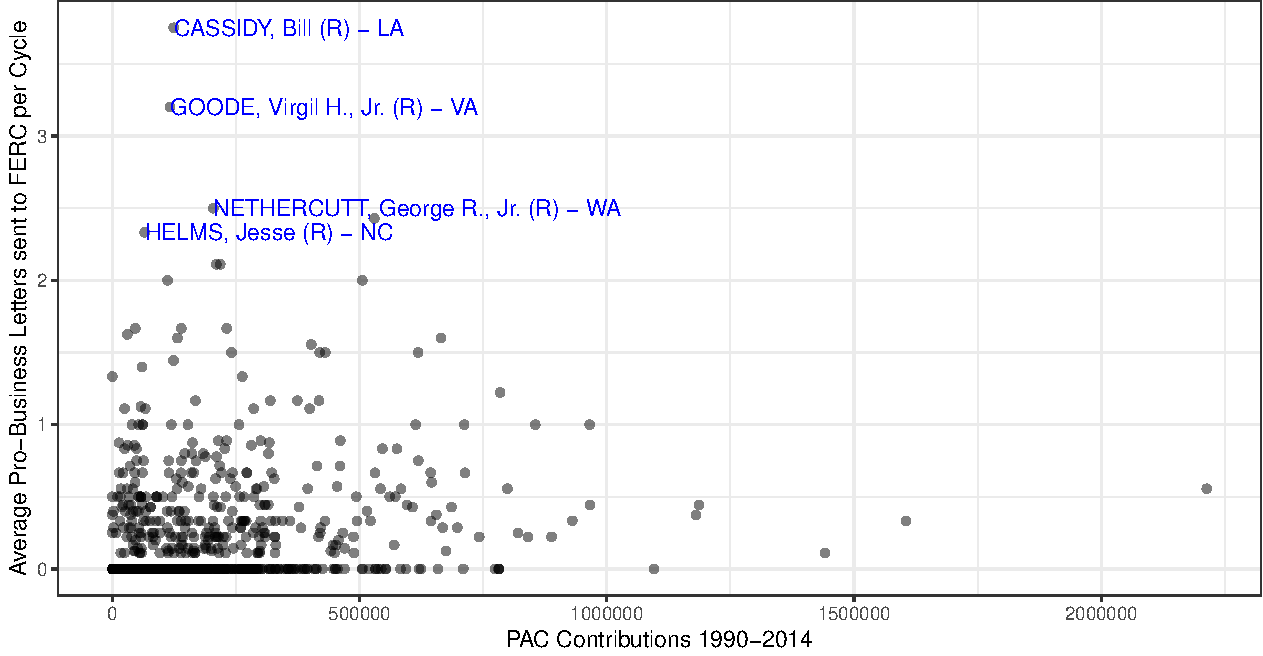
\includegraphics{Figs/letter_money-1} \end{center}

\begin{Shaded}
\begin{Highlighting}[]
\NormalTok{letters_money_total }\OperatorTok{%>%}\StringTok{ }
\StringTok{  }\KeywordTok{ggplot}\NormalTok{() }\OperatorTok{+}\StringTok{ }
\StringTok{  }\KeywordTok{coord_flip}\NormalTok{() }\OperatorTok{+}\StringTok{ }
\StringTok{  }\KeywordTok{aes}\NormalTok{(}\DataTypeTok{x =}\NormalTok{ PAC_contributions, }
      \DataTypeTok{y =}\NormalTok{ ProBusiness_Letters_Per_Cycle) }\OperatorTok{+}\StringTok{ }
\StringTok{  }\KeywordTok{geom_point}\NormalTok{(}\DataTypeTok{alpha =}\NormalTok{ .}\DecValTok{5}\NormalTok{) }\OperatorTok{+}\StringTok{ }
\StringTok{  }\KeywordTok{geom_text}\NormalTok{(}\KeywordTok{aes}\NormalTok{(}\DataTypeTok{label =} \KeywordTok{ifelse}\NormalTok{(name_state }\OperatorTok{%in%}\StringTok{ }\NormalTok{top1,}
\NormalTok{                               name_state, }\OtherTok{NA}\NormalTok{)), }\DataTypeTok{check_overlap =} \OtherTok{TRUE}\NormalTok{, }\DataTypeTok{hjust =} \DecValTok{0}\NormalTok{, }\DataTypeTok{color =} \StringTok{"blue"}\NormalTok{) }\OperatorTok{+}\StringTok{ }
\StringTok{  }
\StringTok{  }\KeywordTok{labs}\NormalTok{(}\DataTypeTok{x =} \StringTok{"PAC Contributions 1990-2014"}\NormalTok{,}
       \DataTypeTok{y =} \StringTok{"Average Pro-Business Letters sent to FERC per Cycle"}\NormalTok{)}
\end{Highlighting}
\end{Shaded}

\begin{center}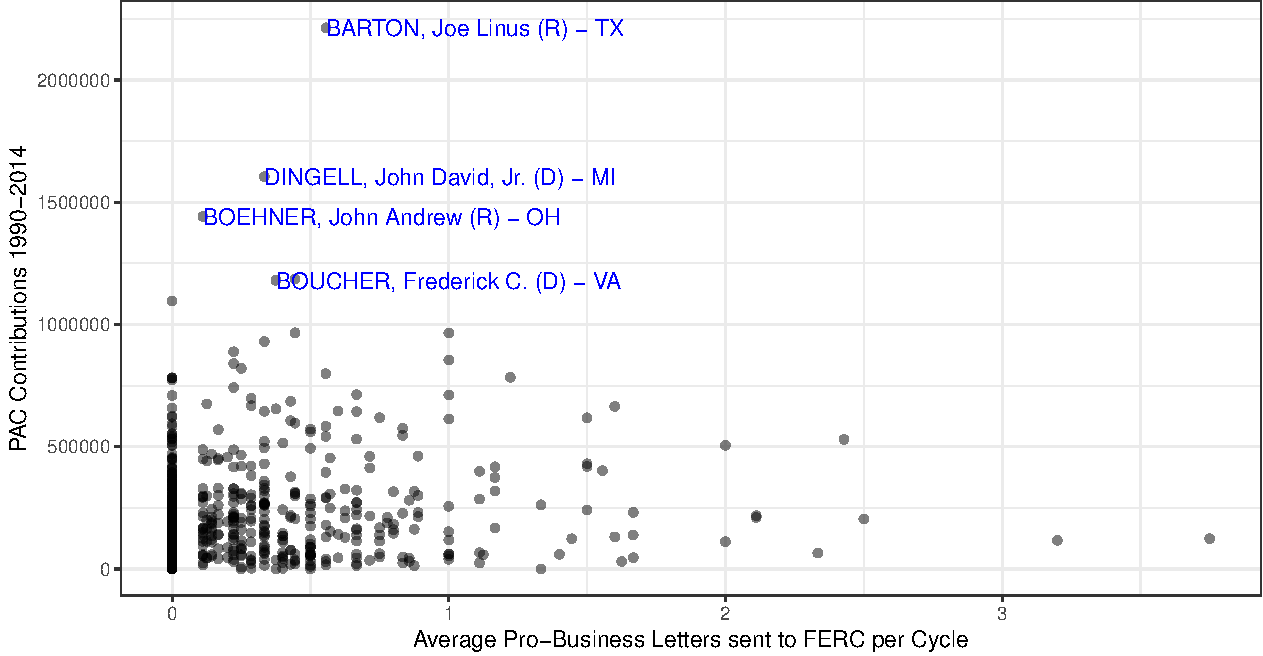
\includegraphics{Figs/letter_money-2} \end{center}

\section{Models}\label{models}

\subsection{Sector-level}\label{sector-level}

\subsubsection{All Letters per cycle \textasciitilde{} Energy Sector PAC
contributions per cycle
1998-2014}\label{all-letters-per-cycle-energy-sector-pac-contributions-per-cycle-1998-2014}

\begin{Shaded}
\begin{Highlighting}[]
\NormalTok{mplot <-}\StringTok{ }\ControlFlowTok{function}\NormalTok{(m)\{m }\OperatorTok{%>%}
\StringTok{  }\KeywordTok{tidy}\NormalTok{(}\DataTypeTok{conf.int =} \OtherTok{TRUE}\NormalTok{) }\OperatorTok{%>%}
\StringTok{    }\KeywordTok{filter}\NormalTok{(term}\OperatorTok{!=}\StringTok{"(Intercept)"}\NormalTok{) }\OperatorTok{%>%}
\KeywordTok{ggplot}\NormalTok{() }\OperatorTok{+}\StringTok{ }
\StringTok{  }\KeywordTok{aes}\NormalTok{(}\DataTypeTok{x =}\NormalTok{ term,}
      \DataTypeTok{y =}\NormalTok{ estimate, }
      \DataTypeTok{ymin =}\NormalTok{ conf.low, }
      \DataTypeTok{ymax =}\NormalTok{ conf.high)}\OperatorTok{+}\StringTok{ }
\StringTok{    }\KeywordTok{geom_hline}\NormalTok{(}\DataTypeTok{yintercept =} \DecValTok{0}\NormalTok{, }\DataTypeTok{linetype =}\DecValTok{2}\NormalTok{) }\OperatorTok{+}\StringTok{ }
\StringTok{  }\KeywordTok{geom_pointrange}\NormalTok{() }\OperatorTok{+}\StringTok{ }\KeywordTok{coord_flip}\NormalTok{() \}}

\NormalTok{All_Letters_money }\OperatorTok{%<>%}\StringTok{ }
\StringTok{  }\KeywordTok{mutate}\NormalTok{(}\DataTypeTok{Log_PAC_contributions =} \KeywordTok{log}\NormalTok{(PAC_contributions}\OperatorTok{+}\DecValTok{1}\NormalTok{))  }

\NormalTok{mAll <-}\StringTok{ }\KeywordTok{glm}\NormalTok{(All_Letters }\OperatorTok{~}\StringTok{ }\NormalTok{PAC_contributions, }\DataTypeTok{data =}\NormalTok{ All_Letters_money }\OperatorTok{%>%}
\StringTok{           }\KeywordTok{mutate}\NormalTok{(}\DataTypeTok{PAC_contributions =}\NormalTok{ PAC_contributions}\OperatorTok{/}\DecValTok{1000000}\NormalTok{), }
         \DataTypeTok{family =}\NormalTok{ poisson)  }
\KeywordTok{tidy}\NormalTok{(mAll)}
\end{Highlighting}
\end{Shaded}

\begin{verbatim}
## # A tibble: 2 x 5
##   term              estimate std.error statistic  p.value
##   <chr>                <dbl>     <dbl>     <dbl>    <dbl>
## 1 (Intercept)         -0.107    0.0164     -6.51 7.37e-11
## 2 PAC_contributions    3.11     0.267      11.6  2.70e-31
\end{verbatim}

\begin{Shaded}
\begin{Highlighting}[]
\NormalTok{mAll }\OperatorTok{%>%}\StringTok{ }\KeywordTok{mplot}\NormalTok{()}\OperatorTok{+}
\StringTok{  }\KeywordTok{labs}\NormalTok{(}\DataTypeTok{x=}\StringTok{""}\NormalTok{, }\DataTypeTok{y=}\StringTok{"Total additional letters per congress per million dollars"}\NormalTok{)}
\end{Highlighting}
\end{Shaded}

\begin{center}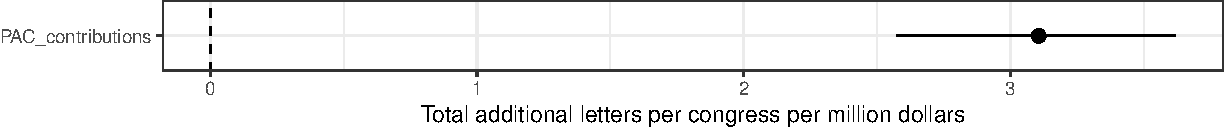
\includegraphics{Figs/all-letters-per-cycle-model-1} \end{center}

\paragraph{Pro-Business Letters per cycle \textasciitilde{} Energy
Sector PAC contributions per cycle
1998-2014}\label{pro-business-letters-per-cycle-energy-sector-pac-contributions-per-cycle-1998-2014}

\begin{Shaded}
\begin{Highlighting}[]
\NormalTok{letters_money }\OperatorTok{%<>%}\StringTok{ }
\StringTok{  }\KeywordTok{drop_na}\NormalTok{(ProBusiness_Letters, PAC_contributions) }\OperatorTok{%>%}
\StringTok{  }\KeywordTok{mutate}\NormalTok{(}\DataTypeTok{Log_PAC_contributions =} \KeywordTok{log}\NormalTok{(PAC_contributions}\OperatorTok{+}\DecValTok{1}\NormalTok{))  }

\NormalTok{mPro <-}\StringTok{ }\KeywordTok{glm}\NormalTok{(ProBusiness_Letters }\OperatorTok{~}\StringTok{ }\NormalTok{PAC_contributions, }\DataTypeTok{data =}\NormalTok{ letters_money }\OperatorTok{%>%}\StringTok{ }\KeywordTok{mutate}\NormalTok{(}\DataTypeTok{PAC_contributions =}\NormalTok{ PAC_contributions}\OperatorTok{/}\DecValTok{1000000}\NormalTok{), }\DataTypeTok{family =}\NormalTok{ poisson)  }
\KeywordTok{tidy}\NormalTok{(mPro)}
\end{Highlighting}
\end{Shaded}

\begin{verbatim}
## # A tibble: 2 x 5
##   term              estimate std.error statistic  p.value
##   <chr>                <dbl>     <dbl>     <dbl>    <dbl>
## 1 (Intercept)          -1.53    0.0340    -44.9  0       
## 2 PAC_contributions     2.24    0.600       3.74 0.000187
\end{verbatim}

\begin{Shaded}
\begin{Highlighting}[]
\NormalTok{mPro }\OperatorTok{%>%}\StringTok{ }\KeywordTok{mplot}\NormalTok{()}\OperatorTok{+}
\StringTok{  }\KeywordTok{labs}\NormalTok{(}\DataTypeTok{x=}\StringTok{""}\NormalTok{, }\DataTypeTok{y=}\StringTok{"Additional pro-business letters per congress per million dollars"}\NormalTok{)}
\end{Highlighting}
\end{Shaded}

\begin{center}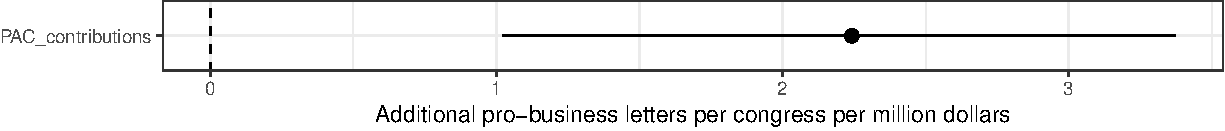
\includegraphics{Figs/money-letters-per-cycle-model-1} \end{center}

\begin{Shaded}
\begin{Highlighting}[]
\NormalTok{mProLog <-}\StringTok{ }\KeywordTok{glm}\NormalTok{(ProBusiness_Letters }\OperatorTok{~}\StringTok{ }\NormalTok{Log_PAC_contributions, }\DataTypeTok{data =}\NormalTok{ letters_money, }\DataTypeTok{family =}\NormalTok{ poisson  ) }
\KeywordTok{tidy}\NormalTok{(mProLog)}
\end{Highlighting}
\end{Shaded}

\begin{verbatim}
## # A tibble: 2 x 5
##   term                  estimate std.error statistic   p.value
##   <chr>                    <dbl>     <dbl>     <dbl>     <dbl>
## 1 (Intercept)           -1.53      0.0656     -23.3  6.66e-120
## 2 Log_PAC_contributions  0.00786   0.00741      1.06 2.89e-  1
\end{verbatim}

\begin{Shaded}
\begin{Highlighting}[]
\NormalTok{mProLog }\OperatorTok{%>%}\StringTok{ }\KeywordTok{mplot}\NormalTok{()}\OperatorTok{+}
\StringTok{  }\KeywordTok{labs}\NormalTok{(}\DataTypeTok{x=}\StringTok{""}\NormalTok{, }\DataTypeTok{y=}\StringTok{"Additional letters per congress per Log(PAC Contributions)"}\NormalTok{)}
\end{Highlighting}
\end{Shaded}

\begin{center}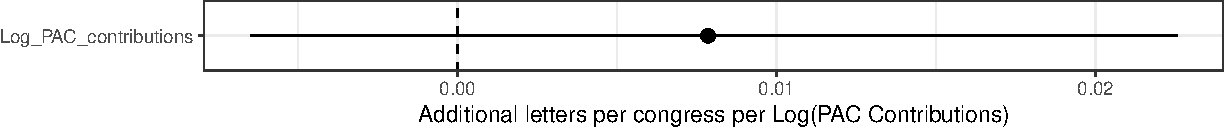
\includegraphics{Figs/money-letters-per-cycle-model-2} \end{center}

\begin{Shaded}
\begin{Highlighting}[]
\NormalTok{mNonConstituent <-}\StringTok{ }\KeywordTok{glm}\NormalTok{(Non_Constituent_Letters }\OperatorTok{~}\StringTok{ }\NormalTok{PAC_contributions, }\DataTypeTok{data =}\NormalTok{ Non_Constituent_money, }\DataTypeTok{family =}\NormalTok{ poisson  ) }
\KeywordTok{tidy}\NormalTok{(mNonConstituent)}
\end{Highlighting}
\end{Shaded}

\begin{verbatim}
## # A tibble: 2 x 5
##   term                 estimate   std.error statistic  p.value
##   <chr>                   <dbl>       <dbl>     <dbl>    <dbl>
## 1 (Intercept)       -0.107      0.0164          -6.51 7.37e-11
## 2 PAC_contributions  0.00000311 0.000000267     11.6  2.70e-31
\end{verbatim}

\begin{Shaded}
\begin{Highlighting}[]
\NormalTok{mNonConstituent }\OperatorTok{%>%}\StringTok{ }\KeywordTok{mplot}\NormalTok{()}\OperatorTok{+}
\StringTok{  }\KeywordTok{labs}\NormalTok{(}\DataTypeTok{x=}\StringTok{""}\NormalTok{, }\DataTypeTok{y=}\StringTok{"Additional non-constituent letters per congress per million dollars"}\NormalTok{)}
\end{Highlighting}
\end{Shaded}

\begin{center}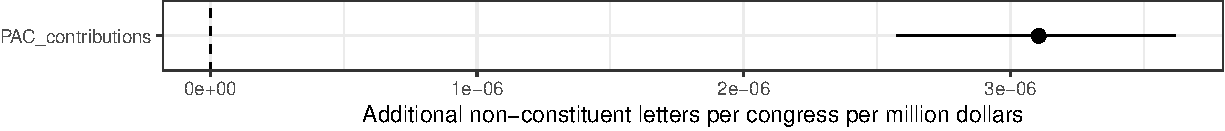
\includegraphics{Figs/money-letters-per-cycle-model-3} \end{center}

By party:

\begin{Shaded}
\begin{Highlighting}[]
\NormalTok{mProParty <-}\StringTok{ }\KeywordTok{glm}\NormalTok{(ProBusiness_Letters }\OperatorTok{~}\StringTok{ }\NormalTok{party, }\DataTypeTok{data =}\NormalTok{ letters_money }\OperatorTok{%>%}\StringTok{ }\KeywordTok{filter}\NormalTok{(party }\OperatorTok{!=}\StringTok{"NA"}\NormalTok{), }\DataTypeTok{family =} \StringTok{"poisson"}\NormalTok{ ) }

\KeywordTok{tidy}\NormalTok{(mProParty)}
\end{Highlighting}
\end{Shaded}

\begin{verbatim}
## # A tibble: 2 x 5
##   term        estimate std.error statistic   p.value
##   <chr>          <dbl>     <dbl>     <dbl>     <dbl>
## 1 (Intercept)   -1.24     0.0425    -29.1  1.26e-186
## 2 party(R)       0.206    0.0580      3.56 3.75e-  4
\end{verbatim}

\begin{Shaded}
\begin{Highlighting}[]
\KeywordTok{mplot}\NormalTok{(mProParty) }\OperatorTok{+}
\StringTok{  }\KeywordTok{labs}\NormalTok{(}\DataTypeTok{x=}\StringTok{""}\NormalTok{, }\DataTypeTok{y=}\StringTok{"Additional letters per congress"}\NormalTok{)}
\end{Highlighting}
\end{Shaded}

\begin{center}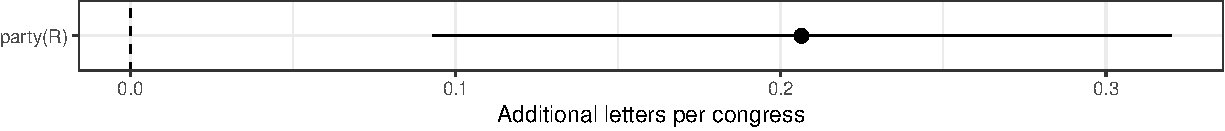
\includegraphics{Figs/letters-per-cycle-model-party-1} \end{center}

Republicans send an additional 0.2 letters per Congress, on average.

\begin{Shaded}
\begin{Highlighting}[]
\CommentTok{# PAC + party:}
\NormalTok{mPro_pac_party<-}\KeywordTok{glm}\NormalTok{(ProBusiness_Letters }\OperatorTok{~}\StringTok{ }\NormalTok{PAC_contributions }\OperatorTok{+}\StringTok{ }\NormalTok{party, }\DataTypeTok{data =}\NormalTok{ letters_money }\OperatorTok{%>%}\StringTok{ }\KeywordTok{filter}\NormalTok{(party }\OperatorTok{!=}\StringTok{"NA"}\NormalTok{)}\OperatorTok{%>%}\StringTok{ }\KeywordTok{mutate}\NormalTok{(}\DataTypeTok{PAC_contributions =}\NormalTok{ PAC_contributions}\OperatorTok{/}\DecValTok{1000000}\NormalTok{), }\DataTypeTok{family =} \StringTok{"poisson"}\NormalTok{ )  }
\KeywordTok{tidy}\NormalTok{(mPro_pac_party)}
\end{Highlighting}
\end{Shaded}

\begin{verbatim}
## # A tibble: 3 x 5
##   term              estimate std.error statistic   p.value
##   <chr>                <dbl>     <dbl>     <dbl>     <dbl>
## 1 (Intercept)         -1.25     0.0444   -28.1   7.04e-174
## 2 PAC_contributions    0.452    0.641      0.705 4.81e-  1
## 3 party(R)             0.198    0.0592     3.34  8.24e-  4
\end{verbatim}

\begin{Shaded}
\begin{Highlighting}[]
\KeywordTok{mplot}\NormalTok{(mPro_pac_party)}\OperatorTok{+}
\StringTok{  }\KeywordTok{labs}\NormalTok{(}\DataTypeTok{x=}\StringTok{""}\NormalTok{, }\DataTypeTok{y=}\StringTok{"Additional letters per congress"}\NormalTok{)}
\end{Highlighting}
\end{Shaded}

\begin{center}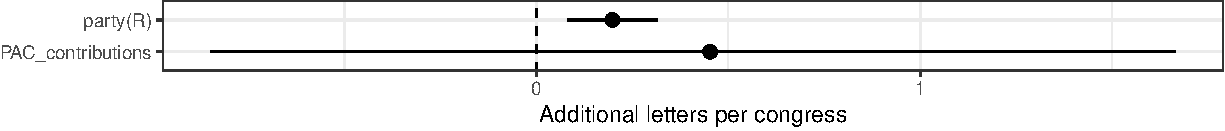
\includegraphics{Figs/multivariate_model-1} \end{center}

\begin{Shaded}
\begin{Highlighting}[]
\CommentTok{# PAC*party interaction:}
\NormalTok{mPro_pacXparty<-}\KeywordTok{glm}\NormalTok{(ProBusiness_Letters }\OperatorTok{~}\StringTok{ }\NormalTok{PAC_contributions }\OperatorTok{*}\StringTok{ }\NormalTok{party, }\DataTypeTok{data =}\NormalTok{ letters_money }\OperatorTok{%>%}\StringTok{ }\KeywordTok{filter}\NormalTok{(party }\OperatorTok{!=}\StringTok{"NA"}\NormalTok{)}\OperatorTok{%>%}\StringTok{ }\KeywordTok{mutate}\NormalTok{(}\DataTypeTok{PAC_contributions =}\NormalTok{ PAC_contributions}\OperatorTok{/}\DecValTok{1000000}\NormalTok{), }\DataTypeTok{family =} \StringTok{"poisson"}\NormalTok{ )  }
\KeywordTok{tidy}\NormalTok{(mPro_pacXparty)}
\end{Highlighting}
\end{Shaded}

\begin{verbatim}
## # A tibble: 4 x 5
##   term                       estimate std.error statistic   p.value
##   <chr>                         <dbl>     <dbl>     <dbl>     <dbl>
## 1 (Intercept)                  -1.26     0.0492   -25.6   3.19e-144
## 2 PAC_contributions             0.963    1.21       0.796 4.26e-  1
## 3 party(R)                      0.216    0.0693     3.11  1.87e-  3
## 4 PAC_contributions:party(R)   -0.702    1.43      -0.491 6.23e-  1
\end{verbatim}

\begin{Shaded}
\begin{Highlighting}[]
\KeywordTok{mplot}\NormalTok{(mPro_pacXparty)}\OperatorTok{+}
\StringTok{  }\KeywordTok{labs}\NormalTok{(}\DataTypeTok{x=}\StringTok{""}\NormalTok{, }\DataTypeTok{y=}\StringTok{"Additional letters per congress"}\NormalTok{)}
\end{Highlighting}
\end{Shaded}

\begin{center}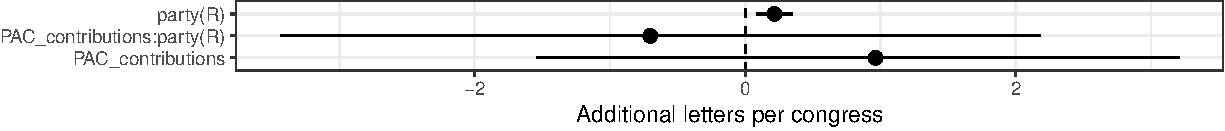
\includegraphics{Figs/multivariate_model-2} \end{center}

\begin{Shaded}
\begin{Highlighting}[]
\NormalTok{letters_money }\OperatorTok{%<>%}\StringTok{ }\KeywordTok{left_join}\NormalTok{(d }\OperatorTok{%>%}\StringTok{ }\KeywordTok{select}\NormalTok{(icpsryear, nominate.dim1, chair_since_}\DecValTok{2007}\NormalTok{, oversight_committee)) }\OperatorTok{%>%}\StringTok{ }\KeywordTok{rename}\NormalTok{(}\DataTypeTok{chair =}\NormalTok{ chair_since_}\DecValTok{2007}\NormalTok{)}

\CommentTok{# DW NOMINATE }
\NormalTok{mPro_nominate <-}\KeywordTok{glm}\NormalTok{(ProBusiness_Letters }\OperatorTok{~}\StringTok{  }\NormalTok{nominate.dim1, }\DataTypeTok{data =}\NormalTok{ letters_money }\OperatorTok{%>%}\StringTok{ }\KeywordTok{filter}\NormalTok{(party }\OperatorTok{!=}\StringTok{"NA"}\NormalTok{)}\OperatorTok{%>%}\StringTok{ }\KeywordTok{mutate}\NormalTok{(}\DataTypeTok{PAC_contributions =}\NormalTok{ PAC_contributions}\OperatorTok{/}\DecValTok{1000000}\NormalTok{), }\DataTypeTok{family =} \StringTok{"poisson"}\NormalTok{ )  }
\KeywordTok{tidy}\NormalTok{(mPro_nominate)}
\end{Highlighting}
\end{Shaded}

\begin{verbatim}
## # A tibble: 2 x 5
##   term          estimate std.error statistic   p.value
##   <chr>            <dbl>     <dbl>     <dbl>     <dbl>
## 1 (Intercept)      0.326    0.0120      27.2 1.93e-163
## 2 nominate.dim1    0.404    0.0303      13.3 1.37e- 40
\end{verbatim}

\begin{Shaded}
\begin{Highlighting}[]
\KeywordTok{mplot}\NormalTok{(mPro_nominate)}\OperatorTok{+}
\StringTok{  }\KeywordTok{labs}\NormalTok{(}\DataTypeTok{x=}\StringTok{""}\NormalTok{, }\DataTypeTok{y=}\StringTok{"Additional letters per congress"}\NormalTok{)}
\end{Highlighting}
\end{Shaded}

\begin{center}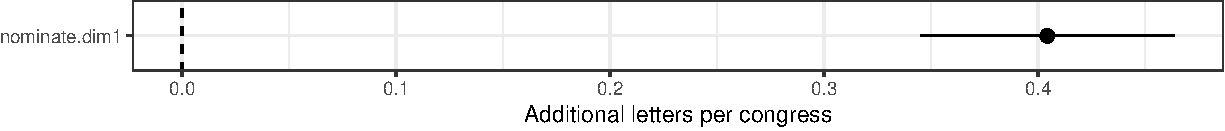
\includegraphics{Figs/multivariate_model-3} \end{center}

\begin{Shaded}
\begin{Highlighting}[]
\CommentTok{# PAC + ideology:}
\NormalTok{mPro_pac_nominate <-}\KeywordTok{glm}\NormalTok{(ProBusiness_Letters }\OperatorTok{~}\StringTok{ }\NormalTok{PAC_contributions }\OperatorTok{*}\StringTok{ }\NormalTok{nominate.dim1, }\DataTypeTok{data =}\NormalTok{ letters_money }\OperatorTok{%>%}\StringTok{ }\KeywordTok{filter}\NormalTok{(party }\OperatorTok{!=}\StringTok{"NA"}\NormalTok{)}\OperatorTok{%>%}\StringTok{ }\KeywordTok{mutate}\NormalTok{(}\DataTypeTok{PAC_contributions =}\NormalTok{ PAC_contributions}\OperatorTok{/}\DecValTok{1000000}\NormalTok{), }\DataTypeTok{family =} \StringTok{"poisson"}\NormalTok{ )  }
\KeywordTok{tidy}\NormalTok{(mPro_pac_nominate)}
\end{Highlighting}
\end{Shaded}

\begin{verbatim}
## # A tibble: 4 x 5
##   term                            estimate std.error statistic   p.value
##   <chr>                              <dbl>     <dbl>     <dbl>     <dbl>
## 1 (Intercept)                        0.426    0.0142     30.1  1.43e-198
## 2 PAC_contributions                 -3.30     0.325     -10.1  4.08e- 24
## 3 nominate.dim1                      0.522    0.0356     14.6  1.51e- 48
## 4 PAC_contributions:nominate.dim1   -1.28     0.834      -1.53 1.26e-  1
\end{verbatim}

\begin{Shaded}
\begin{Highlighting}[]
\KeywordTok{mplot}\NormalTok{(mPro_pac_nominate)}\OperatorTok{+}
\StringTok{  }\KeywordTok{labs}\NormalTok{(}\DataTypeTok{x=}\StringTok{""}\NormalTok{, }\DataTypeTok{y=}\StringTok{"Additional letters per congress"}\NormalTok{)}
\end{Highlighting}
\end{Shaded}

\begin{center}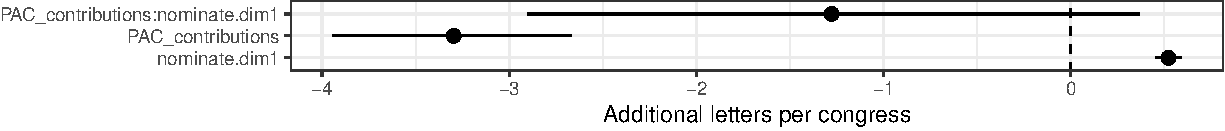
\includegraphics{Figs/multivariate_model-4} \end{center}

\begin{Shaded}
\begin{Highlighting}[]
\CommentTok{# Full model:}
\NormalTok{mPro_Full <-}\StringTok{ }\KeywordTok{glm}\NormalTok{(ProBusiness_Letters }\OperatorTok{~}\StringTok{ }\NormalTok{PAC_contributions }\OperatorTok{+}\StringTok{ }\NormalTok{nominate.dim1 }\OperatorTok{+}\StringTok{ }\NormalTok{chair, oversight_committee, }\DataTypeTok{data =}\NormalTok{ letters_money }\OperatorTok{%>%}\StringTok{ }\KeywordTok{filter}\NormalTok{(party }\OperatorTok{!=}\StringTok{"NA"}\NormalTok{)}\OperatorTok{%>%}\StringTok{ }\KeywordTok{mutate}\NormalTok{(}\DataTypeTok{PAC_contributions =}\NormalTok{ PAC_contributions}\OperatorTok{/}\DecValTok{1000000}\NormalTok{), }\DataTypeTok{family =} \StringTok{"poisson"}\NormalTok{ )  }
\KeywordTok{tidy}\NormalTok{(mPro_Full)}
\end{Highlighting}
\end{Shaded}

\begin{verbatim}
## # A tibble: 4 x 5
##   term              estimate std.error statistic  p.value
##   <chr>                <dbl>     <dbl>     <dbl>    <dbl>
## 1 (Intercept)          0.193    0.0259      7.45 9.15e-14
## 2 PAC_contributions   -3.18     0.344      -9.24 2.47e-20
## 3 nominate.dim1        0.549    0.0457     12.0  3.11e-33
## 4 chairTRUE            0.490    0.0336     14.6  4.47e-48
\end{verbatim}

\begin{Shaded}
\begin{Highlighting}[]
\KeywordTok{mplot}\NormalTok{(mPro_Full)}\OperatorTok{+}
\StringTok{  }\KeywordTok{labs}\NormalTok{(}\DataTypeTok{x=}\StringTok{""}\NormalTok{, }\DataTypeTok{y=}\StringTok{"Additional letters per congress"}\NormalTok{)}
\end{Highlighting}
\end{Shaded}

\begin{center}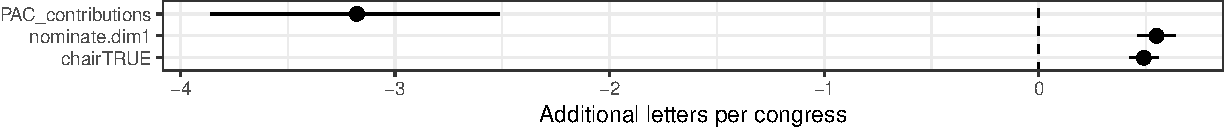
\includegraphics{Figs/multivariate_model-5} \end{center}

\paragraph{Average Pro-Business letters per cycle \textasciitilde{}
total Energy Sector PAC contributions
1990-2014}\label{average-pro-business-letters-per-cycle-total-energy-sector-pac-contributions-1990-2014}

\begin{Shaded}
\begin{Highlighting}[]
\NormalTok{mProTotal <-}\StringTok{ }\KeywordTok{glm}\NormalTok{(ProBusiness_Letters_Per_Cycle }\OperatorTok{~}\StringTok{ }\NormalTok{PAC_contributions, }\DataTypeTok{data =}\NormalTok{ letters_money_total}\OperatorTok{%>%}\StringTok{ }\KeywordTok{mutate}\NormalTok{(}\DataTypeTok{PAC_contributions =}\NormalTok{ PAC_contributions}\OperatorTok{/}\DecValTok{1000000}\NormalTok{), }\DataTypeTok{family =} \StringTok{"poisson"}\NormalTok{)  }

\KeywordTok{tidy}\NormalTok{(mProTotal)}
\end{Highlighting}
\end{Shaded}

\begin{verbatim}
## # A tibble: 2 x 5
##   term              estimate std.error statistic  p.value
##   <chr>                <dbl>     <dbl>     <dbl>    <dbl>
## 1 (Intercept)          -1.87    0.0941    -19.8  1.51e-87
## 2 PAC_contributions     1.19    0.221       5.39 7.03e- 8
\end{verbatim}

\begin{Shaded}
\begin{Highlighting}[]
\KeywordTok{mplot}\NormalTok{(mProTotal)}\OperatorTok{+}
\StringTok{  }\KeywordTok{labs}\NormalTok{(}\DataTypeTok{x=}\StringTok{""}\NormalTok{, }\DataTypeTok{y=}\StringTok{"Average additional letters per cycle per million dollars 1990-2014"}\NormalTok{)}
\end{Highlighting}
\end{Shaded}

\begin{center}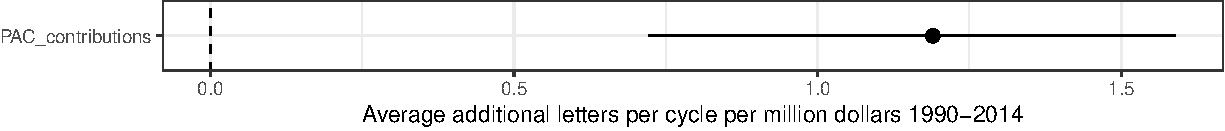
\includegraphics{Figs/money-letters-total-1} \end{center}

\paragraph{Anti-Business Letters per cycle \textasciitilde{} Energy
Sector PAC contributions per cycle
1998-2014}\label{anti-business-letters-per-cycle-energy-sector-pac-contributions-per-cycle-1998-2014}

\begin{Shaded}
\begin{Highlighting}[]
\NormalTok{Antiletters_money }\OperatorTok{%<>%}\StringTok{ }
\StringTok{  }\KeywordTok{drop_na}\NormalTok{(AntiBusiness_Letters, PAC_contributions) }\OperatorTok{%>%}\StringTok{ }\KeywordTok{mutate}\NormalTok{(}\DataTypeTok{Log_PAC_contributions =} \KeywordTok{log}\NormalTok{(PAC_contributions}\OperatorTok{+}\DecValTok{1}\NormalTok{)) }

\NormalTok{mAnti <-}\StringTok{ }\KeywordTok{glm}\NormalTok{(AntiBusiness_Letters }\OperatorTok{~}\StringTok{ }\NormalTok{PAC_contributions, }\DataTypeTok{data =}\NormalTok{ Antiletters_money }\OperatorTok{%>%}\StringTok{ }\KeywordTok{mutate}\NormalTok{(}\DataTypeTok{PAC_contributions =}\NormalTok{ PAC_contributions}\OperatorTok{/}\DecValTok{1000000}\NormalTok{), }\DataTypeTok{family =}\NormalTok{ poisson)  }
\KeywordTok{tidy}\NormalTok{(mAnti)}
\end{Highlighting}
\end{Shaded}

\begin{verbatim}
## # A tibble: 2 x 5
##   term              estimate std.error statistic   p.value
##   <chr>                <dbl>     <dbl>     <dbl>     <dbl>
## 1 (Intercept)         -0.977    0.0267   -36.6   1.31e-292
## 2 PAC_contributions    0.476    0.546      0.872 3.83e-  1
\end{verbatim}

\begin{Shaded}
\begin{Highlighting}[]
\NormalTok{mAnti }\OperatorTok{%>%}\StringTok{ }\KeywordTok{mplot}\NormalTok{()}\OperatorTok{+}
\StringTok{  }\KeywordTok{labs}\NormalTok{(}\DataTypeTok{x=}\StringTok{""}\NormalTok{, }\DataTypeTok{y=}\StringTok{"Additional anti-buisness letters per congress per million dollars"}\NormalTok{)}
\end{Highlighting}
\end{Shaded}

\begin{center}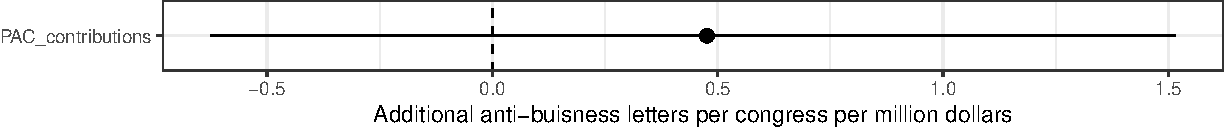
\includegraphics{Figs/money-Antiletters-per-cycle-model-1} \end{center}

\begin{Shaded}
\begin{Highlighting}[]
\NormalTok{mAntiLog <-}\StringTok{ }\KeywordTok{glm}\NormalTok{(AntiBusiness_Letters }\OperatorTok{~}\StringTok{ }\NormalTok{Log_PAC_contributions, }\DataTypeTok{data =}\NormalTok{ Antiletters_money, }\DataTypeTok{family =}\NormalTok{ poisson  ) }
\KeywordTok{tidy}\NormalTok{(mAntiLog)}
\end{Highlighting}
\end{Shaded}

\begin{verbatim}
## # A tibble: 2 x 5
##   term                  estimate std.error statistic  p.value
##   <chr>                    <dbl>     <dbl>     <dbl>    <dbl>
## 1 (Intercept)            -0.840    0.0468     -17.9  6.09e-72
## 2 Log_PAC_contributions  -0.0162   0.00544     -2.98 2.88e- 3
\end{verbatim}

\begin{Shaded}
\begin{Highlighting}[]
\NormalTok{mAntiLog }\OperatorTok{%>%}\StringTok{ }\KeywordTok{mplot}\NormalTok{()}\OperatorTok{+}
\StringTok{  }\KeywordTok{labs}\NormalTok{(}\DataTypeTok{x=}\StringTok{""}\NormalTok{, }\DataTypeTok{y=}\StringTok{"Additional anti-business Letters per congress per Log(PAC Contributions)"}\NormalTok{)}
\end{Highlighting}
\end{Shaded}

\begin{center}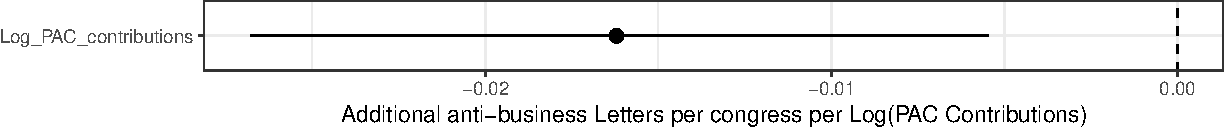
\includegraphics{Figs/money-Antiletters-per-cycle-model-2} \end{center}

By party:

\begin{Shaded}
\begin{Highlighting}[]
\NormalTok{mAntiParty <-}\StringTok{ }\KeywordTok{glm}\NormalTok{(AntiBusiness_Letters }\OperatorTok{~}\StringTok{ }\NormalTok{party, }\DataTypeTok{data =}\NormalTok{ Antiletters_money }\OperatorTok{%>%}\StringTok{ }\KeywordTok{filter}\NormalTok{(party }\OperatorTok{!=}\StringTok{"NA"}\NormalTok{), }\DataTypeTok{family =} \StringTok{"poisson"}\NormalTok{ ) }

\KeywordTok{tidy}\NormalTok{(mAntiParty)}
\end{Highlighting}
\end{Shaded}

\begin{verbatim}
## # A tibble: 2 x 5
##   term        estimate std.error statistic  p.value
##   <chr>          <dbl>     <dbl>     <dbl>    <dbl>
## 1 (Intercept)   -0.479    0.0291    -16.5  4.98e-61
## 2 party(R)      -0.348    0.0460     -7.57 3.60e-14
\end{verbatim}

\begin{Shaded}
\begin{Highlighting}[]
\KeywordTok{mplot}\NormalTok{(mAntiParty) }\OperatorTok{+}
\StringTok{  }\KeywordTok{labs}\NormalTok{(}\DataTypeTok{x=}\StringTok{""}\NormalTok{, }\DataTypeTok{y=}\StringTok{"Additional anti-business  letters per congress"}\NormalTok{)}
\end{Highlighting}
\end{Shaded}

\begin{center}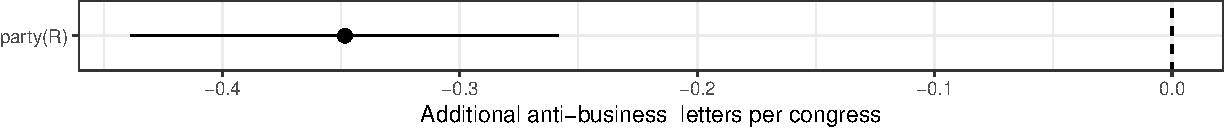
\includegraphics{Figs/Antiletters-per-cycle-model-party-1} \end{center}

Democrats send an additional 0.3 Anti-Business letters per Congress, on
average.

\begin{Shaded}
\begin{Highlighting}[]
\CommentTok{#PAC*party interaction:}
\NormalTok{mAnti_pacXparty <-}\KeywordTok{glm}\NormalTok{(AntiBusiness_Letters }\OperatorTok{~}\StringTok{ }\NormalTok{PAC_contributions}\OperatorTok{*}\NormalTok{party, }\DataTypeTok{data =}\NormalTok{ Antiletters_money }\OperatorTok{%>%}\StringTok{ }\KeywordTok{filter}\NormalTok{(party }\OperatorTok{!=}\StringTok{"NA"}\NormalTok{)}\OperatorTok{%>%}\StringTok{ }\KeywordTok{mutate}\NormalTok{(}\DataTypeTok{PAC_contributions =}\NormalTok{ PAC_contributions}\OperatorTok{/}\DecValTok{1000000}\NormalTok{), }\DataTypeTok{family =} \StringTok{"poisson"}\NormalTok{ )  }
\KeywordTok{tidy}\NormalTok{(mAnti_pacXparty)}
\end{Highlighting}
\end{Shaded}

\begin{verbatim}
## # A tibble: 4 x 5
##   term                       estimate std.error statistic  p.value
##   <chr>                         <dbl>     <dbl>     <dbl>    <dbl>
## 1 (Intercept)                  -0.493    0.0337   -14.6   1.82e-48
## 2 PAC_contributions             0.674    0.844      0.798 4.25e- 1
## 3 party(R)                     -0.312    0.0557    -5.60  2.12e- 8
## 4 PAC_contributions:party(R)   -1.31     1.12      -1.17  2.43e- 1
\end{verbatim}

\begin{Shaded}
\begin{Highlighting}[]
\KeywordTok{mplot}\NormalTok{(mAnti_pacXparty)}\OperatorTok{+}
\StringTok{  }\KeywordTok{labs}\NormalTok{(}\DataTypeTok{x=}\StringTok{""}\NormalTok{, }\DataTypeTok{y=}\StringTok{"Additional anti-business letters per congress"}\NormalTok{)}
\end{Highlighting}
\end{Shaded}

\begin{center}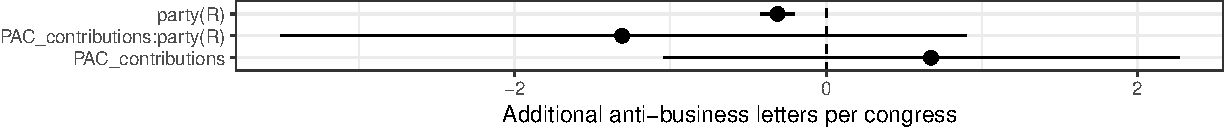
\includegraphics{Figs/money-Antiletters-per-cycle-model-party-1} \end{center}

\paragraph{Average Anti-Business letters per cycle \textasciitilde{}
total Energy Sector PAC contributions
1990-2014}\label{average-anti-business-letters-per-cycle-total-energy-sector-pac-contributions-1990-2014}

\begin{Shaded}
\begin{Highlighting}[]
\NormalTok{mAntiTotal <-}\StringTok{ }\KeywordTok{glm}\NormalTok{(AntiBusiness_Letters_Per_Cycle }\OperatorTok{~}\StringTok{ }\NormalTok{PAC_contributions, }\DataTypeTok{data =}\NormalTok{ Antiletters_money_total}\OperatorTok{%>%}\StringTok{ }\KeywordTok{mutate}\NormalTok{(}\DataTypeTok{PAC_contributions =}\NormalTok{ PAC_contributions}\OperatorTok{/}\DecValTok{1000000}\NormalTok{), }\DataTypeTok{family =} \StringTok{"poisson"}\NormalTok{)  }

\KeywordTok{tidy}\NormalTok{(mAntiTotal)}
\end{Highlighting}
\end{Shaded}

\begin{verbatim}
## # A tibble: 2 x 5
##   term              estimate std.error statistic  p.value
##   <chr>                <dbl>     <dbl>     <dbl>    <dbl>
## 1 (Intercept)         -1.27     0.0768    -16.5  2.62e-61
## 2 PAC_contributions    0.628    0.231       2.72 6.54e- 3
\end{verbatim}

\begin{Shaded}
\begin{Highlighting}[]
\KeywordTok{mplot}\NormalTok{(mAntiTotal)}\OperatorTok{+}
\StringTok{  }\KeywordTok{labs}\NormalTok{(}\DataTypeTok{x=}\StringTok{""}\NormalTok{, }\DataTypeTok{y=}\StringTok{"Average additional anti-business letters per cycle per million dollars 1990-2014"}\NormalTok{)}
\end{Highlighting}
\end{Shaded}

\begin{center}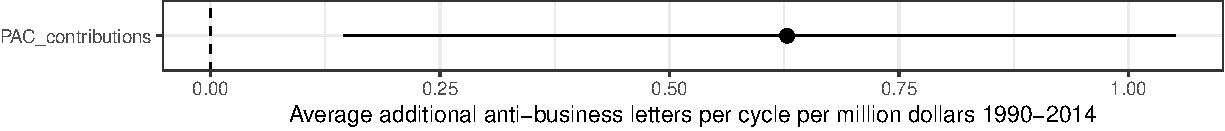
\includegraphics{Figs/money-Antiletters-total-1} \end{center}

\begin{Shaded}
\begin{Highlighting}[]
\NormalTok{dplot <-}\StringTok{ }\ControlFlowTok{function}\NormalTok{(x)\{}\KeywordTok{dwplot}\NormalTok{(x) }\OperatorTok{+}
\StringTok{    }\KeywordTok{aes}\NormalTok{(}\DataTypeTok{shape =}\NormalTok{ model) }\OperatorTok{+}\StringTok{ }
\StringTok{    }\KeywordTok{geom_vline}\NormalTok{(}\DataTypeTok{xintercept =} \DecValTok{0}\NormalTok{, }\DataTypeTok{linetype =} \DecValTok{2}\NormalTok{) }\OperatorTok{+}
\StringTok{    }\KeywordTok{scale_color_viridis_d}\NormalTok{(}\DataTypeTok{option =} \StringTok{"C"}\NormalTok{, }\DataTypeTok{end =}\NormalTok{ .}\DecValTok{8}\NormalTok{) }\OperatorTok{+}\StringTok{ }
\StringTok{    }\KeywordTok{labs}\NormalTok{(}\DataTypeTok{color =} \StringTok{"Dependent Variable"}\NormalTok{,}
         \DataTypeTok{shape =} \StringTok{"Dependent Variable"}\NormalTok{) }\OperatorTok{+}
\StringTok{  }\KeywordTok{theme}\NormalTok{(}\DataTypeTok{panel.grid.major.y  =} \KeywordTok{element_blank}\NormalTok{())}
\NormalTok{\}}

\CommentTok{# Basic PAC money models }
\NormalTok{models <-}\StringTok{ }\KeywordTok{full_join}\NormalTok{(}
  \KeywordTok{tidy}\NormalTok{(mAll) }\OperatorTok{%>%}\StringTok{ }\KeywordTok{mutate}\NormalTok{(}\DataTypeTok{model =} \StringTok{"All Letters per Cycle"}\NormalTok{),}
  \KeywordTok{tidy}\NormalTok{(mPro) }\OperatorTok{%>%}\StringTok{ }\KeywordTok{mutate}\NormalTok{(}\DataTypeTok{model =} \StringTok{"Pro-business Letters per Cycle"}\NormalTok{) ) }\OperatorTok{%>%}\StringTok{ }
\StringTok{  }\KeywordTok{full_join}\NormalTok{(}\KeywordTok{tidy}\NormalTok{(mNonConstituent) }\OperatorTok{%>%}\StringTok{ }\KeywordTok{mutate}\NormalTok{(}\DataTypeTok{model =} \StringTok{"Non-constituent Letters per Cycle"}\NormalTok{)) }\OperatorTok{%>%}
\StringTok{  }\KeywordTok{full_join}\NormalTok{(}\KeywordTok{tidy}\NormalTok{(mAnti)  }\OperatorTok{%>%}\StringTok{ }\KeywordTok{mutate}\NormalTok{(}\DataTypeTok{model =} \StringTok{"Anti-business Letters per Cycle"}\NormalTok{)) }

\KeywordTok{dplot}\NormalTok{(models)}\OperatorTok{+}\StringTok{ }
\StringTok{    }\KeywordTok{labs}\NormalTok{(}\DataTypeTok{color =} \StringTok{"Dependent Variable"}\NormalTok{,}
         \DataTypeTok{shape =} \StringTok{"Dependent Variable"}\NormalTok{,}
         \DataTypeTok{x =} \StringTok{"Additional letters per million dollars per cycle"}\NormalTok{)}
\end{Highlighting}
\end{Shaded}

\begin{center}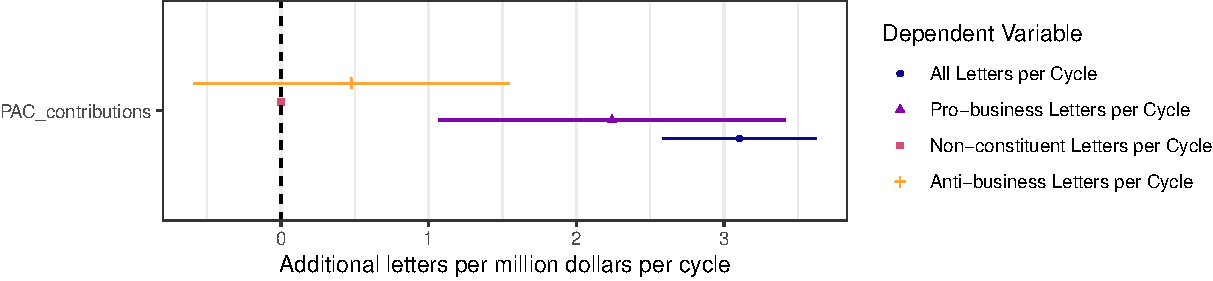
\includegraphics{Figs/models-1} \end{center}

\begin{Shaded}
\begin{Highlighting}[]
\NormalTok{knitr}\OperatorTok{::}\KeywordTok{kable}\NormalTok{(models }\OperatorTok{%>%}\StringTok{ }\NormalTok{dplyr}\OperatorTok{::}\KeywordTok{select}\NormalTok{(model, }\KeywordTok{everything}\NormalTok{()), }\DataTypeTok{digets =} \DecValTok{3}\NormalTok{, }\DataTypeTok{caption =} \StringTok{"Additional letters per million dollars per cycle"}\NormalTok{)}
\end{Highlighting}
\end{Shaded}

\begin{longtable}[]{@{}llrrrr@{}}
\caption{Additional letters per million dollars per
cycle}\tabularnewline
\toprule
model & term & estimate & std.error & statistic & p.value\tabularnewline
\midrule
\endfirsthead
\toprule
model & term & estimate & std.error & statistic & p.value\tabularnewline
\midrule
\endhead
All Letters per Cycle & (Intercept) & -0.1070478 & 0.0164362 &
-6.5129251 & 0.0000000\tabularnewline
All Letters per Cycle & PAC\_contributions & 3.1061544 & 0.2669378 &
11.6362471 & 0.0000000\tabularnewline
Pro-business Letters per Cycle & (Intercept) & -1.5265255 & 0.0340234 &
-44.8669425 & 0.0000000\tabularnewline
Pro-business Letters per Cycle & PAC\_contributions & 2.2422052 &
0.6001300 & 3.7361989 & 0.0001868\tabularnewline
Non-constituent Letters per Cycle & (Intercept) & -0.1070478 & 0.0164362
& -6.5129251 & 0.0000000\tabularnewline
Non-constituent Letters per Cycle & PAC\_contributions & 0.0000031 &
0.0000003 & 11.6362471 & 0.0000000\tabularnewline
Anti-business Letters per Cycle & (Intercept) & -0.9771935 & 0.0267296 &
-36.5584702 & 0.0000000\tabularnewline
Anti-business Letters per Cycle & PAC\_contributions & 0.4762557 &
0.5462565 & 0.8718537 & 0.3832882\tabularnewline
\bottomrule
\end{longtable}

\begin{Shaded}
\begin{Highlighting}[]
\NormalTok{table <-}\StringTok{ }\NormalTok{stargazer}\OperatorTok{::}\KeywordTok{stargazer}\NormalTok{(mAll, mPro, mAnti, mNonConstituent)}
\end{Highlighting}
\end{Shaded}

\begin{verbatim}
## 
## % Table created by stargazer v.5.2.2 by Marek Hlavac, Harvard University. E-mail: hlavac at fas.harvard.edu
## % Date and time: Thu, May 09, 2019 - 10:00:10
## \begin{table}[!htbp] \centering 
##   \caption{} 
##   \label{} 
## \begin{tabular}{@{\extracolsep{5pt}}lcccc} 
## \\[-1.8ex]\hline 
## \hline \\[-1.8ex] 
##  & \multicolumn{4}{c}{\textit{Dependent variable:}} \\ 
## \cline{2-5} 
## \\[-1.8ex] & All\_Letters & ProBusiness\_Letters & AntiBusiness\_Letters & Non\_Constituent\_Letters \\ 
## \\[-1.8ex] & (1) & (2) & (3) & (4)\\ 
## \hline \\[-1.8ex] 
##  PAC\_contributions & 3.106$^{***}$ & 2.242$^{***}$ & 0.476 & 0.00000$^{***}$ \\ 
##   & (0.267) & (0.600) & (0.546) & (0.00000) \\ 
##   & & & & \\ 
##  Constant & $-$0.107$^{***}$ & $-$1.527$^{***}$ & $-$0.977$^{***}$ & $-$0.107$^{***}$ \\ 
##   & (0.016) & (0.034) & (0.027) & (0.016) \\ 
##   & & & & \\ 
## \hline \\[-1.8ex] 
## Observations & 5,170 & 5,170 & 5,170 & 5,170 \\ 
## Log Likelihood & $-$10,579.530 & $-$3,517.320 & $-$5,525.361 & $-$10,579.530 \\ 
## Akaike Inf. Crit. & 21,163.050 & 7,038.639 & 11,054.720 & 21,163.050 \\ 
## \hline 
## \hline \\[-1.8ex] 
## \textit{Note:}  & \multicolumn{4}{r}{$^{*}$p$<$0.1; $^{**}$p$<$0.05; $^{***}$p$<$0.01} \\ 
## \end{tabular} 
## \end{table}
\end{verbatim}

\begin{Shaded}
\begin{Highlighting}[]
\KeywordTok{write_lines}\NormalTok{(table,}
  \DataTypeTok{path =} \KeywordTok{here}\NormalTok{(}\StringTok{"FERC/tables/All-mPro-mAnti-mNonConstituent.tex"}\NormalTok{))}

\StringTok{"FERC/tables/All-mPro-mAnti-mNonConstituent.tex"}
\end{Highlighting}
\end{Shaded}

\begin{verbatim}
## [1] "FERC/tables/All-mPro-mAnti-mNonConstituent.tex"
\end{verbatim}

\begin{Shaded}
\begin{Highlighting}[]
\KeywordTok{kable}\NormalTok{(table)}
\end{Highlighting}
\end{Shaded}

\begin{longtable}[]{@{}l@{}}
\toprule
\begin{minipage}[b]{0.97\columnwidth}\raggedright\strut
x\strut
\end{minipage}\tabularnewline
\midrule
\endhead
\begin{minipage}[t]{0.97\columnwidth}\raggedright\strut
\strut
\end{minipage}\tabularnewline
\begin{minipage}[t]{0.97\columnwidth}\raggedright\strut
\% Table created by stargazer v.5.2.2 by Marek Hlavac, Harvard
University. E-mail: hlavac at fas.harvard.edu\strut
\end{minipage}\tabularnewline
\begin{minipage}[t]{0.97\columnwidth}\raggedright\strut
\% Date and time: Thu, May 09, 2019 - 10:00:10\strut
\end{minipage}\tabularnewline
\begin{minipage}[t]{0.97\columnwidth}\raggedright\strut
\textbackslash{}begin\{table\}{[}!htbp{]} \centering\strut
\end{minipage}\tabularnewline
\begin{minipage}[t]{0.97\columnwidth}\raggedright\strut
\caption{}\strut
\end{minipage}\tabularnewline
\begin{minipage}[t]{0.97\columnwidth}\raggedright\strut
\label{}\strut
\end{minipage}\tabularnewline
\begin{minipage}[t]{0.97\columnwidth}\raggedright\strut
\textbackslash{}begin\{tabular\}\{@\{\extracolsep{5pt}\}lcccc\}\strut
\end{minipage}\tabularnewline
\begin{minipage}[t]{0.97\columnwidth}\raggedright\strut
\textbackslash{}{[}-1.8ex{]}\hline\strut
\end{minipage}\tabularnewline
\begin{minipage}[t]{0.97\columnwidth}\raggedright\strut
\hline \textbackslash{}{[}-1.8ex{]}\strut
\end{minipage}\tabularnewline
\begin{minipage}[t]{0.97\columnwidth}\raggedright\strut
\& \multicolumn{4}{c}{\textit{Dependent variable:}}
\textbackslash{}\strut
\end{minipage}\tabularnewline
\begin{minipage}[t]{0.97\columnwidth}\raggedright\strut
\cline{2-5}\strut
\end{minipage}\tabularnewline
\begin{minipage}[t]{0.97\columnwidth}\raggedright\strut
\textbackslash{}{[}-1.8ex{]} \& All\_Letters \& ProBusiness\_Letters \&
AntiBusiness\_Letters \& Non\_Constituent\_Letters
\textbackslash{}\strut
\end{minipage}\tabularnewline
\begin{minipage}[t]{0.97\columnwidth}\raggedright\strut
\textbackslash{}{[}-1.8ex{]} \& (1) \& (2) \& (3) \&
(4)\textbackslash{}\strut
\end{minipage}\tabularnewline
\begin{minipage}[t]{0.97\columnwidth}\raggedright\strut
\hline \textbackslash{}{[}-1.8ex{]}\strut
\end{minipage}\tabularnewline
\begin{minipage}[t]{0.97\columnwidth}\raggedright\strut
PAC\_contributions \& 3.106\(^{***}\) \& 2.242\(^{***}\) \& 0.476 \&
0.00000\(^{***}\) \textbackslash{}\strut
\end{minipage}\tabularnewline
\begin{minipage}[t]{0.97\columnwidth}\raggedright\strut
\& (0.267) \& (0.600) \& (0.546) \& (0.00000) \textbackslash{}\strut
\end{minipage}\tabularnewline
\begin{minipage}[t]{0.97\columnwidth}\raggedright\strut
\& \& \& \& \textbackslash{}\strut
\end{minipage}\tabularnewline
\begin{minipage}[t]{0.97\columnwidth}\raggedright\strut
Constant \& \$-\(0.107\)\^{}\{\textbf{\emph{\}\$ \&
\$-\(1.527\)\^{}\{}}\}\$ \& \$-\(0.977\)\^{}\{\textbf{\emph{\}\$ \&
\$-\(0.107\)\^{}\{}}\}\$ \textbackslash{}\strut
\end{minipage}\tabularnewline
\begin{minipage}[t]{0.97\columnwidth}\raggedright\strut
\& (0.016) \& (0.034) \& (0.027) \& (0.016) \textbackslash{}\strut
\end{minipage}\tabularnewline
\begin{minipage}[t]{0.97\columnwidth}\raggedright\strut
\& \& \& \& \textbackslash{}\strut
\end{minipage}\tabularnewline
\begin{minipage}[t]{0.97\columnwidth}\raggedright\strut
\hline \textbackslash{}{[}-1.8ex{]}\strut
\end{minipage}\tabularnewline
\begin{minipage}[t]{0.97\columnwidth}\raggedright\strut
Observations \& 5,170 \& 5,170 \& 5,170 \& 5,170 \textbackslash{}\strut
\end{minipage}\tabularnewline
\begin{minipage}[t]{0.97\columnwidth}\raggedright\strut
Log Likelihood \& \$-\$10,579.530 \& \$-\$3,517.320 \& \$-\$5,525.361 \&
\$-\$10,579.530 \textbackslash{}\strut
\end{minipage}\tabularnewline
\begin{minipage}[t]{0.97\columnwidth}\raggedright\strut
Akaike Inf. Crit. \& 21,163.050 \& 7,038.639 \& 11,054.720 \& 21,163.050
\textbackslash{}\strut
\end{minipage}\tabularnewline
\begin{minipage}[t]{0.97\columnwidth}\raggedright\strut
\hline\strut
\end{minipage}\tabularnewline
\begin{minipage}[t]{0.97\columnwidth}\raggedright\strut
\hline \textbackslash{}{[}-1.8ex{]}\strut
\end{minipage}\tabularnewline
\begin{minipage}[t]{0.97\columnwidth}\raggedright\strut
\textit{Note:} \&
\multicolumn{4}{r}{$^{*}$p$<$0.1; $^{**}$p$<$0.05; $^{***}$p$<$0.01}
\textbackslash{}\strut
\end{minipage}\tabularnewline
\begin{minipage}[t]{0.97\columnwidth}\raggedright\strut
\textbackslash{}end\{tabular\}\strut
\end{minipage}\tabularnewline
\begin{minipage}[t]{0.97\columnwidth}\raggedright\strut
\textbackslash{}end\{table\}\strut
\end{minipage}\tabularnewline
\bottomrule
\end{longtable}

\begin{Shaded}
\begin{Highlighting}[]
\NormalTok{## logged PAC money models }
\NormalTok{models <-}\StringTok{ }\KeywordTok{tidy}\NormalTok{(mProLog) }\OperatorTok{%>%}\StringTok{ }\KeywordTok{mutate}\NormalTok{(}\DataTypeTok{model =} \StringTok{"Pro-business Letters per Cycle"}\NormalTok{) }\OperatorTok{%>%}\StringTok{  }
\KeywordTok{full_join}\NormalTok{(}\KeywordTok{tidy}\NormalTok{(mAntiLog) }\OperatorTok{%>%}\StringTok{ }\KeywordTok{mutate}\NormalTok{(}\DataTypeTok{model =} \StringTok{"Anti-business Letters per Cycle"}\NormalTok{)) }

\KeywordTok{dplot}\NormalTok{(models)}\OperatorTok{+}\StringTok{ }
\StringTok{    }\KeywordTok{labs}\NormalTok{(}\DataTypeTok{x =} \StringTok{"Additional letters per million dollars per cycle"}\NormalTok{)}
\end{Highlighting}
\end{Shaded}

\begin{center}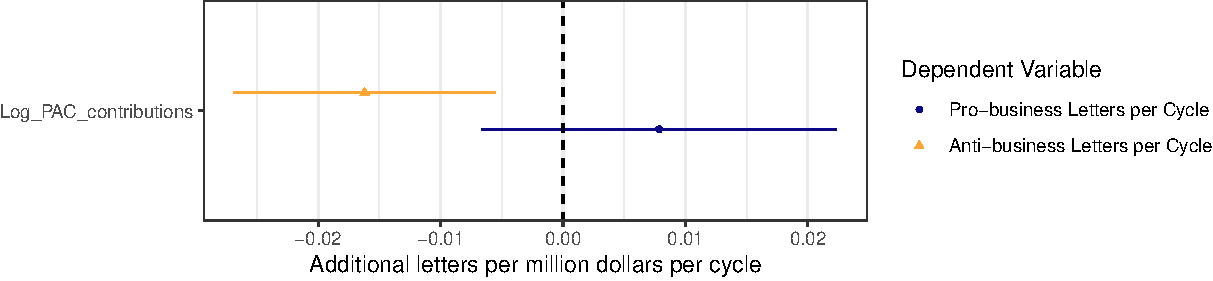
\includegraphics{Figs/models-2} \end{center}

\begin{Shaded}
\begin{Highlighting}[]
\NormalTok{knitr}\OperatorTok{::}\KeywordTok{kable}\NormalTok{(models }\OperatorTok{%>%}\StringTok{ }\NormalTok{dplyr}\OperatorTok{::}\KeywordTok{select}\NormalTok{(model, }\KeywordTok{everything}\NormalTok{()), }\DataTypeTok{digets =} \DecValTok{3}\NormalTok{, }\DataTypeTok{caption =} \StringTok{"Additional letters per million dollars per cycle"}\NormalTok{)}
\end{Highlighting}
\end{Shaded}

\begin{longtable}[]{@{}llrrrr@{}}
\caption{Additional letters per million dollars per
cycle}\tabularnewline
\toprule
model & term & estimate & std.error & statistic & p.value\tabularnewline
\midrule
\endfirsthead
\toprule
model & term & estimate & std.error & statistic & p.value\tabularnewline
\midrule
\endhead
Pro-business Letters per Cycle & (Intercept) & -1.5266248 & 0.0655695 &
-23.282533 & 0.0000000\tabularnewline
Pro-business Letters per Cycle & Log\_PAC\_contributions & 0.0078568 &
0.0074120 & 1.060010 & 0.2891400\tabularnewline
Anti-business Letters per Cycle & (Intercept) & -0.8402505 & 0.0468451 &
-17.936768 & 0.0000000\tabularnewline
Anti-business Letters per Cycle & Log\_PAC\_contributions & -0.0162125 &
0.0054405 & -2.979967 & 0.0028828\tabularnewline
\bottomrule
\end{longtable}

\begin{Shaded}
\begin{Highlighting}[]
\KeywordTok{write_lines}\NormalTok{(}
\NormalTok{  stargazer}\OperatorTok{::}\KeywordTok{stargazer}\NormalTok{(mProLog, mAntiLog),}
  \DataTypeTok{path =} \KeywordTok{here}\NormalTok{(}\StringTok{"FERC/tables/mProLog-mAntiLog.tex"}\NormalTok{))}
\end{Highlighting}
\end{Shaded}

\begin{verbatim}
## 
## % Table created by stargazer v.5.2.2 by Marek Hlavac, Harvard University. E-mail: hlavac at fas.harvard.edu
## % Date and time: Thu, May 09, 2019 - 10:00:10
## \begin{table}[!htbp] \centering 
##   \caption{} 
##   \label{} 
## \begin{tabular}{@{\extracolsep{5pt}}lcc} 
## \\[-1.8ex]\hline 
## \hline \\[-1.8ex] 
##  & \multicolumn{2}{c}{\textit{Dependent variable:}} \\ 
## \cline{2-3} 
## \\[-1.8ex] & ProBusiness\_Letters & AntiBusiness\_Letters \\ 
## \\[-1.8ex] & (1) & (2)\\ 
## \hline \\[-1.8ex] 
##  Log\_PAC\_contributions & 0.008 & $-$0.016$^{***}$ \\ 
##   & (0.007) & (0.005) \\ 
##   & & \\ 
##  Constant & $-$1.527$^{***}$ & $-$0.840$^{***}$ \\ 
##   & (0.066) & (0.047) \\ 
##   & & \\ 
## \hline \\[-1.8ex] 
## Observations & 5,170 & 5,170 \\ 
## Log Likelihood & $-$3,522.866 & $-$5,521.402 \\ 
## Akaike Inf. Crit. & 7,049.733 & 11,046.810 \\ 
## \hline 
## \hline \\[-1.8ex] 
## \textit{Note:}  & \multicolumn{2}{r}{$^{*}$p$<$0.1; $^{**}$p$<$0.05; $^{***}$p$<$0.01} \\ 
## \end{tabular} 
## \end{table}
\end{verbatim}

\begin{Shaded}
\begin{Highlighting}[]
\StringTok{"FERC/tables/mProLog-mAntiLog.tex"}
\end{Highlighting}
\end{Shaded}

\begin{verbatim}
## [1] "FERC/tables/mProLog-mAntiLog.tex"
\end{verbatim}

\begin{Shaded}
\begin{Highlighting}[]
\NormalTok{## PAC contributions over entire time period }
\NormalTok{models <-}\StringTok{ }\KeywordTok{tidy}\NormalTok{(mProTotal) }\OperatorTok{%>%}\StringTok{ }
\StringTok{  }\KeywordTok{mutate}\NormalTok{(}\DataTypeTok{model =} \StringTok{"Pro-business Letters per Cycle"}\NormalTok{) }\OperatorTok{%>%}\StringTok{ }
\StringTok{  }\KeywordTok{full_join}\NormalTok{(}\KeywordTok{tidy}\NormalTok{(mAntiTotal) }\OperatorTok{%>%}\StringTok{ }\KeywordTok{mutate}\NormalTok{(}\DataTypeTok{model =} \StringTok{"Anti-business Letters per Cycle"}\NormalTok{)) }

\KeywordTok{dplot}\NormalTok{(models) }\OperatorTok{+}\StringTok{ }
\StringTok{    }\KeywordTok{labs}\NormalTok{(}\DataTypeTok{x =} \StringTok{"Average additional letters per cycle per million dollars 1990-2014"}\NormalTok{)}
\end{Highlighting}
\end{Shaded}

\begin{center}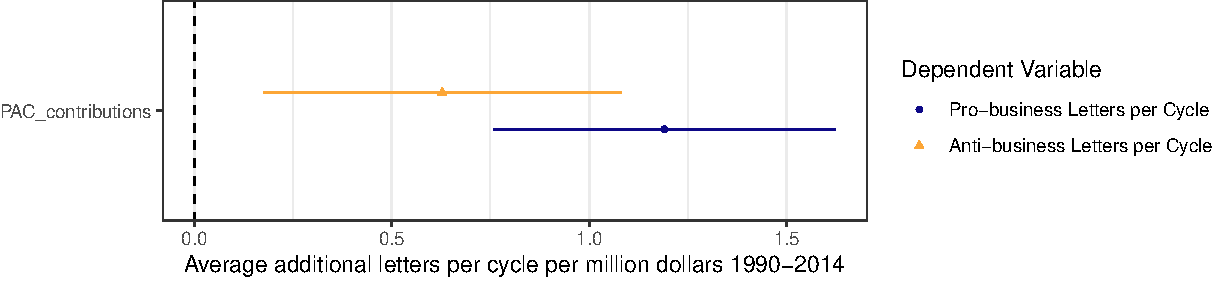
\includegraphics{Figs/models-3} \end{center}

\begin{Shaded}
\begin{Highlighting}[]
\NormalTok{knitr}\OperatorTok{::}\KeywordTok{kable}\NormalTok{(models}\OperatorTok{%>%}\StringTok{ }\NormalTok{dplyr}\OperatorTok{::}\KeywordTok{select}\NormalTok{(model, }\KeywordTok{everything}\NormalTok{()), }\DataTypeTok{digets =} \DecValTok{3}\NormalTok{, }\DataTypeTok{caption =} \StringTok{"Average additional letters per cycle per million dollars 1990-2014"}\NormalTok{)}
\end{Highlighting}
\end{Shaded}

\begin{longtable}[]{@{}llrrrr@{}}
\caption{Average additional letters per cycle per million dollars
1990-2014}\tabularnewline
\toprule
model & term & estimate & std.error & statistic & p.value\tabularnewline
\midrule
\endfirsthead
\toprule
model & term & estimate & std.error & statistic & p.value\tabularnewline
\midrule
\endhead
Pro-business Letters per Cycle & (Intercept) & -1.8666138 & 0.0941113 &
-19.834110 & 0.0000000\tabularnewline
Pro-business Letters per Cycle & PAC\_contributions & 1.1899212 &
0.2207469 & 5.390433 & 0.0000001\tabularnewline
Anti-business Letters per Cycle & (Intercept) & -1.2686438 & 0.0767932 &
-16.520266 & 0.0000000\tabularnewline
Anti-business Letters per Cycle & PAC\_contributions & 0.6281397 &
0.2310046 & 2.719166 & 0.0065447\tabularnewline
\bottomrule
\end{longtable}

\begin{Shaded}
\begin{Highlighting}[]
\KeywordTok{write_lines}\NormalTok{(}
\NormalTok{  stargazer}\OperatorTok{::}\KeywordTok{stargazer}\NormalTok{(mProTotal, mAntiTotal),}
  \DataTypeTok{path =} \KeywordTok{here}\NormalTok{(}\StringTok{"FERC/tables/mProTotal-mAntiTotal.tex"}\NormalTok{))}
\end{Highlighting}
\end{Shaded}

\begin{verbatim}
## 
## % Table created by stargazer v.5.2.2 by Marek Hlavac, Harvard University. E-mail: hlavac at fas.harvard.edu
## % Date and time: Thu, May 09, 2019 - 10:00:11
## \begin{table}[!htbp] \centering 
##   \caption{} 
##   \label{} 
## \begin{tabular}{@{\extracolsep{5pt}}lcc} 
## \\[-1.8ex]\hline 
## \hline \\[-1.8ex] 
##  & \multicolumn{2}{c}{\textit{Dependent variable:}} \\ 
## \cline{2-3} 
## \\[-1.8ex] & ProBusiness\_Letters\_Per\_Cycle & AntiBusiness\_Letters\_Per\_Cycle \\ 
## \\[-1.8ex] & (1) & (2)\\ 
## \hline \\[-1.8ex] 
##  PAC\_contributions & 1.190$^{***}$ & 0.628$^{***}$ \\ 
##   & (0.221) & (0.231) \\ 
##   & & \\ 
##  Constant & $-$1.867$^{***}$ & $-$1.269$^{***}$ \\ 
##   & (0.094) & (0.077) \\ 
##   & & \\ 
## \hline \\[-1.8ex] 
## Observations & 899 & 893 \\ 
## Log Likelihood & $-$Inf.000 & $-$Inf.000 \\ 
## Akaike Inf. Crit. & Inf.000 & Inf.000 \\ 
## \hline 
## \hline \\[-1.8ex] 
## \textit{Note:}  & \multicolumn{2}{r}{$^{*}$p$<$0.1; $^{**}$p$<$0.05; $^{***}$p$<$0.01} \\ 
## \end{tabular} 
## \end{table}
\end{verbatim}

\begin{Shaded}
\begin{Highlighting}[]
\StringTok{"FERC/tables/mProTotal-mAntiTotal.tex"}
\end{Highlighting}
\end{Shaded}

\begin{verbatim}
## [1] "FERC/tables/mProTotal-mAntiTotal.tex"
\end{verbatim}

\begin{Shaded}
\begin{Highlighting}[]
\NormalTok{## With party IV }
\NormalTok{models <-}\StringTok{ }\KeywordTok{tidy}\NormalTok{(mProParty) }\OperatorTok{%>%}\StringTok{ }
\StringTok{  }\KeywordTok{mutate}\NormalTok{(}\DataTypeTok{model =} \StringTok{"Pro-business Letters per Cycle"}\NormalTok{) }\OperatorTok{%>%}
\StringTok{  }\KeywordTok{full_join}\NormalTok{(}\KeywordTok{tidy}\NormalTok{(mAntiParty) }\OperatorTok{%>%}
\StringTok{              }\KeywordTok{mutate}\NormalTok{(}\DataTypeTok{model =} \StringTok{"Anti-business Letters per Cycle"}\NormalTok{)) }\OperatorTok{%>%}
\StringTok{  }\KeywordTok{mutate}\NormalTok{(}\DataTypeTok{term =} \KeywordTok{str_replace}\NormalTok{(term, }\StringTok{"party}\CharTok{\textbackslash{}\textbackslash{}}\StringTok{(R}\CharTok{\textbackslash{}\textbackslash{}}\StringTok{)"}\NormalTok{, }\StringTok{"Republican"}\NormalTok{))}

\KeywordTok{dplot}\NormalTok{(models) }\OperatorTok{+}\StringTok{ }
\StringTok{    }\KeywordTok{labs}\NormalTok{(}\DataTypeTok{x =} \StringTok{"Additional letters per cycle"}\NormalTok{)}
\end{Highlighting}
\end{Shaded}

\begin{center}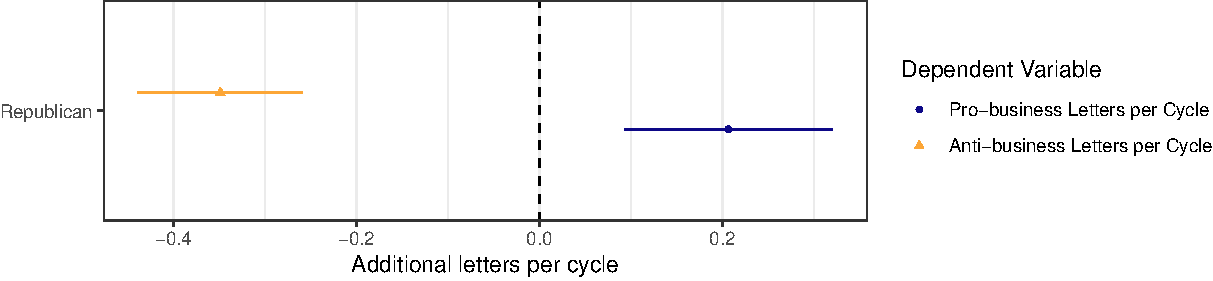
\includegraphics{Figs/models-4} \end{center}

\begin{Shaded}
\begin{Highlighting}[]
\NormalTok{knitr}\OperatorTok{::}\KeywordTok{kable}\NormalTok{(models}\OperatorTok{%>%}\StringTok{ }\NormalTok{dplyr}\OperatorTok{::}\KeywordTok{select}\NormalTok{(model, }\KeywordTok{everything}\NormalTok{()), }\DataTypeTok{digets =} \DecValTok{3}\NormalTok{, }\DataTypeTok{caption =} \StringTok{"Average additional letters per cycle"}\NormalTok{)}
\end{Highlighting}
\end{Shaded}

\begin{longtable}[]{@{}llrrrr@{}}
\caption{Average additional letters per cycle}\tabularnewline
\toprule
model & term & estimate & std.error & statistic & p.value\tabularnewline
\midrule
\endfirsthead
\toprule
model & term & estimate & std.error & statistic & p.value\tabularnewline
\midrule
\endhead
Pro-business Letters per Cycle & (Intercept) & -1.2389768 & 0.0425242 &
-29.135818 & 0.0000000\tabularnewline
Pro-business Letters per Cycle & Republican & 0.2063579 & 0.0580165 &
3.556881 & 0.0003753\tabularnewline
Anti-business Letters per Cycle & (Intercept) & -0.4793716 & 0.0290854 &
-16.481534 & 0.0000000\tabularnewline
Anti-business Letters per Cycle & Republican & -0.3483375 & 0.0459881 &
-7.574522 & 0.0000000\tabularnewline
\bottomrule
\end{longtable}

\begin{Shaded}
\begin{Highlighting}[]
\KeywordTok{write_lines}\NormalTok{(}
\NormalTok{  stargazer}\OperatorTok{::}\KeywordTok{stargazer}\NormalTok{(mProParty, mAntiParty),}
  \DataTypeTok{path =} \KeywordTok{here}\NormalTok{(}\StringTok{"FERC/tables/mProParty-mAntiParty.tex"}\NormalTok{))}
\end{Highlighting}
\end{Shaded}

\begin{verbatim}
## 
## % Table created by stargazer v.5.2.2 by Marek Hlavac, Harvard University. E-mail: hlavac at fas.harvard.edu
## % Date and time: Thu, May 09, 2019 - 10:00:11
## \begin{table}[!htbp] \centering 
##   \caption{} 
##   \label{} 
## \begin{tabular}{@{\extracolsep{5pt}}lcc} 
## \\[-1.8ex]\hline 
## \hline \\[-1.8ex] 
##  & \multicolumn{2}{c}{\textit{Dependent variable:}} \\ 
## \cline{2-3} 
## \\[-1.8ex] & ProBusiness\_Letters & AntiBusiness\_Letters \\ 
## \\[-1.8ex] & (1) & (2)\\ 
## \hline \\[-1.8ex] 
##  party(R) & 0.206$^{***}$ & $-$0.348$^{***}$ \\ 
##   & (0.058) & (0.046) \\ 
##   & & \\ 
##  Constant & $-$1.239$^{***}$ & $-$0.479$^{***}$ \\ 
##   & (0.043) & (0.029) \\ 
##   & & \\ 
## \hline \\[-1.8ex] 
## Observations & 3,712 & 3,712 \\ 
## Log Likelihood & $-$3,121.183 & $-$4,843.850 \\ 
## Akaike Inf. Crit. & 6,246.367 & 9,691.701 \\ 
## \hline 
## \hline \\[-1.8ex] 
## \textit{Note:}  & \multicolumn{2}{r}{$^{*}$p$<$0.1; $^{**}$p$<$0.05; $^{***}$p$<$0.01} \\ 
## \end{tabular} 
## \end{table}
\end{verbatim}

\begin{Shaded}
\begin{Highlighting}[]
\StringTok{"FERC/tables/mProParty-mAntiParty.tex"}
\end{Highlighting}
\end{Shaded}

\begin{verbatim}
## [1] "FERC/tables/mProParty-mAntiParty.tex"
\end{verbatim}

\begin{Shaded}
\begin{Highlighting}[]
\KeywordTok{write_lines}\NormalTok{(}
\NormalTok{  stargazer}\OperatorTok{::}\KeywordTok{stargazer}\NormalTok{(mAll, mPro, mAnti,mNonConstituent, mProLog, mAntiLog, mProParty, mProTotal, mAntiTotal, mAntiParty),}
  \DataTypeTok{path =} \KeywordTok{here}\NormalTok{(}\StringTok{"FERC/tables/m.tex"}\NormalTok{))}
\end{Highlighting}
\end{Shaded}

\begin{verbatim}
## 
## % Table created by stargazer v.5.2.2 by Marek Hlavac, Harvard University. E-mail: hlavac at fas.harvard.edu
## % Date and time: Thu, May 09, 2019 - 10:00:11
## \begin{table}[!htbp] \centering 
##   \caption{} 
##   \label{} 
## \begin{tabular}{@{\extracolsep{5pt}}lcccccccccc} 
## \\[-1.8ex]\hline 
## \hline \\[-1.8ex] 
##  & \multicolumn{10}{c}{\textit{Dependent variable:}} \\ 
## \cline{2-11} 
## \\[-1.8ex] & All\_Letters & ProBusiness\_Letters & AntiBusiness\_Letters & Non\_Constituent\_Letters & ProBusiness\_Letters & AntiBusiness\_Letters & ProBusiness\_Letters & ProBusiness\_Letters\_Per\_Cycle & AntiBusiness\_Letters\_Per\_Cycle & AntiBusiness\_Letters \\ 
## \\[-1.8ex] & (1) & (2) & (3) & (4) & (5) & (6) & (7) & (8) & (9) & (10)\\ 
## \hline \\[-1.8ex] 
##  PAC\_contributions & 3.106$^{***}$ & 2.242$^{***}$ & 0.476 & 0.00000$^{***}$ &  &  &  & 1.190$^{***}$ & 0.628$^{***}$ &  \\ 
##   & (0.267) & (0.600) & (0.546) & (0.00000) &  &  &  & (0.221) & (0.231) &  \\ 
##   & & & & & & & & & & \\ 
##  Log\_PAC\_contributions &  &  &  &  & 0.008 & $-$0.016$^{***}$ &  &  &  &  \\ 
##   &  &  &  &  & (0.007) & (0.005) &  &  &  &  \\ 
##   & & & & & & & & & & \\ 
##  party(R) &  &  &  &  &  &  & 0.206$^{***}$ &  &  & $-$0.348$^{***}$ \\ 
##   &  &  &  &  &  &  & (0.058) &  &  & (0.046) \\ 
##   & & & & & & & & & & \\ 
##  Constant & $-$0.107$^{***}$ & $-$1.527$^{***}$ & $-$0.977$^{***}$ & $-$0.107$^{***}$ & $-$1.527$^{***}$ & $-$0.840$^{***}$ & $-$1.239$^{***}$ & $-$1.867$^{***}$ & $-$1.269$^{***}$ & $-$0.479$^{***}$ \\ 
##   & (0.016) & (0.034) & (0.027) & (0.016) & (0.066) & (0.047) & (0.043) & (0.094) & (0.077) & (0.029) \\ 
##   & & & & & & & & & & \\ 
## \hline \\[-1.8ex] 
## Observations & 5,170 & 5,170 & 5,170 & 5,170 & 5,170 & 5,170 & 3,712 & 899 & 893 & 3,712 \\ 
## Log Likelihood & $-$10,579.530 & $-$3,517.320 & $-$5,525.361 & $-$10,579.530 & $-$3,522.866 & $-$5,521.402 & $-$3,121.183 & $-$Inf.000 & $-$Inf.000 & $-$4,843.850 \\ 
## Akaike Inf. Crit. & 21,163.050 & 7,038.639 & 11,054.720 & 21,163.050 & 7,049.733 & 11,046.810 & 6,246.367 & Inf.000 & Inf.000 & 9,691.701 \\ 
## \hline 
## \hline \\[-1.8ex] 
## \textit{Note:}  & \multicolumn{10}{r}{$^{*}$p$<$0.1; $^{**}$p$<$0.05; $^{***}$p$<$0.01} \\ 
## \end{tabular} 
## \end{table}
\end{verbatim}

\subsection{PAC-level}\label{pac-level}

\subsubsection{Before matching projects and companies to their parent
companies:}\label{before-matching-projects-and-companies-to-their-parent-companies}

\begin{Shaded}
\begin{Highlighting}[]
\CommentTok{# letter count per pac ~ pac contributions (lots of 0$-0letter pairs )}
\CommentTok{# 1. id pacs per letter - spit letters matching several pacs }
\CommentTok{# 2. count up per member }
\CommentTok{# 3. add 0s for all other pac-member-cycle compinations }
\CommentTok{# merge in with contributions per pac per member }

\CommentTok{# First, clean up the contributions data a bit}

\CommentTok{# a helper function to concat unique strings}
\NormalTok{unique_string <-}\StringTok{ }\NormalTok{. }\OperatorTok{%>%}\StringTok{ }
\StringTok{  }\KeywordTok{str_split}\NormalTok{(}\StringTok{";"}\NormalTok{) }\OperatorTok{%>%}\StringTok{ }
\StringTok{  }\CommentTok{# select unique ones}
\StringTok{  }\KeywordTok{unlist}\NormalTok{() }\OperatorTok{%>%}\StringTok{ }
\StringTok{  }\KeywordTok{unique}\NormalTok{() }\OperatorTok{%>%}\StringTok{ }
\StringTok{  }\KeywordTok{trimws}\NormalTok{() }\OperatorTok{%>%}\StringTok{ }
\StringTok{  }\CommentTok{# paste them back together to retrun a single value }
\StringTok{  }\KeywordTok{paste}\NormalTok{(}\DataTypeTok{collapse =} \StringTok{";"}\NormalTok{) }\OperatorTok{%>%}
\StringTok{  }\KeywordTok{str_remove_all}\NormalTok{(}\StringTok{"na;|;na$|NA;|;NA$"}\NormalTok{)}

\CommentTok{# Just the PAC names and IDs from the contributions matrix (will merge in relevent contributions later)}
\NormalTok{PACs <-}\StringTok{ }\NormalTok{contrib_matrix }\OperatorTok{%>%}\StringTok{ }
\StringTok{  }\KeywordTok{select}\NormalTok{(comid, UltOrg,Affiliate,PACShort) }\OperatorTok{%>%}\StringTok{ }\KeywordTok{distinct}\NormalTok{() }\OperatorTok{%>%}\StringTok{ }
\StringTok{  }\CommentTok{# make a full list of pac-affiliated orgs}
\StringTok{  }\KeywordTok{group_by}\NormalTok{(comid) }\OperatorTok{%>%}
\StringTok{  }\KeywordTok{mutate}\NormalTok{(}\DataTypeTok{UltOrg2 =} \KeywordTok{str_c}\NormalTok{(UltOrg,Affiliate,PACShort, }\DataTypeTok{sep =} \StringTok{";"}\NormalTok{) }\OperatorTok{%>%}\StringTok{ }
\StringTok{           }\KeywordTok{tolower}\NormalTok{() }\OperatorTok{%>%}\StringTok{ }
\StringTok{           }\CommentTok{# select unique ones}
\StringTok{           }\KeywordTok{unique_string}\NormalTok{())}

\CommentTok{# A function to get matching names}
\NormalTok{get_pac <-}\StringTok{ }\ControlFlowTok{function}\NormalTok{(corp, PAC)\{}
  \KeywordTok{ifelse}\NormalTok{(}\KeywordTok{str_detect}\NormalTok{(}\KeywordTok{tolower}\NormalTok{(PAC), }\KeywordTok{tolower}\NormalTok{(corp)), PAC, }\OtherTok{NA}\NormalTok{)}
\NormalTok{\}}

\CommentTok{# A function to get IDs where names match }
\NormalTok{get_pacID <-}\StringTok{ }\ControlFlowTok{function}\NormalTok{(corp, PAC, PACid)\{}
  \KeywordTok{ifelse}\NormalTok{(}\KeywordTok{str_detect}\NormalTok{(}\KeywordTok{tolower}\NormalTok{(PAC), }\KeywordTok{tolower}\NormalTok{(corp)), PACid, }\OtherTok{NA}\NormalTok{) }
\NormalTok{\}}


\CommentTok{# corp = "Exxon"}

\CommentTok{# A function to augment the PAC data with any matching company names }
\NormalTok{get_pacs <-}\StringTok{ }\ControlFlowTok{function}\NormalTok{(corp)\{}
\NormalTok{PACs }\OperatorTok{%>%}\StringTok{ }
\StringTok{    }\KeywordTok{mutate}\NormalTok{(}\DataTypeTok{pacs =} \KeywordTok{get_pac}\NormalTok{(}\KeywordTok{tolower}\NormalTok{(corp), UltOrg2),}
           \DataTypeTok{pacIDs =} \KeywordTok{get_pacID}\NormalTok{(}\KeywordTok{tolower}\NormalTok{(corp), UltOrg2, comid)) }\OperatorTok{%>%}\StringTok{ }
\StringTok{    }\KeywordTok{ungroup}\NormalTok{() }\OperatorTok{%>%}\StringTok{ }
\StringTok{    }\KeywordTok{select}\NormalTok{(pacs, pacIDs) }\OperatorTok{%>%}\StringTok{ }
\StringTok{    }\KeywordTok{distinct}\NormalTok{() }\OperatorTok{%>%}\StringTok{ }
\StringTok{    }\KeywordTok{summarise_all}\NormalTok{(unique_string) }\OperatorTok{%>%}\StringTok{ }
\StringTok{    }\KeywordTok{mutate}\NormalTok{(}\DataTypeTok{company_short =}\NormalTok{ corp)}
\NormalTok{\}}

\CommentTok{# }\AlertTok{TESTING}\CommentTok{ }
\CommentTok{# corp = "Exxon"}
\CommentTok{# get_pacs(corp)}
\CommentTok{# corp <- dcorps$company_short[1]}
\CommentTok{# get_pacs(corp)}

\NormalTok{crosswalk <-}\StringTok{ }\KeywordTok{map_dfr}\NormalTok{(dcorps}\OperatorTok{$}\NormalTok{company_short, get_pacs)}

\NormalTok{crosswalk }\OperatorTok{%<>%}\StringTok{ }\KeywordTok{distinct}\NormalTok{()}

\CommentTok{# use crosswalk to merge in contribution data }
\NormalTok{dpacs <-}\StringTok{ }\NormalTok{dcorps }\OperatorTok{%>%}\StringTok{ }
\StringTok{  }\KeywordTok{full_join}\NormalTok{(crosswalk) }\OperatorTok{%>%}\StringTok{ }
\StringTok{  }\CommentTok{# letters per year per pac}
\StringTok{  }\KeywordTok{select}\NormalTok{(ID, position, company_short, position, pacs, pacIDs) }\OperatorTok{%>%}\StringTok{ }
\StringTok{  }\KeywordTok{distinct}\NormalTok{() }\OperatorTok{%>%}\StringTok{ }
\StringTok{  }\KeywordTok{mutate}\NormalTok{(}\DataTypeTok{pacIDs =} \KeywordTok{str_split}\NormalTok{(pacIDs, }\StringTok{";"}\NormalTok{)) }\OperatorTok{%>%}\StringTok{ }
\StringTok{  }\KeywordTok{unnest}\NormalTok{(pacIDs) }\OperatorTok{%>%}\StringTok{ }
\StringTok{  }\KeywordTok{distinct}\NormalTok{() }\OperatorTok{%>%}\StringTok{ }
\StringTok{  }\CommentTok{# merge in pac totals}
\StringTok{  }\KeywordTok{rename}\NormalTok{(}\DataTypeTok{comid =}\NormalTok{ pacIDs) }\OperatorTok{%>%}\StringTok{ }
\StringTok{  }\CommentTok{# merge in contribution data}
\StringTok{  }\KeywordTok{left_join}\NormalTok{(contrib_matrix) }\CommentTok{# %>% group_by(comid, position) %>% summarise(PAC_contributions)}

\NormalTok{dpacs }\OperatorTok{%<>%}\StringTok{ }
\StringTok{  }\KeywordTok{ungroup}\NormalTok{() }\OperatorTok{%>%}\StringTok{ }
\StringTok{  }\KeywordTok{filter}\NormalTok{(}\OperatorTok{!}\KeywordTok{is.na}\NormalTok{(ID), }\OperatorTok{!}\KeywordTok{is.na}\NormalTok{(comid)) }\OperatorTok{%>%}\StringTok{ }
\StringTok{  }\KeywordTok{select}\NormalTok{(ID, icpsryear, cycle, name_state, position, company_short, pacs, comid, PAC_contributions) }\OperatorTok{%>%}\StringTok{ }
\StringTok{  }\KeywordTok{distinct}\NormalTok{()}
\end{Highlighting}
\end{Shaded}

\paragraph{Pro-business letters linked to PAC
contributions:}\label{pro-business-letters-linked-to-pac-contributions}

\begin{Shaded}
\begin{Highlighting}[]
\NormalTok{dpacs }\OperatorTok{%>%}\StringTok{ }
\StringTok{  }\KeywordTok{filter}\NormalTok{(position }\OperatorTok{%in%}\StringTok{ }\KeywordTok{c}\NormalTok{(}\StringTok{"ProBusiness"}\NormalTok{, }\StringTok{"ProProject"}\NormalTok{)) }\OperatorTok{%>%}\StringTok{ }
\StringTok{  }\CommentTok{# select letters with an identified person}
\StringTok{  }\KeywordTok{drop_na}\NormalTok{(name_state, ID) }\OperatorTok{%>%}
\StringTok{  }\KeywordTok{group_by}\NormalTok{(name_state, cycle, position, company_short, pacs, comid) }\OperatorTok{%>%}\StringTok{ }
\StringTok{  }\KeywordTok{distinct}\NormalTok{()}\OperatorTok{%>%}\StringTok{  }\KeywordTok{summarise}\NormalTok{(}\DataTypeTok{PAC_contributions =} \KeywordTok{sum}\NormalTok{(PAC_contributions, }\DataTypeTok{na.rm =}\NormalTok{ T),}
                           \CommentTok{# }\AlertTok{FIXME}\CommentTok{ }
                           \CommentTok{# SHOULD NOT NEED UNIQUE HERE }
            \DataTypeTok{Letter_IDs =} \KeywordTok{paste}\NormalTok{(}\KeywordTok{unique}\NormalTok{(ID), }\DataTypeTok{collapse =} \StringTok{";"}\NormalTok{)) }\OperatorTok{%>%}\StringTok{ }
\StringTok{  }\KeywordTok{ungroup}\NormalTok{() }\OperatorTok{%>%}\StringTok{ }
\StringTok{  }\KeywordTok{group_by}\NormalTok{(position)  }\OperatorTok{%>%}
\StringTok{  }\KeywordTok{top_n}\NormalTok{(}\DecValTok{10}\NormalTok{, PAC_contributions) }\OperatorTok{%>%}\StringTok{ }
\StringTok{  }\NormalTok{knitr}\OperatorTok{::}\KeywordTok{kable}\NormalTok{()}
\end{Highlighting}
\end{Shaded}

\paragraph{Anti-business letters linked to PAC
contributions:}\label{anti-business-letters-linked-to-pac-contributions}

\begin{Shaded}
\begin{Highlighting}[]
\NormalTok{dpacs }\OperatorTok{%>%}\StringTok{ }
\StringTok{  }\KeywordTok{filter}\NormalTok{(position }\OperatorTok{%in%}\StringTok{ }\KeywordTok{c}\NormalTok{(}\StringTok{"AntiBusiness"}\NormalTok{, }\StringTok{"AntiProject"}\NormalTok{)) }\OperatorTok{%>%}\StringTok{ }
\StringTok{  }\KeywordTok{left_join}\NormalTok{(d }\OperatorTok{%>%}\StringTok{ }\KeywordTok{select}\NormalTok{(ID, Constituent) }\OperatorTok{%>%}\StringTok{ }\KeywordTok{distinct}\NormalTok{() ) }\OperatorTok{%>%}\StringTok{ }
\StringTok{  }\KeywordTok{filter}\NormalTok{(Constituent }\OperatorTok{==}\StringTok{ "No"}\NormalTok{) }\OperatorTok{%>%}
\StringTok{  }\CommentTok{# select letters with an identified person}
\StringTok{  }\KeywordTok{drop_na}\NormalTok{(name_state, ID) }\OperatorTok{%>%}
\StringTok{  }\KeywordTok{group_by}\NormalTok{(name_state, cycle, position, company_short, pacs, comid) }\OperatorTok{%>%}\StringTok{ }
\StringTok{  }\KeywordTok{distinct}\NormalTok{()}\OperatorTok{%>%}\StringTok{  }\KeywordTok{summarise}\NormalTok{(}\DataTypeTok{PAC_contributions =} \KeywordTok{sum}\NormalTok{(PAC_contributions, }\DataTypeTok{na.rm =}\NormalTok{ T),}
                           \CommentTok{# }\AlertTok{FIXME}\CommentTok{ }
                           \CommentTok{# SHOULD NOT NEED UNIQUE HERE }
            \DataTypeTok{Letter_IDs =} \KeywordTok{paste}\NormalTok{(}\KeywordTok{unique}\NormalTok{(ID), }\DataTypeTok{collapse =} \StringTok{";"}\NormalTok{)) }\OperatorTok{%>%}\StringTok{ }
\StringTok{  }\KeywordTok{ungroup}\NormalTok{() }\OperatorTok{%>%}\StringTok{ }
\StringTok{  }\KeywordTok{group_by}\NormalTok{(position)  }\OperatorTok{%>%}
\StringTok{  }\KeywordTok{top_n}\NormalTok{(}\DecValTok{10}\NormalTok{, PAC_contributions) }\OperatorTok{%>%}\StringTok{ }
\StringTok{  }\NormalTok{knitr}\OperatorTok{::}\KeywordTok{kable}\NormalTok{()}

\CommentTok{#Before connecting companies to the PAC donations of their parent companies, we find `r sum(!is.na(dpacs$ID))` letters with a pack donation.}
\end{Highlighting}
\end{Shaded}

\begin{verbatim}
################################################   
# merge in and split out parent corps 

# TABLE 
letterID 
date
member
district 
committee 
position 
company
pac 
ammount 


# risiduals 
\end{verbatim}

\section{About FERC}\label{about-ferc}

FERC regulates electricity markets, oil and gas pipelines, and
hydropower and gas export terminal projects.

FERC controls pipeline market entry.

\subsection{Letters on behalf of projects in their
districts}\label{letters-on-behalf-of-projects-in-their-districts}

TODO

\subsection{Letters are on behalf of
donors}\label{letters-are-on-behalf-of-donors}

TODO

\subsection{Comparing FERC to other
agencies}\label{comparing-ferc-to-other-agencies}

TODO

\section{TO DO}\label{to-do}

\begin{itemize}
\tightlist
\item
  Fix Goode, who is being double counted as an R and I
\item
  add company names from company scraper to google sheet
\item
  template to match company names to donation (lobbyview, DIME)
\item
  template match company names to industry codes (center for responsive
  politics)
\end{itemize}

\subsection{SHORT TERM}\label{short-term}

\begin{itemize}
\tightlist
\item
  letters per company
\item
  letters per company pac (before and after merging in partent
  companies)
\end{itemize}

\subsection{LONG TERM}\label{long-term}

\subsection{DONE}\label{done}

\begin{itemize}
\tightlist
\item
  add clean text from scraper to google sheet
\item
  fix clean function to pull and combine new data
\item
  link industry codes to CRP PAC committee classification
\end{itemize}

\begin{enumerate}
\def\labelenumi{\arabic{enumi}.}
\tightlist
\item
  Identify relevent industry codes
\item
  Get cycle-specific PAC classification for those industry codes
\item
  Subset dime to those PAC classification
\end{enumerate}

\section{References}\label{references}


\end{document}
